\documentclass[aspectratio=169]{beamer}
% ============================================================================
% HEC Montréal MBA -- ECON50803: Macroeconomic Environment
% Shared Beamer Preamble
% ============================================================================

% --- Theme and base settings ------------------------------------------------
\usetheme{default}
\setbeamersize{text margin left=1.2cm, text margin right=1.2cm}

% --- Fonts ------------------------------------------------------------------
% Sans-serif throughout for a business look (comment out FiraSans if unavailable)
\usepackage[sfdefault,light]{FiraSans}
\usepackage{FiraMono}
\usepackage[T1]{fontenc}
\usepackage[utf8]{inputenc}
\setbeamerfont{title}{series=\bfseries, size=\Large}
\setbeamerfont{frametitle}{series=\bfseries, size=\large}
\setbeamerfont{framesubtitle}{series=\mdseries, size=\normalsize}

% --- Colors -----------------------------------------------------------------
\definecolor{HECnavy}{HTML}{002855}
\definecolor{HECgreen}{HTML}{26d07c}
\definecolor{HECcoral}{HTML}{ff585d}
\definecolor{HECtext}{HTML}{2D3748}
\definecolor{HECgray}{HTML}{94A3B8}
\definecolor{HEClightgray}{HTML}{F1F5F9}
\definecolor{HEClightblue}{HTML}{E8EDF3}

% Beamer color assignments
\setbeamercolor{normal text}{fg=HECtext}
\setbeamercolor{title}{fg=HECnavy}
\setbeamercolor{frametitle}{fg=HECnavy}
\setbeamercolor{structure}{fg=HECnavy}
\setbeamercolor{background canvas}{bg=white}
\setbeamercolor{alerted text}{fg=HECcoral}
\setbeamercolor{example text}{fg=HECgreen}
\hypersetup{colorlinks, linkcolor=HECnavy, urlcolor=HECnavy, citecolor=HECtext}

% --- Navigation and chrome --------------------------------------------------
\setbeamertemplate{navigation symbols}{}

% Frame title: bold text with a thin accent line
\setbeamertemplate{frametitle}{%
   \vspace{0.25cm}%
   {\usebeamerfont{frametitle}\usebeamercolor[fg]{frametitle}\insertframetitle}%
   \ifx\insertframesubtitle\empty\else%
      \\[2pt]{\usebeamerfont{framesubtitle}\textcolor{HECgray}{\insertframesubtitle}}%
   \fi%
   \\[-4pt]\textcolor{HECgreen}{\rule{2.5cm}{1.5pt}}%
   \\[-2pt]%
}

% Footer: course name left, slide number right, thin rule above
\setbeamertemplate{footline}{%
   \vspace{-0.1cm}%
   \hbox to \paperwidth{%
      \hspace{1.2cm}%
      \textcolor{HEClightgray}{\rule{0.84\paperwidth}{0.4pt}}%
      \hspace{1.2cm}%
   }%
   \vspace{0.05cm}%
   \hbox to \paperwidth{%
      \hspace{1.2cm}%
      {\scriptsize\textcolor{HECgray}{ECON 50803\enspace\textbar\enspace Environnement macroéconomique}}%
      \hfill%
      {\scriptsize\textcolor{HECgray}{\insertframenumber}}%
      \hspace{1.2cm}%
   }%
   \vspace{0.15cm}%
}

% --- Itemize/enumerate styling ----------------------------------------------
\setbeamertemplate{itemize item}{\textcolor{HECnavy}{$\bullet$}}
\setbeamertemplate{itemize subitem}{\textcolor{HECgray}{$\bullet$}}
\setbeamertemplate{itemize subsubitem}{\textcolor{HECgray}{\scalebox{0.6}{$\blacktriangleright$}}}
\setbeamertemplate{enumerate item}{\textcolor{HECnavy}{\bfseries\insertenumlabel.}}
\setbeamertemplate{enumerate subitem}{\textcolor{HECgray}{\insertsubenumlabel.}}

% --- Packages ---------------------------------------------------------------
\usepackage{
   tikz, caption, subcaption, ragged2e, amsmath, bm,
   makecell, threeparttable, booktabs, mathtools,
   multirow, calc, hyperref, tabularx, colortbl,
   transparent, tcolorbox, xcolor, graphicx
}
\usepackage[round]{natbib}
\usetikzlibrary{decorations.pathreplacing, decorations.markings, calc, arrows.meta, positioning}
\usepackage[absolute,overlay]{textpos}
\captionsetup[figure]{labelformat=empty, font=small, textfont=it}
\captionsetup[table]{labelformat=empty, font=small}
\setlength{\belowcaptionskip}{0cm}
\apptocmd{\frame}{}{\justifying}

% --- Paths ------------------------------------------------------------------
\graphicspath{{../Figures/}}
\newcommand*\includetables[1]{\input{../Tables/#1.tex}}

% --- Mathematical commands --------------------------------------------------
\DeclareMathOperator*{\argmax}{arg\,max}
\newcommand{\partialof}[2]{\frac{\partial #1}{\partial #2}}
\newcommand{\totalof}[2]{\frac{\text{d}#1}{\text{d}#2}}
\newcommand{\pctchg}[1]{\%\Delta #1}
\newcommand{\smallquad}{\hspace{0.5em}}

% --- Resize equation command ------------------------------------------------
\newcommand{\resizeeq}[2]{\resizebox{#2\hsize}{!}{$#1$}}

% ============================================================================
% CUSTOM SLIDE TYPES
% ============================================================================

% --- Title slide (call with \titleframe) ------------------------------------
\newcommand{\titleframe}{%
   {\setbeamertemplate{footline}{}%
   \begin{frame}[plain]
      \begin{tikzpicture}[remember picture, overlay]
         % Navy accent bar on the left
         \fill[HECnavy] (current page.north west) rectangle
            ([xshift=0.6cm]current page.south west);
         % Green accent line
         \fill[HECgreen] ([xshift=0.6cm]current page.north west) rectangle
            ([xshift=0.65cm]current page.south west);
      \end{tikzpicture}
      \vspace{1cm}
      \hspace{0.6cm}%
      \begin{minipage}{0.85\textwidth}
         {\usebeamerfont{title}\usebeamercolor[fg]{title}\inserttitle}
         \\[12pt]
         \textcolor{HECgreen}{\rule{3cm}{2pt}}
         \\[12pt]
         {\large\textcolor{HECgray}{\insertauthor}}
         \\[6pt]
         {\normalsize\textcolor{HECgray}{\insertdate}}
      \end{minipage}
      \vfill
      \hspace{0.6cm}%
      {\footnotesize\textcolor{HECgray}{HEC Montréal \enspace\textbar\enspace MBA}}
      \vspace{0.5cm}
   \end{frame}}%
}

% --- Section divider slide --------------------------------------------------
\newcommand{\sectionframe}[1]{%
   {\setbeamertemplate{footline}{}%
   \begin{frame}[plain]
      \begin{tikzpicture}[remember picture, overlay]
         \fill[HECnavy] ([shift={(-1pt,1pt)}]current page.north west) rectangle
            ([shift={(1pt,-1pt)}]current page.south east);
         \node[anchor=center] at (current page.center) {%
            \begin{minipage}{0.8\paperwidth}
               \centering
               {\LARGE\bfseries\textcolor{white}{#1}}
               \\[12pt]
               \textcolor{HECgreen}{\rule{3cm}{2pt}}
            \end{minipage}
         };
      \end{tikzpicture}
   \end{frame}}%
}

% ============================================================================
% CUSTOM BOX ENVIRONMENTS
% ============================================================================

% Key Insight (green accent)
\newtcolorbox{keyinsight}[1][Point clé]{%
   colback=HECgreen!5,
   colframe=HECgreen,
   boxrule=0pt,
   leftrule=3pt,
   arc=8pt,
   title={\textcolor{HECgreen}{\bfseries #1}},
   coltitle=HECgreen,
   fonttitle=\bfseries,
   attach title to upper={\\[4pt]},
   left=10pt, right=10pt, top=6pt, bottom=6pt
}

% Business Implication (navy accent)
\newtcolorbox{bizimplication}[1][Implication d'affaires]{%
   colback=HECnavy!5,
   colframe=HECnavy,
   boxrule=0pt,
   leftrule=3pt,
   arc=8pt,
   title={\textcolor{HECnavy}{\bfseries #1}},
   coltitle=HECnavy,
   fonttitle=\bfseries,
   attach title to upper={\\[4pt]},
   left=10pt, right=10pt, top=6pt, bottom=6pt
}

% Warning / Important (coral accent)
\newtcolorbox{warning}[1][Important]{%
   colback=HECcoral!5,
   colframe=HECcoral,
   boxrule=0pt,
   leftrule=3pt,
   arc=8pt,
   title={\textcolor{HECcoral}{\bfseries #1}},
   coltitle=HECcoral,
   fonttitle=\bfseries,
   attach title to upper={\\[4pt]},
   left=10pt, right=10pt, top=6pt, bottom=6pt
}

% Definition (gray background)
\newtcolorbox{defbox}[1][Définition]{%
   colback=HEClightgray,
   colframe=HEClightgray,
   boxrule=0pt,
   leftrule=3pt,
   arc=8pt,
   left=10pt, right=10pt, top=6pt, bottom=6pt,
   title={\textcolor{HECnavy}{\bfseries #1}},
   coltitle=HECnavy,
   fonttitle=\bfseries,
   attach title to upper={\\[4pt]}
}

% In-Class Exercise (coral accent)
\newtcolorbox{exercise}[1][Exercice]{%
   colback=HECcoral!5,
   colframe=HECcoral,
   boxrule=0pt,
   leftrule=3pt,
   arc=8pt,
   title={\textcolor{HECcoral}{\bfseries #1}},
   coltitle=HECcoral,
   fonttitle=\bfseries,
   attach title to upper={\\[4pt]},
   left=10pt, right=10pt, top=6pt, bottom=6pt
}

% ============================================================================
% NEWSPAPER HEADLINES SLIDE TEMPLATE
% ============================================================================
% Usage: inside a frame, open a tikzpicture[remember picture, overlay], then:
%   \setcounter{newshl}{0}
%   \newsheadline{Newspaper Name}{``Headline text''}   % up to 6 entries
%   \headlinesoverlay{Large overlay text}               % optional 2nd slide
%
% Headlines are auto-positioned in a 2×3 staggered grid (left/right alternating).
%
% Logo support: place PNG files in Figures/logos/ (e.g., ft.png, economist.png).
% Use the optional argument to specify the logo file (without extension):
%   \newsheadline[ft]{Financial Times}{Headline text}   % logo + bold headline
%   \newsheadline{The Economist}{``Headline text''}      % text-only fallback

\newcounter{newshl}

\newcommand{\newsheadline}[3][]{%
   % #1 = optional logo file key (e.g., ft → logos/ft.png)
   % #2 = newspaper name (text fallback when no logo)
   % #3 = headline text
   \stepcounter{newshl}%
   \pgfmathsetmacro{\hlrow}{int((\thenewshl-1)/2)}%
   \pgfmathsetmacro{\hlcol}{int(mod(\thenewshl-1,2))}%
   \pgfmathsetmacro{\hlx}{0.8 + \hlcol * 7.8}%
   \pgfmathsetmacro{\hly}{-1.5 - \hlrow * 2.0}%
   \node[anchor=north west]
      at ([shift={(\hlx cm,\hly cm)}]current page.north west) {%
      \ifx\\#1\\%
         \begin{minipage}[t]{5.8cm}%
            \textbf{\textcolor{HECgray}{\footnotesize\MakeUppercase{#2}}}%
            \\[-1pt]%
            {\small\itshape #3}%
         \end{minipage}%
      \else%
         \begin{minipage}[c]{1.2cm}%
            \includegraphics[height=1.2cm]{logos/#1}%
         \end{minipage}%
         \hspace{6pt}%
         \begin{minipage}[c][1.2cm][c]{4.3cm}%
            \raggedright{\small\textcolor{HECtext!75}{#3}}%
         \end{minipage}%
      \fi%
   };%
}

\newcommand{\headlinesoverlay}[1]{%
   \only<2>{%
      \fill[white, opacity=0.85]
         (current page.south west) rectangle (current page.north east);%
      \node[anchor=center] at ([yshift=-0.5cm]current page.center) {%
         {\fontsize{36}{44}\selectfont\bfseries\textcolor{HECnavy}{#1}}%
      };%
   }%
}

% ============================================================================
% NAVIGATION BUTTONS (optional, for bottom-of-slide section nav)
% ============================================================================

\newlength{\buttonwidth}
\newlength{\currentxpos}
\setlength{\currentxpos}{1.2cm}
\newlength{\buttonsep}
\setlength{\buttonsep}{0.05cm}

\newcommand{\mybutton}[2]{%
   \settowidth{\buttonwidth}{#1}%
   \begin{textblock*}{\buttonwidth + 2ex}(\currentxpos, \paperheight - 2.5em)
      \hyperlink{#2}{\beamerbutton{#1}}
   \end{textblock*}%
   \addtolength{\currentxpos}{\buttonwidth + \buttonsep}%
}

% ============================================================================
% BACKUP SLIDES SUPPORT
% ============================================================================

\newcommand{\backupbegin}{%
   \newcounter{finalframe}%
   \setcounter{finalframe}{\value{framenumber}}%
}
\newcommand{\backupend}{%
   \setcounter{framenumber}{\value{finalframe}}%
}


\title{Productivité, travail et inégalités}
\author{Jean-Félix Brouillette}
\date{Séance 3}

\begin{document}

% ============================================================================
\titleframe
% ============================================================================

\begin{frame}{Le Canada décroche}
   \begin{figure}
      \centering
      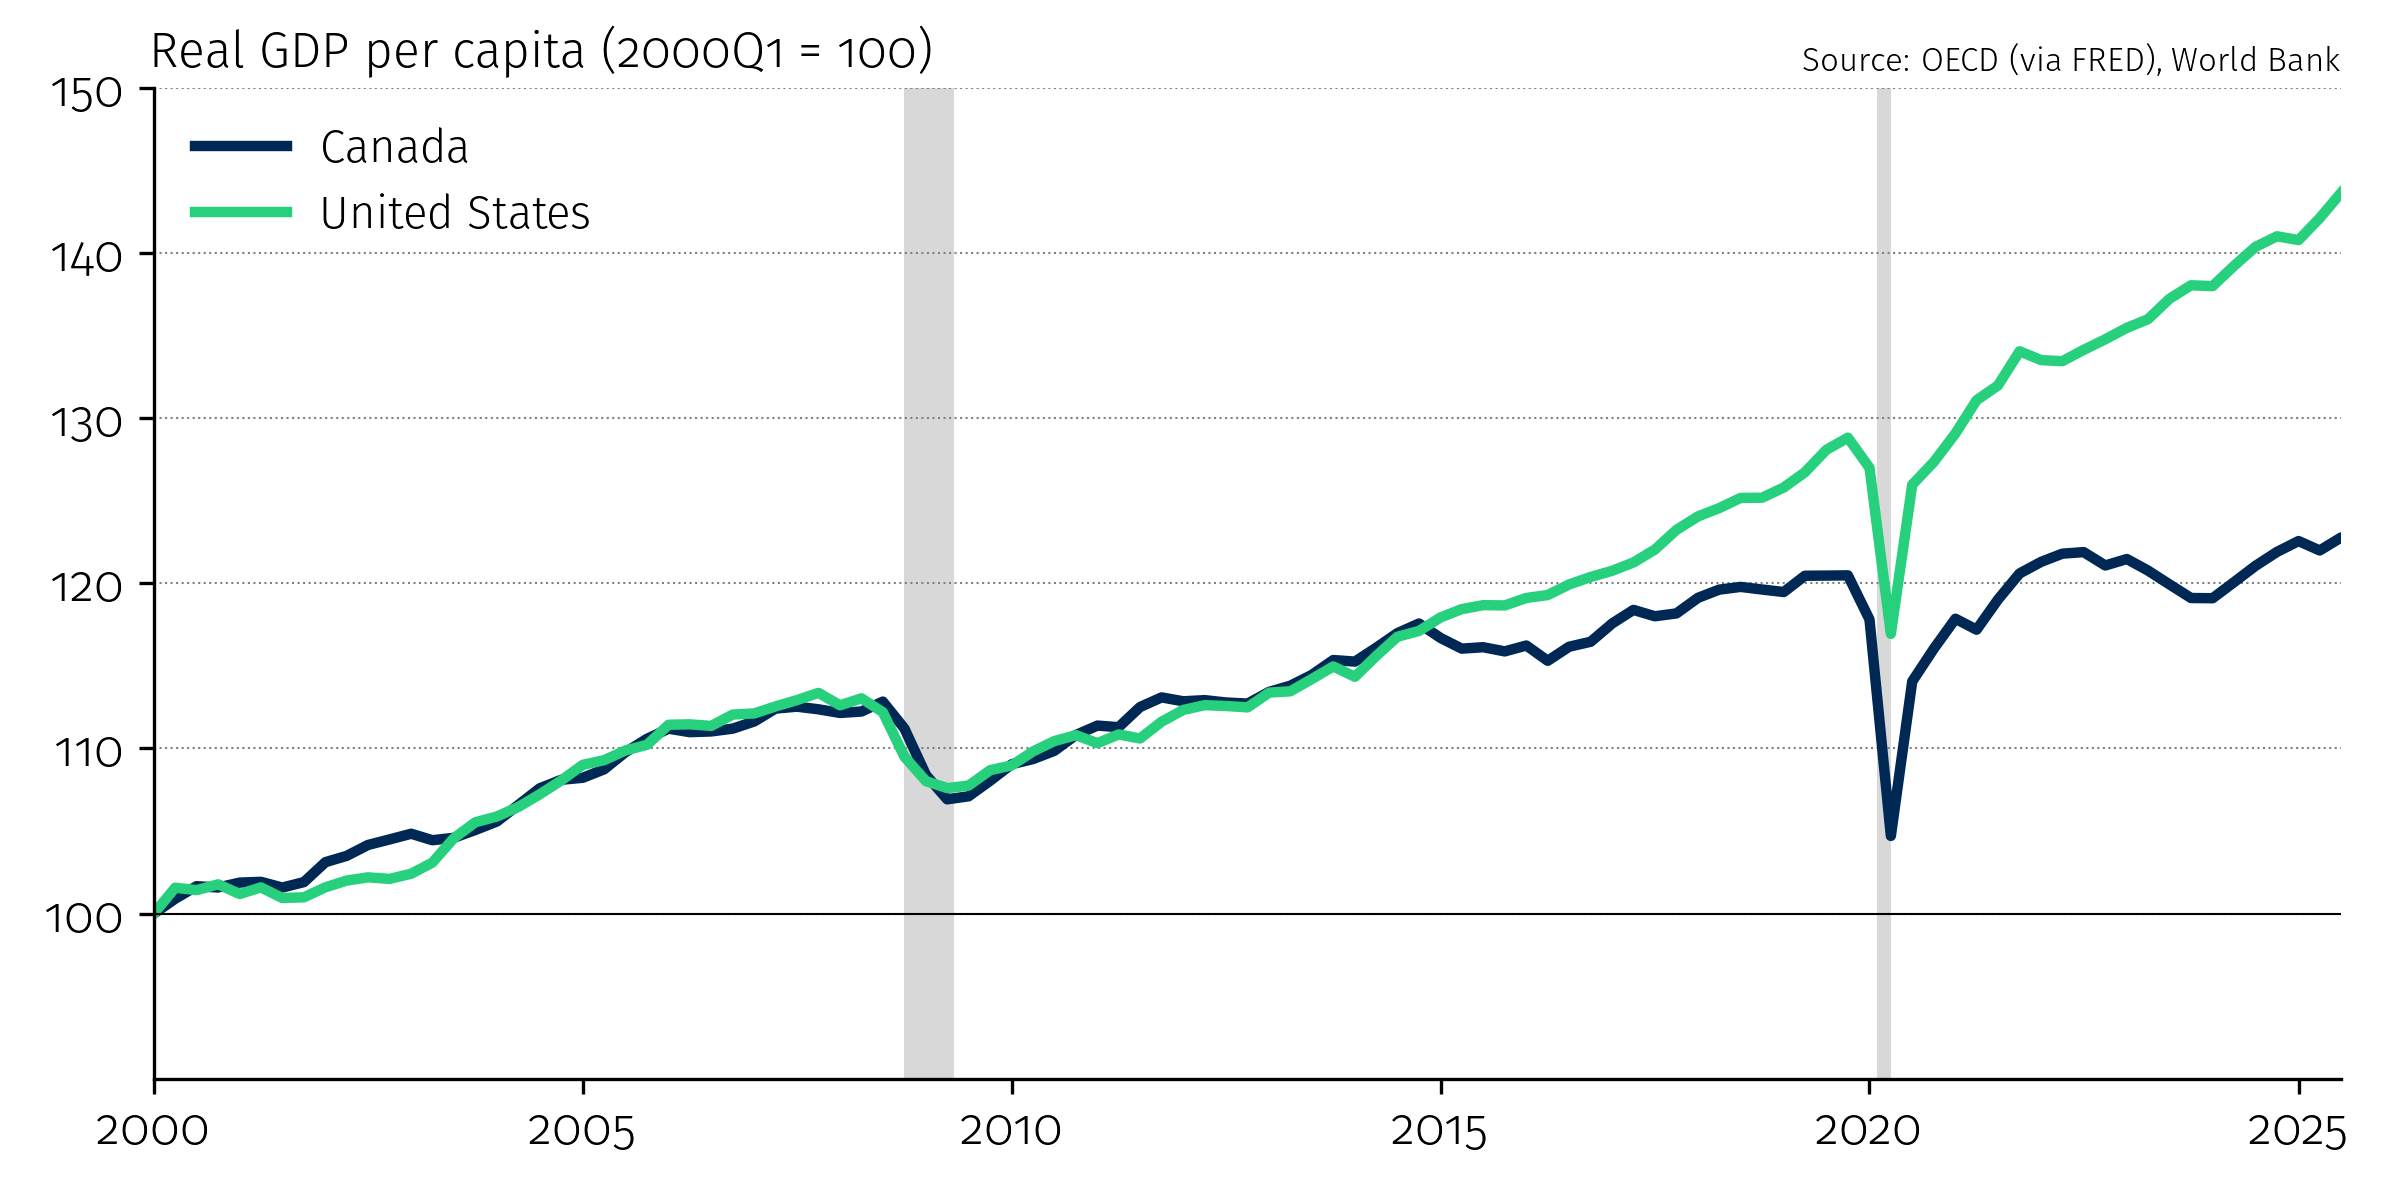
\includegraphics[width=0.95\textwidth, keepaspectratio]{gdp_per_capita_canada_usa.png}
   \end{figure}
\end{frame}

{
\setbeamertemplate{footline}{}
\begin{frame}{Le Canada a un problème de productivité}
   \begin{tikzpicture}[remember picture, overlay]
      \setcounter{newshl}{0}
      \newsheadline[globeandmail]{The Globe and Mail}{\guillemotleft~Productivity is an urgent problem for Canada. The response? A 15-year study~\guillemotright}
      \newsheadline[bloomberg]{Bloomberg}{\guillemotleft~Bank of Canada's Rogers Flags Weak Productivity `Emergency'~\guillemotright}
      \newsheadline[radiocanada]{Radio-Canada}{\guillemotleft~La productivité en chute fait craindre pour le niveau de vie des Canadiens~\guillemotright}
      \newsheadline[lapresse]{La Presse}{\guillemotleft~Urgence productivité : pourquoi notre niveau de vie prend le bord?~\guillemotright}
      \newsheadline[ledevoir]{Le Devoir}{\guillemotleft~Le très mauvais bilan du Canada et du Québec en matière de productivité~\guillemotright}
      \newsheadline[nationalpost]{National Post}{\guillemotleft~Businesses rank being `stifled by red tape' as more of a threat than Trump tariffs~\guillemotright}
   \end{tikzpicture}
\end{frame}
}

\begin{frame}[t]{Un problème de productivité?}
   \small
   Le PIB par habitant du Canada tire de la patte. Est-ce un problème de \textbf{productivité}?
   \vspace{0.2cm}

   \begin{defbox}[Deux mesures de la productivité]
      \vspace{-0.5cm}
      \begin{itemize}
         \setlength\itemsep{0.15cm}
         \item \textbf{Productivité du travail :} $Y / L = A^{\frac{1}{1 - \alpha}} \cdot (K / Y)^{\frac{\alpha}{1 - \alpha}}$
         
         Fonction de $A$ et de $K/Y$. Mesure la plus souvent citée dans les médias.

         \item \textbf{Productivité totale des facteurs (PTF) :} $A$

         L'efficacité \guillemotleft~pure~\guillemotright\ avec laquelle on combine $K$ et $L$
      \end{itemize}
   \end{defbox}
   \vspace{0.1cm}
   \begin{keyinsight}[Rappel]
      On peut décomposer le PIB par habitant: $Y / N = (Y / L) \cdot (L / N)$. Où est le problème?
   \end{keyinsight}
\end{frame}

\begin{frame}{Décomposition de la croissance canadienne}
   \begin{figure}
      \centering
      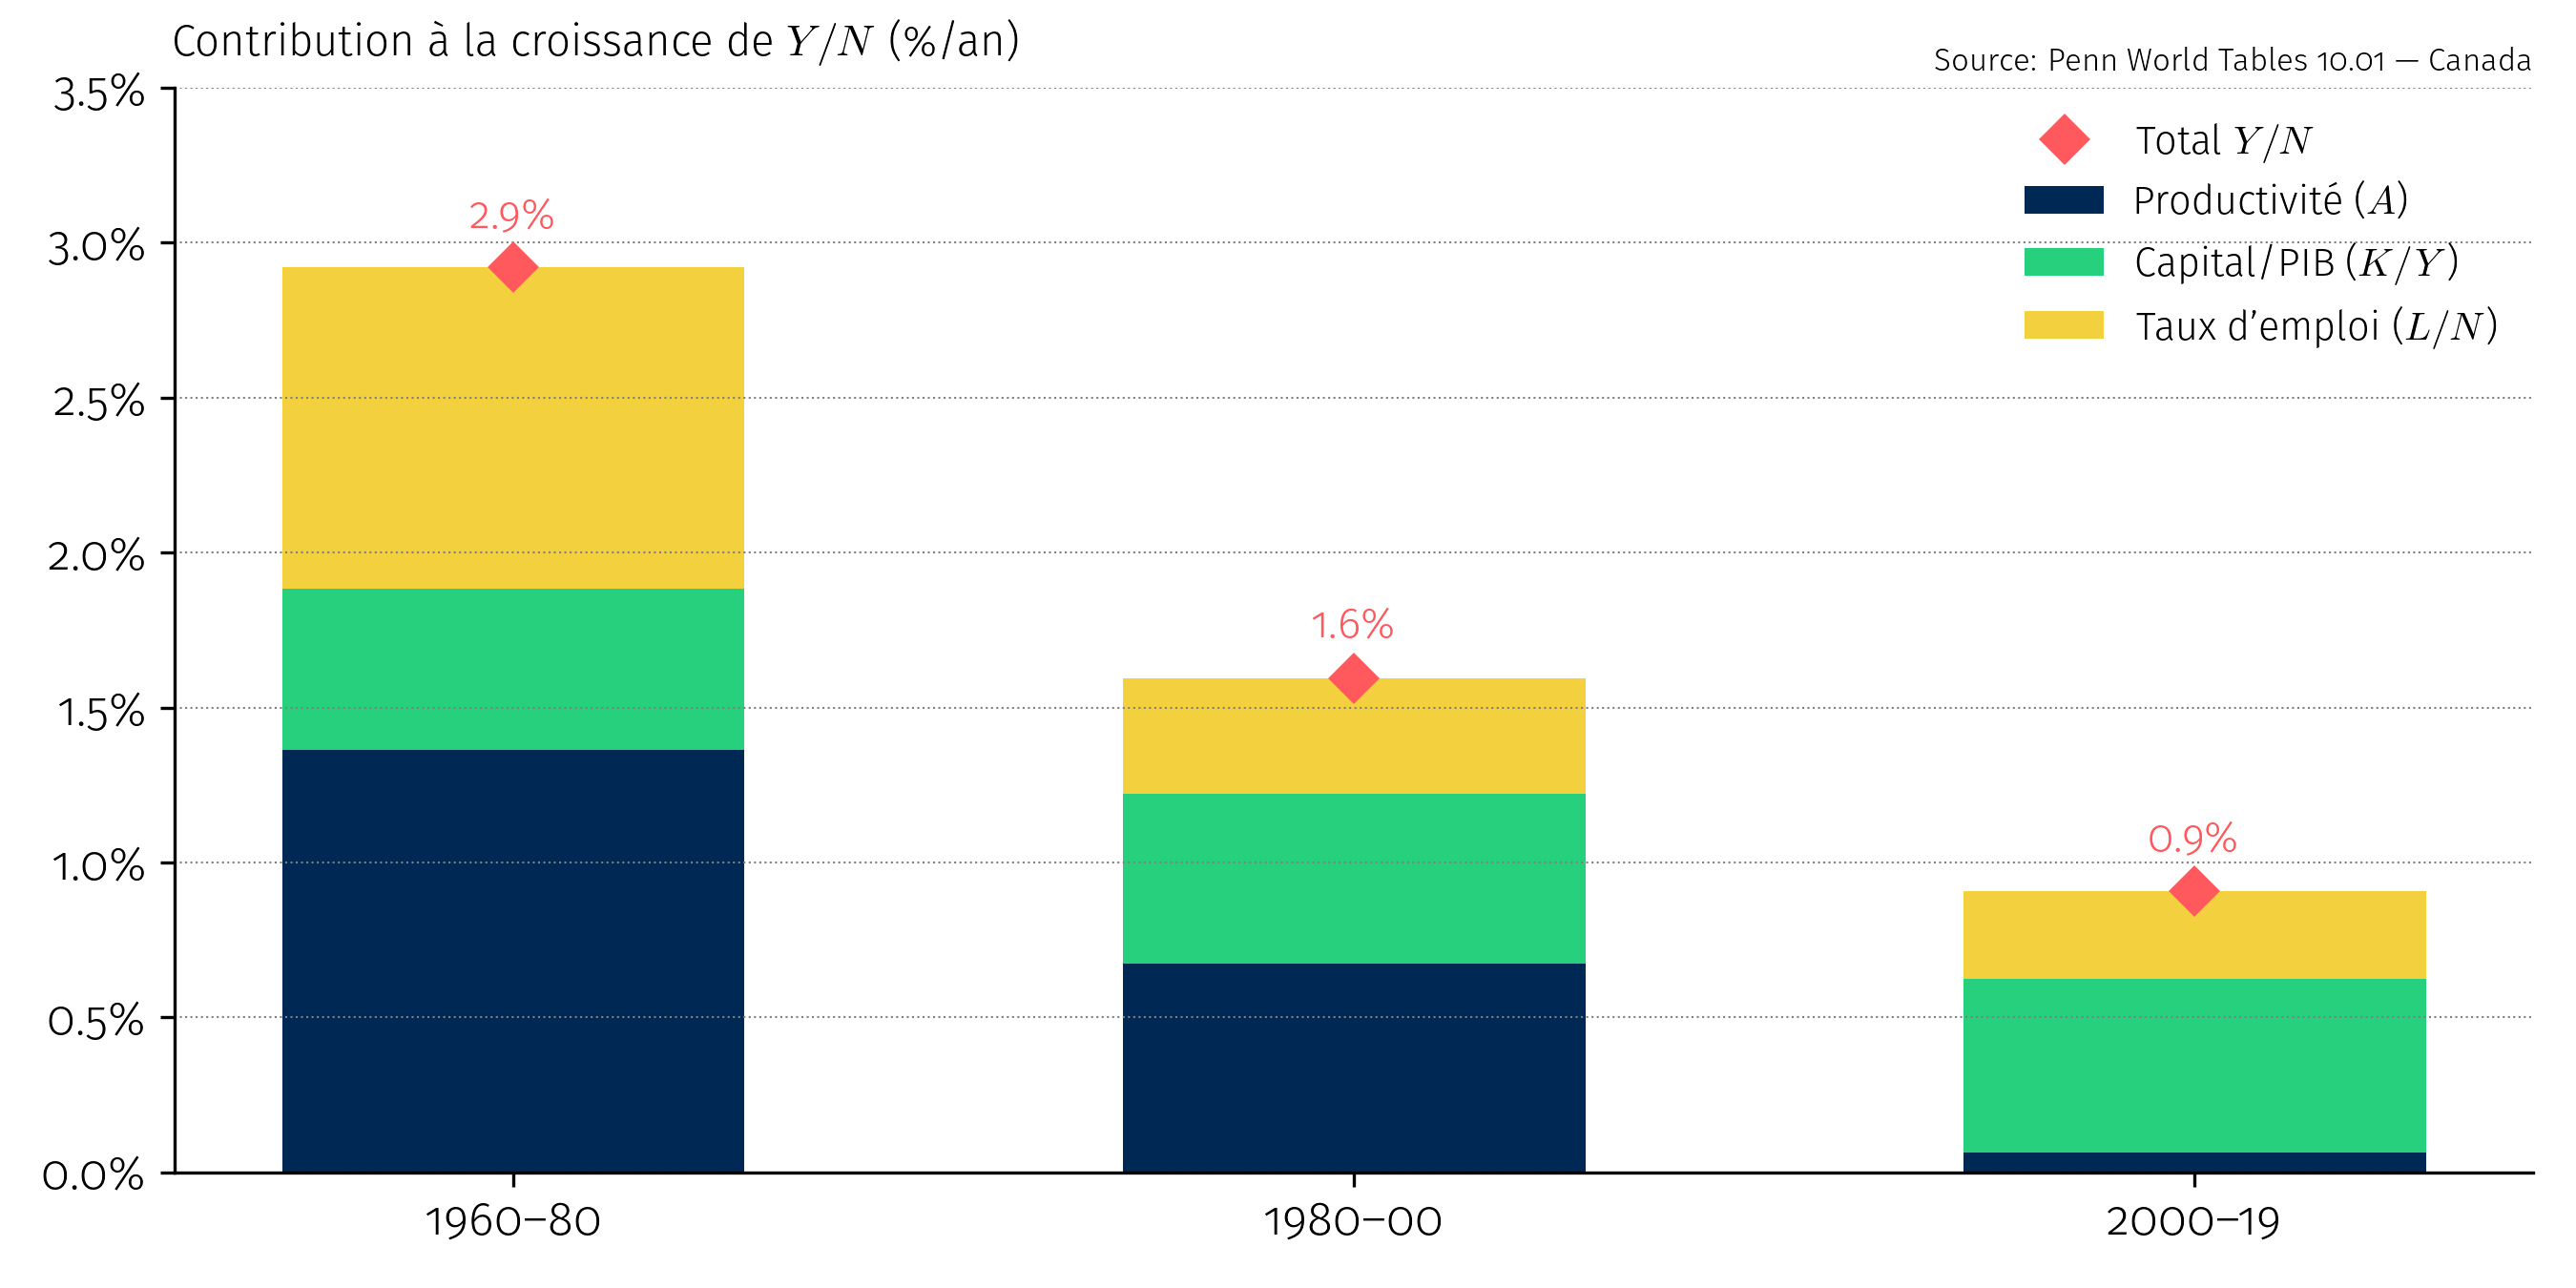
\includegraphics[width=0.95\textwidth, keepaspectratio]{canada_gdp_decomposition.png}
   \end{figure}
\end{frame}

\begin{frame}{Le Canada en comparaison internationale}
   \begin{figure}
      \centering
      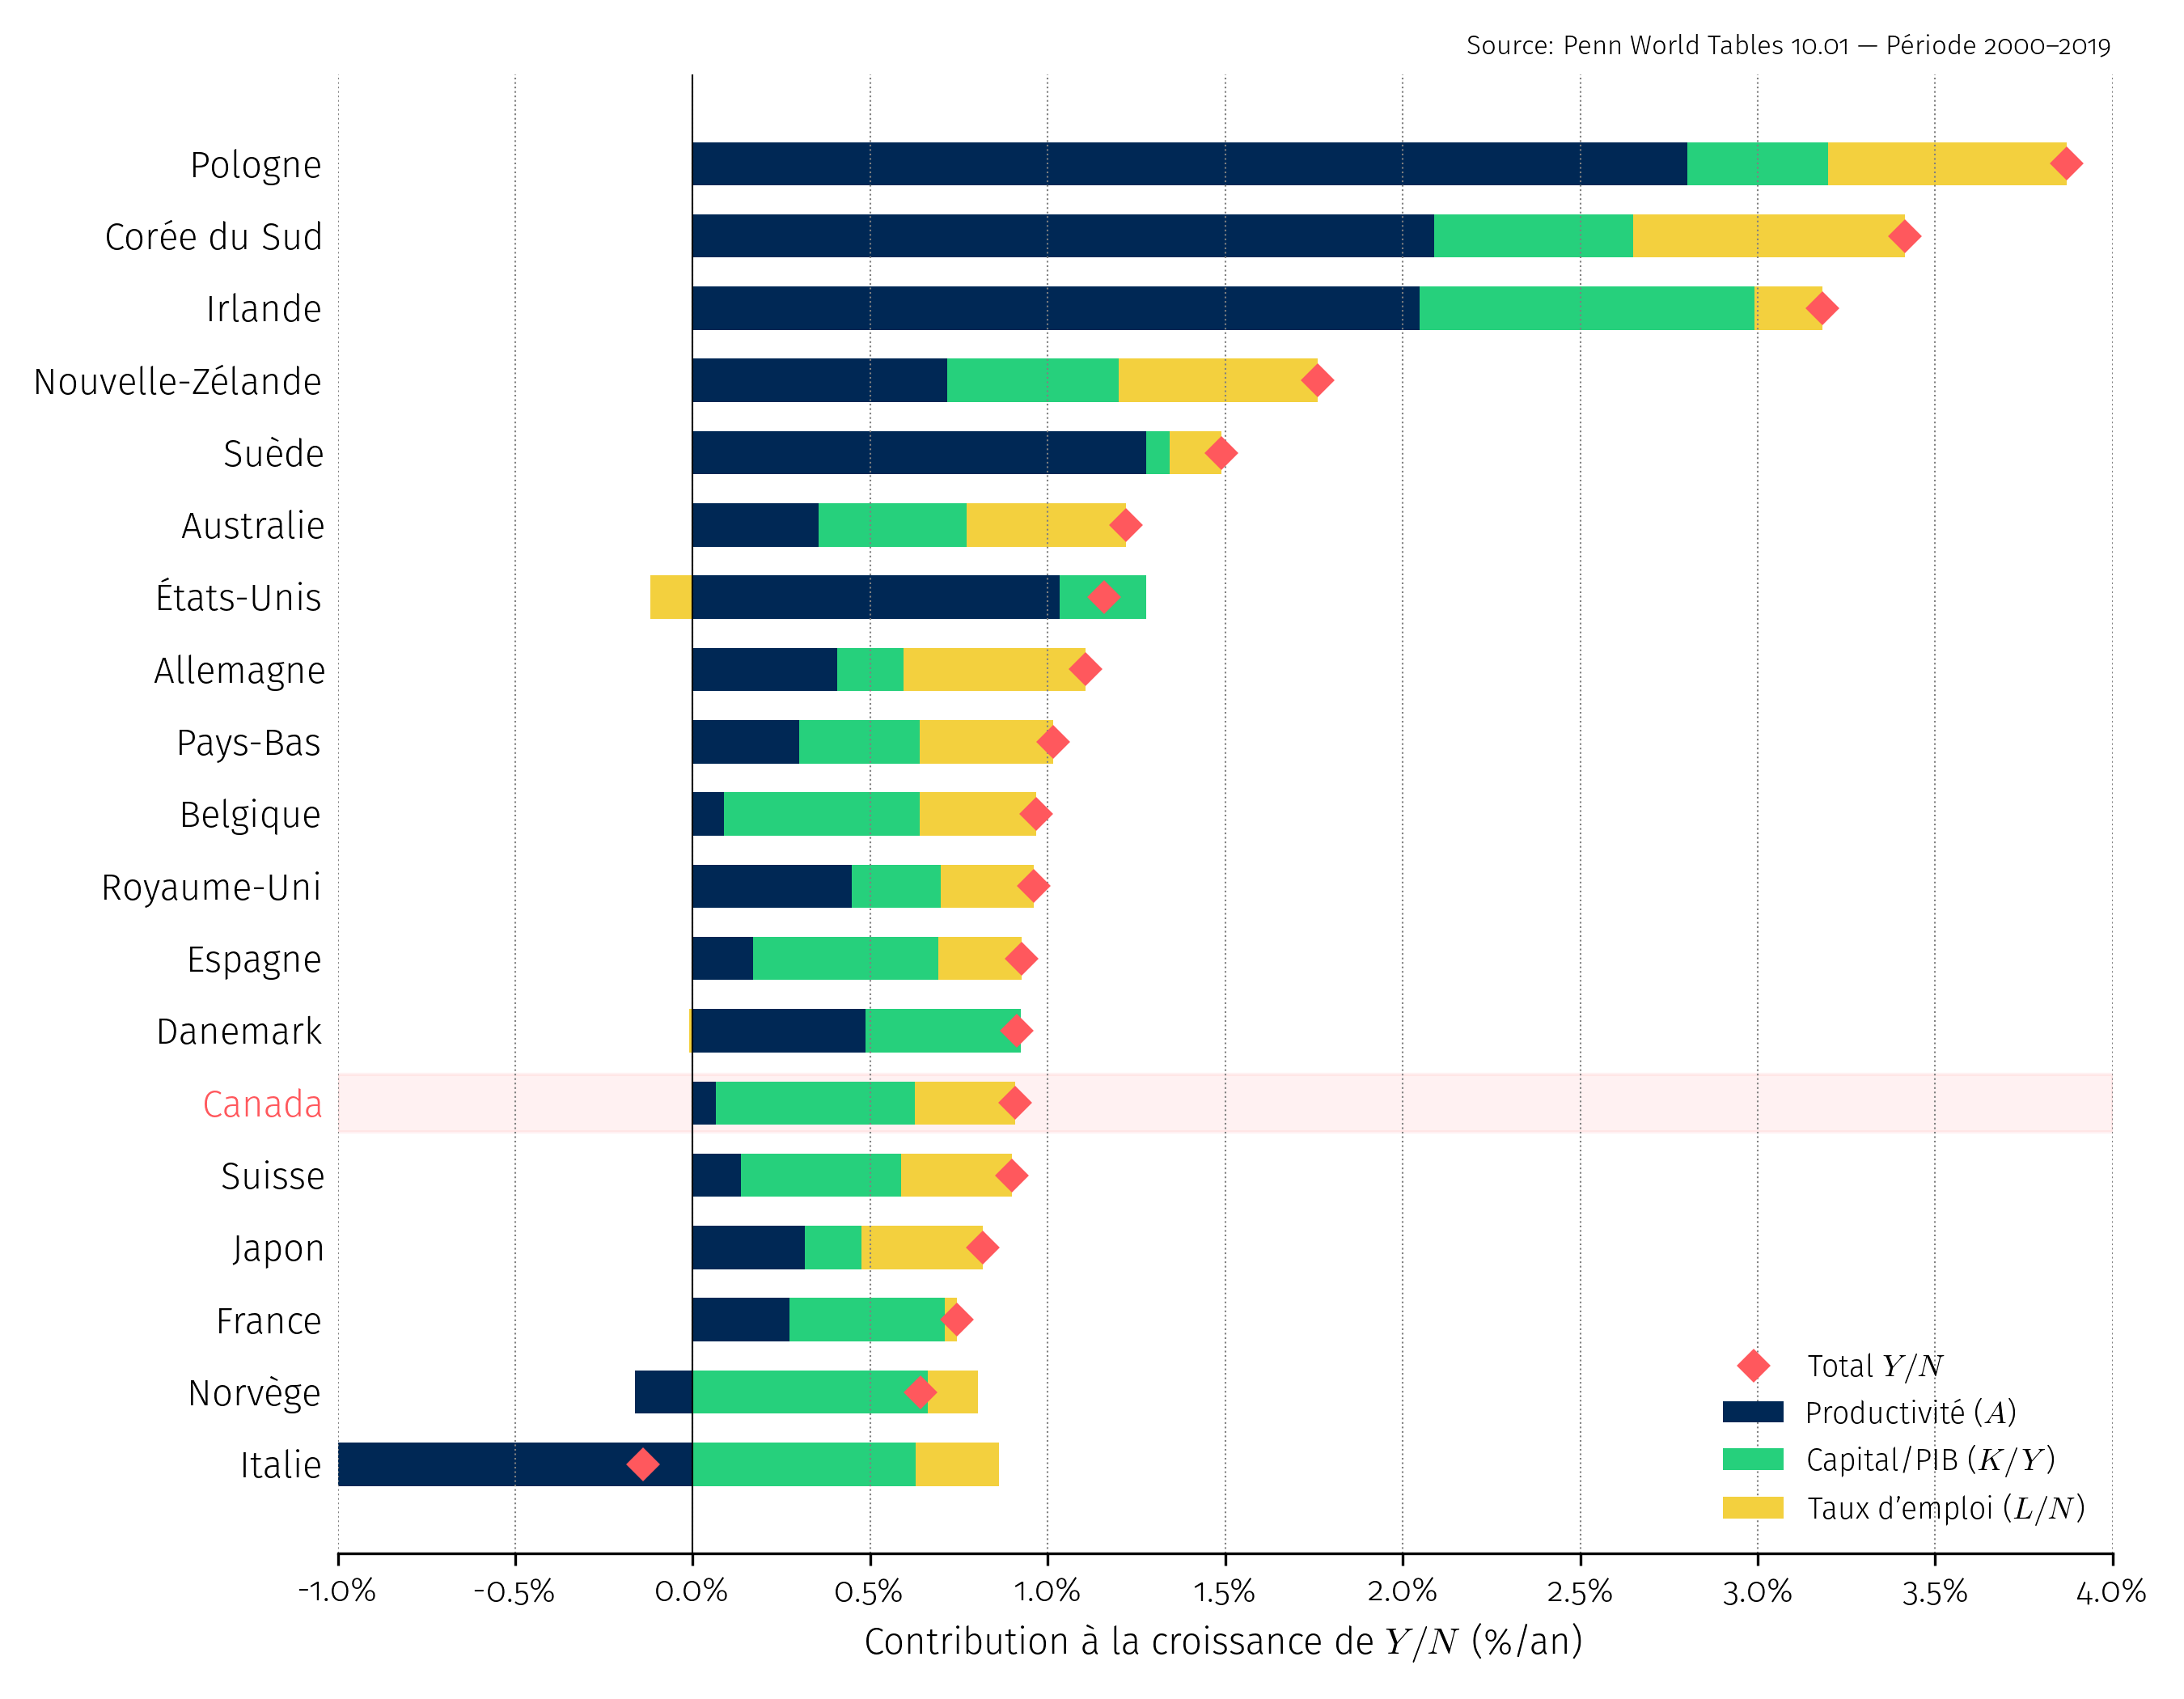
\includegraphics[width=0.95\textwidth, height=0.82\textheight, keepaspectratio]{canada_gdp_decomposition_countries.png}
   \end{figure}
\end{frame}

\begin{frame}{La productivité explique $\sim$50\,\% des écarts de revenus entre pays}
   \begin{figure}
      \centering
      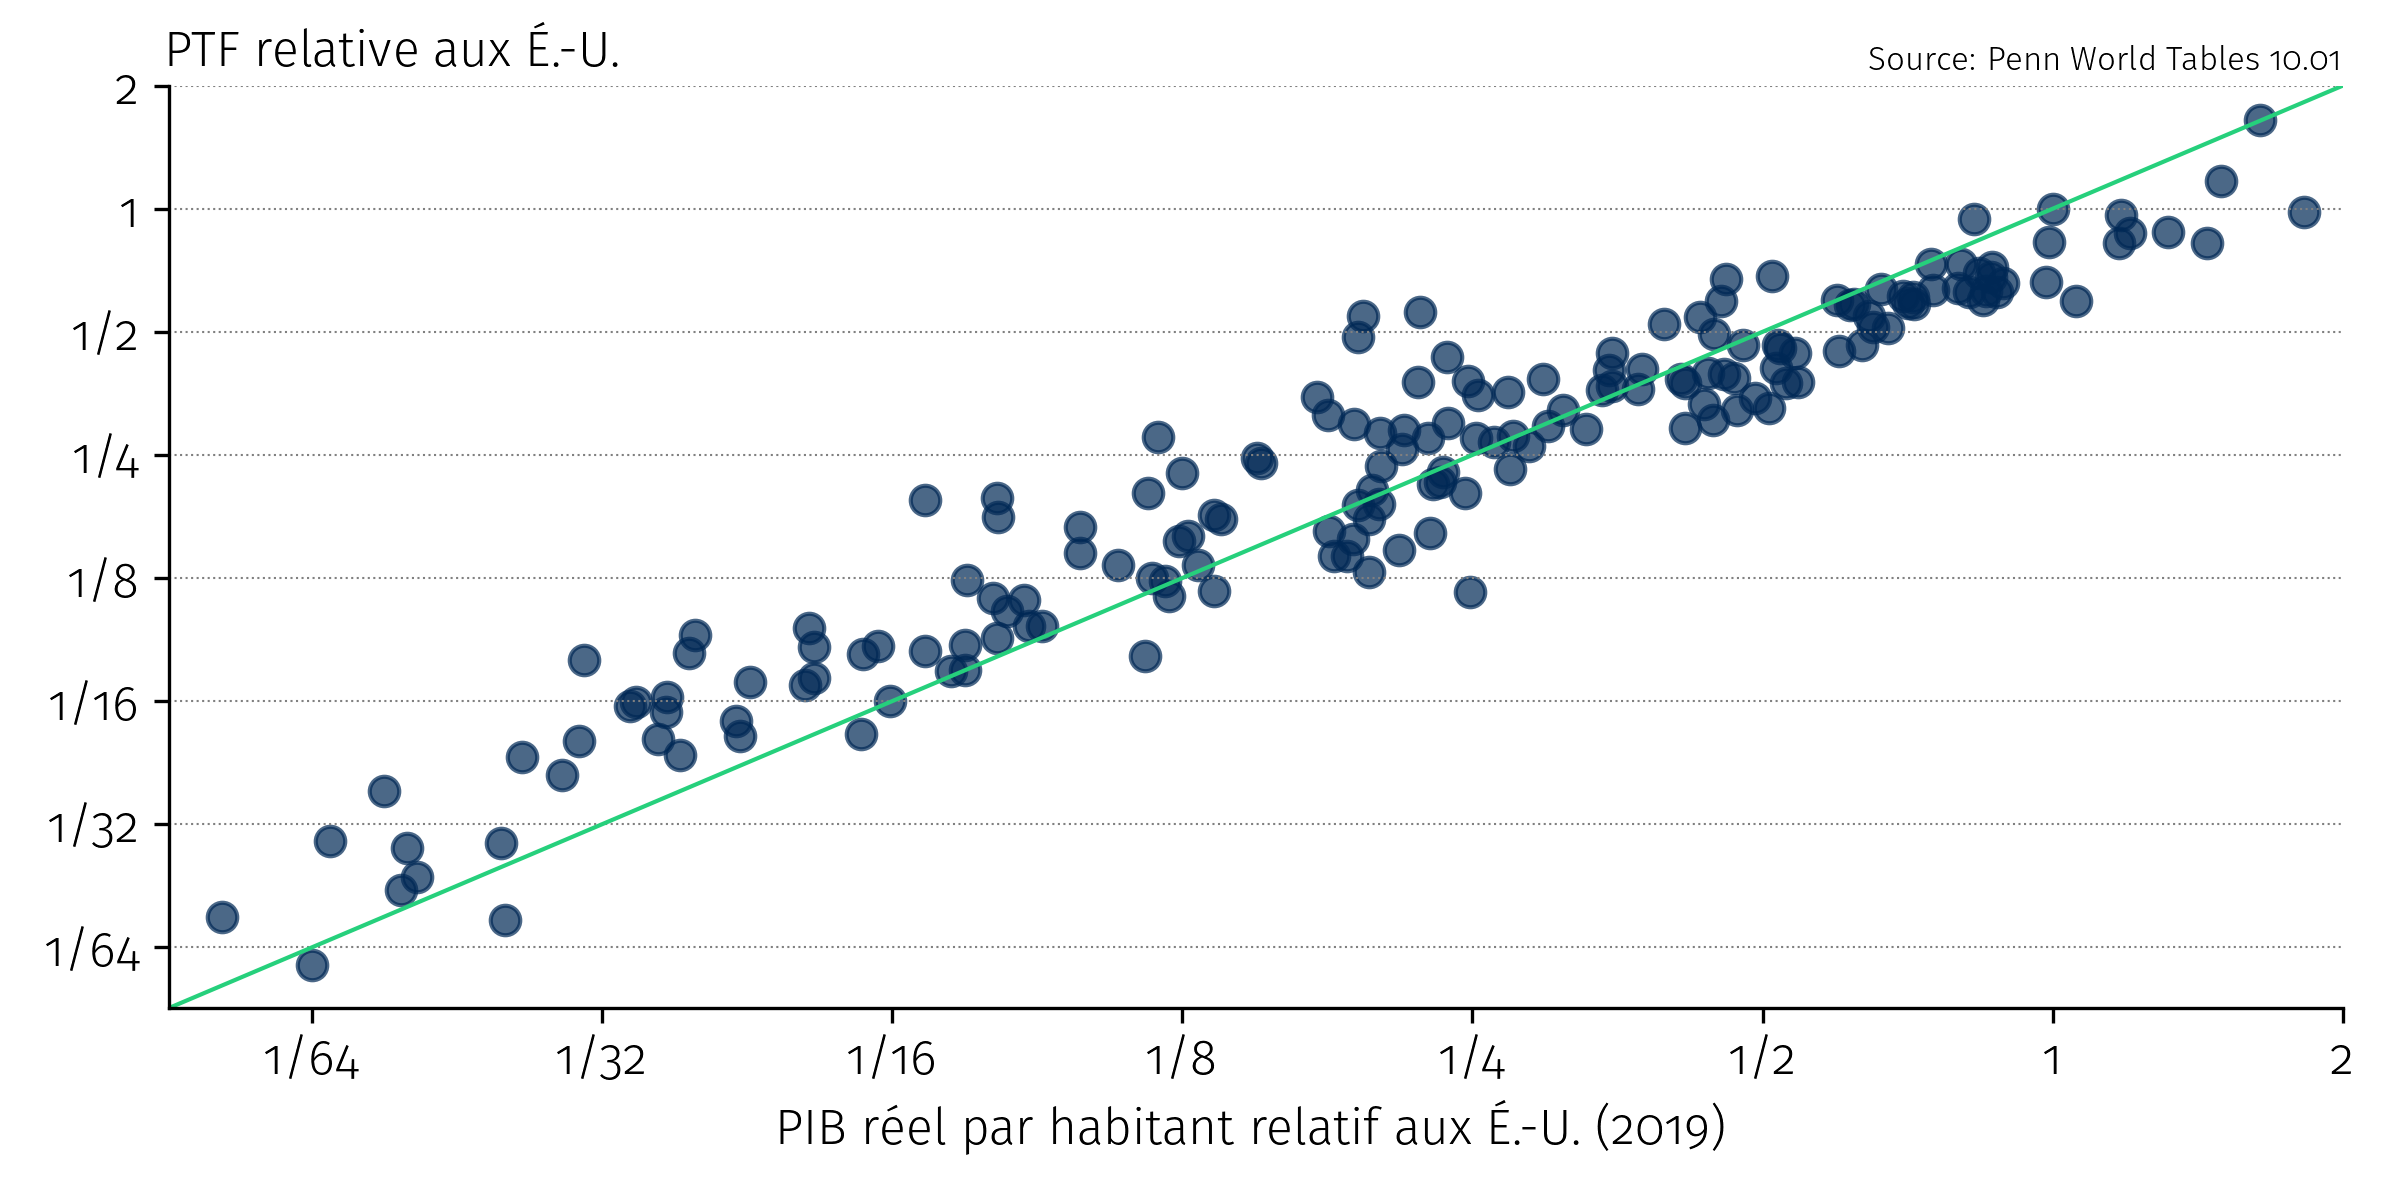
\includegraphics[width=0.95\textwidth]{development_accounting_tfp.png}
   \end{figure}
\end{frame}

\begin{frame}{Qu'est-ce qui se cache derrière la PTF\,?}
   \vspace{0.8cm}
   \centering
   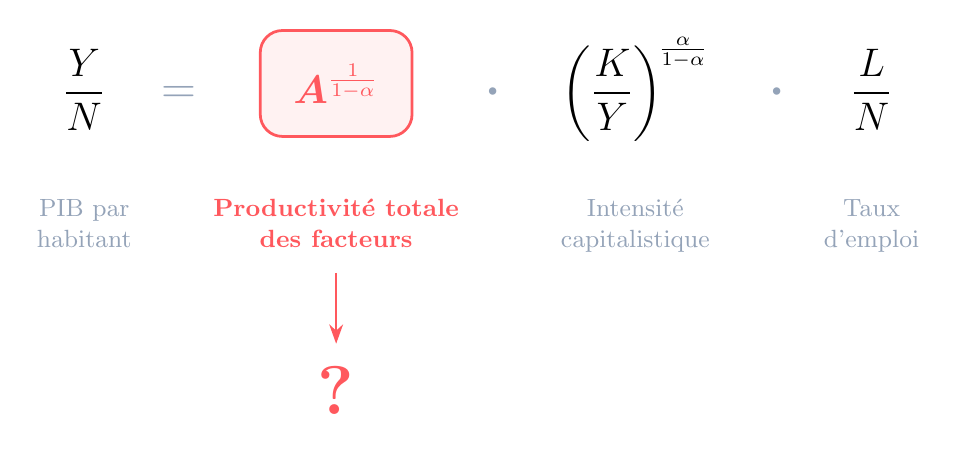
\begin{tikzpicture}[
      op/.style={font=\LARGE, text=HECgray},
      lbl/.style={font=\small, text=HECgray, align=center},
   ]
      % Y/N
      \node[anchor=base] (yn) at (0,0) {\Large$\dfrac{Y}{N}$};
      \node[lbl, anchor=north] at (0,-1.1) {PIB par\\habitant};

      % =
      \node[anchor=base, op] at (1.2,0) {$=$};

      % A (highlighted)
      \node[anchor=base, rounded corners=8pt, fill=HECcoral!8, draw=HECcoral,
            line width=1pt, inner sep=12pt] (A) at (3.2,0)
         {\Large\textcolor{HECcoral}{$\bm{A}^{\frac{1}{1-\alpha}}$}};
      \node[lbl, anchor=north, text=HECcoral, font=\small\bfseries] (lA) at (3.2,-1.1)
         {Productivité totale\\des facteurs};

      % ·
      \node[anchor=base, op] at (5.2,0) {$\boldsymbol{\cdot}$};

      % (K/Y)^(α/(1-α))
      \node[anchor=base] (ky) at (7.0,0) {\Large$\left(\dfrac{K}{Y}\right)^{\!\frac{\alpha}{1-\alpha}}$};
      \node[lbl, anchor=north] at (7.0,-1.1) {Intensité\\capitalistique};

      % ·
      \node[anchor=base, op] at (8.8,0) {$\boldsymbol{\cdot}$};

      % L/N
      \node[anchor=base] (ln) at (10.0,0) {\Large$\dfrac{L}{N}$};
      \node[lbl, anchor=north] at (10.0,-1.1) {Taux\\d'emploi};

      % Downward arrow from A
      \draw[-{Stealth[length=7pt, width=5pt]}, line width=0.8pt, HECcoral]
         ([yshift=-0.2cm]lA.south) -- ++(0,-0.9cm);

      % Question mark
      \node[font=\fontsize{36}{42}\selectfont\bfseries, text=HECcoral]
         at ([yshift=-1.7cm]lA.south) {?};
   \end{tikzpicture}
\end{frame}

% ============================================================================
\begin{frame}{Plan}
   \begin{enumerate}
      \setlength\itemsep{0.5cm}
      \item \textbf{Théories de la productivité}
      \item Indicateurs du marché du travail
      \item Un modèle simple du marché du travail
      \item Applications du modèle
      \item Technologie, IA, et inégalités
   \end{enumerate}
\end{frame}

% ============================================================================
\sectionframe{Théories de la productivité}
% ============================================================================

\begin{frame}{Théories de la PTF}
   \begin{enumerate}
      \setlength\itemsep{0.5cm}
      \item \textbf{Technologie et idées}
      \item Géographie, climat, et culture
      \item Capital humain
      \item Institutions
   \end{enumerate}
\end{frame}

% --- 1. Technologie et idées ------------------------------------------------

\begin{frame}{La croissance coïncide avec les nouvelles idées}
   \begin{figure}
      \centering
      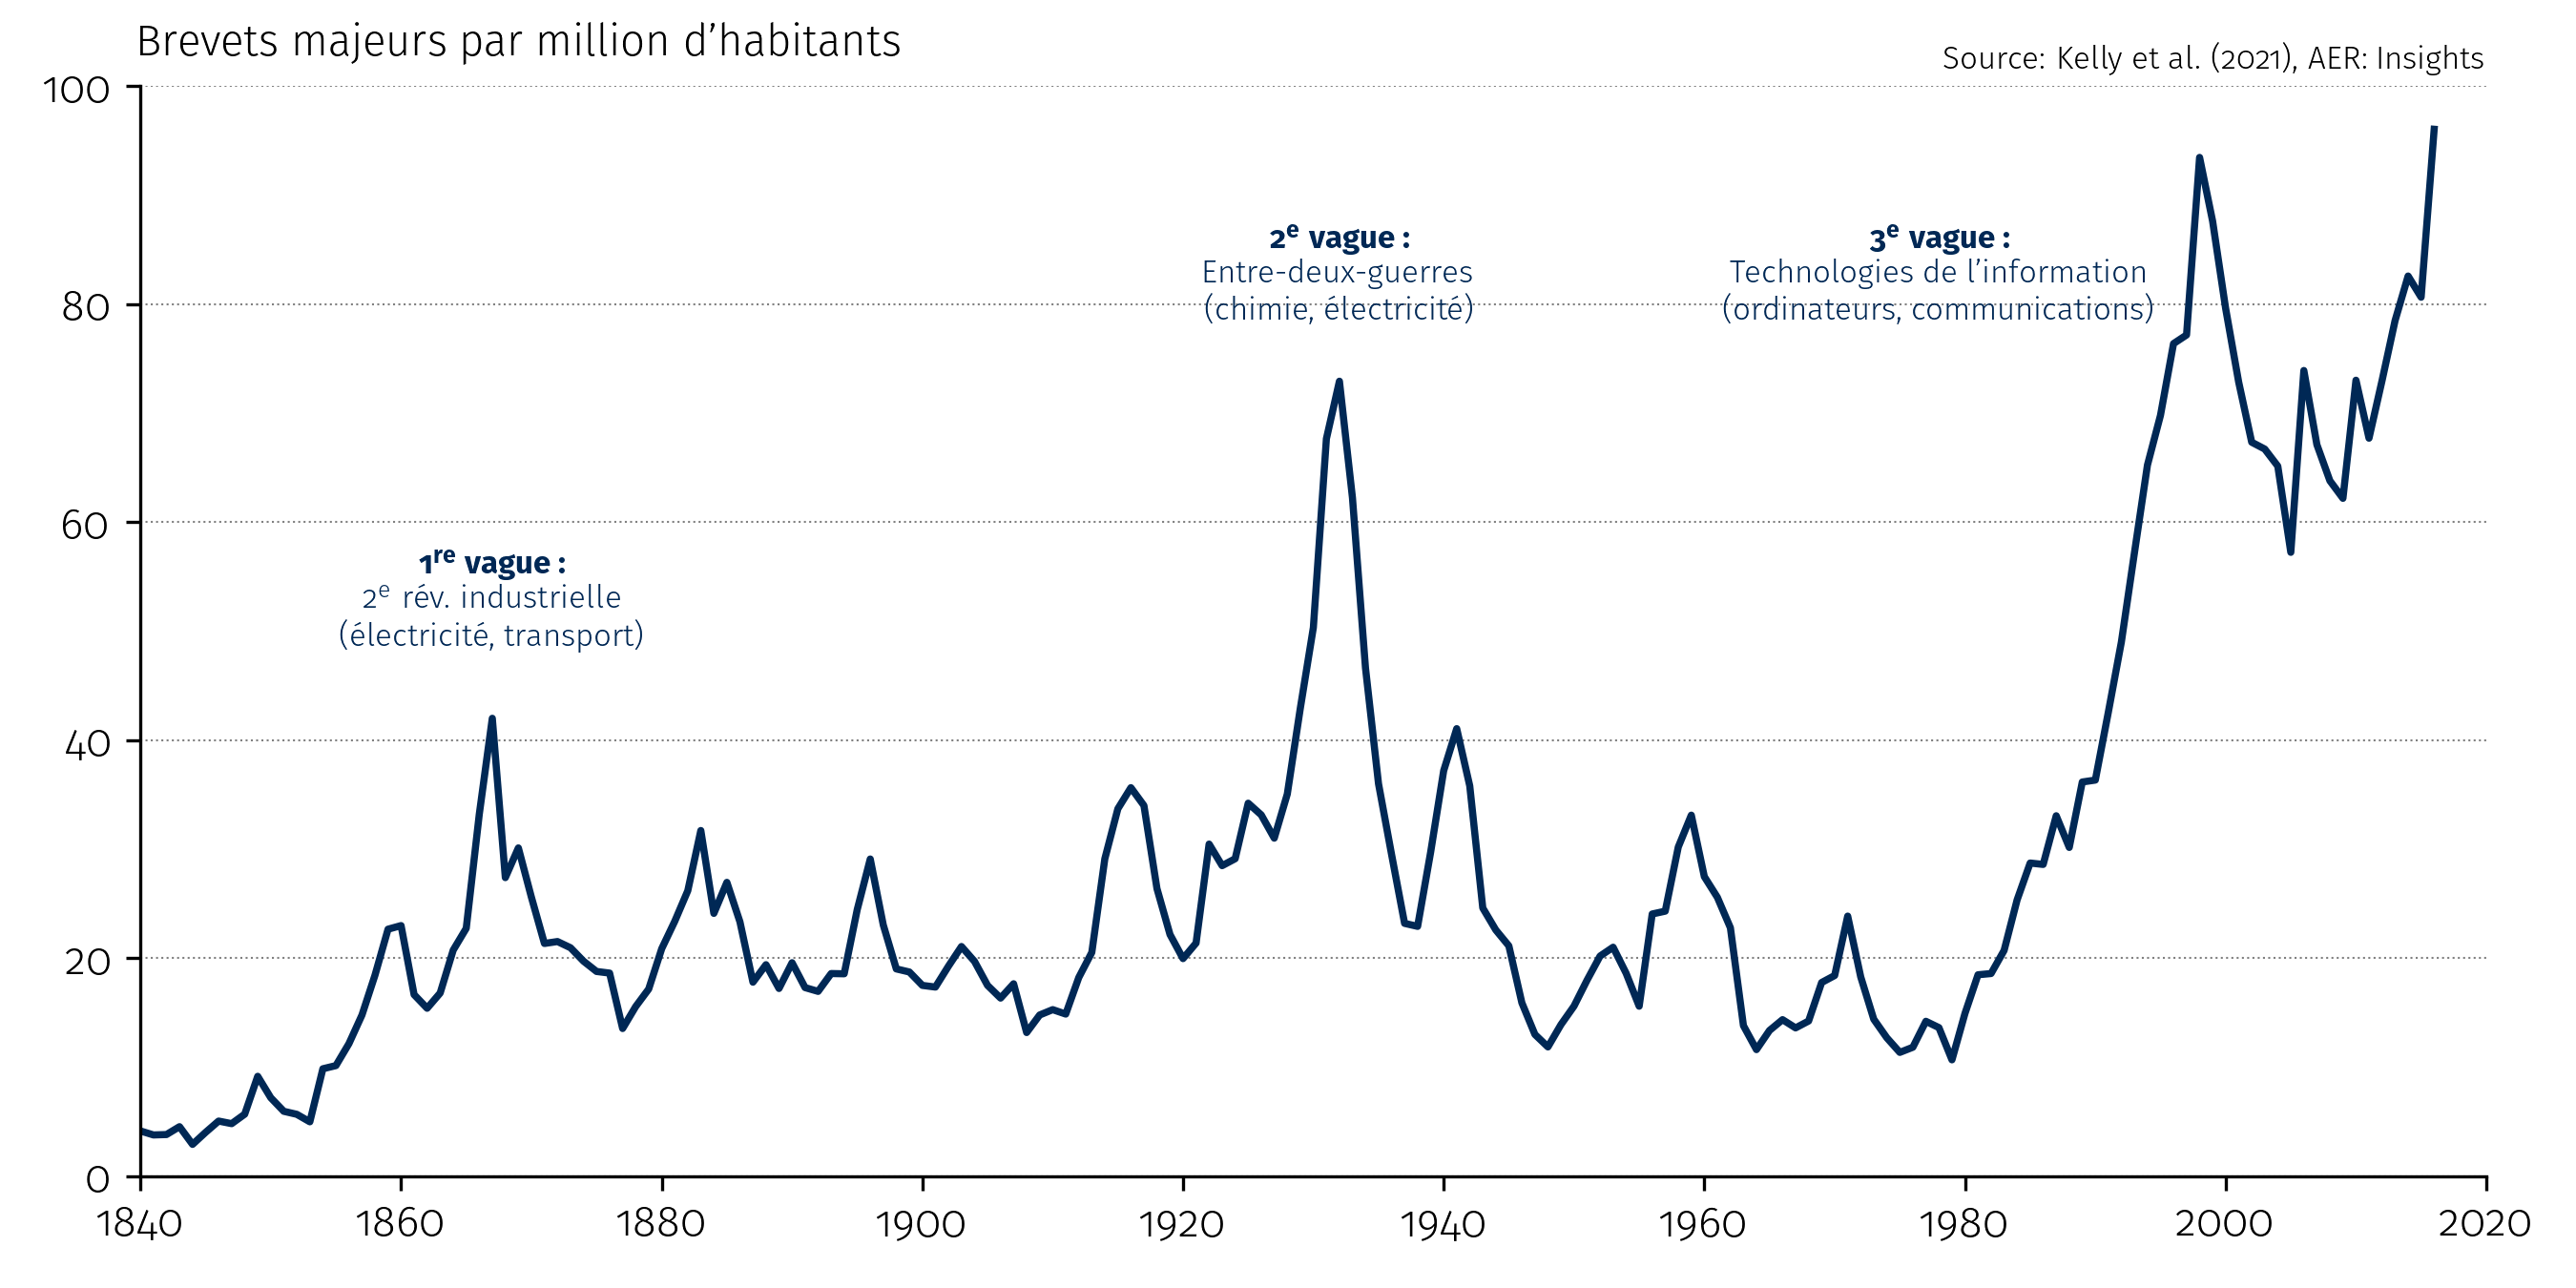
\includegraphics[width=0.95\textwidth]{kelly_et_al_2021.png}
   \end{figure}
\end{frame}

\begin{frame}[t]{L'innovation n'est pas un accident}
   \begin{figure}
      \centering
      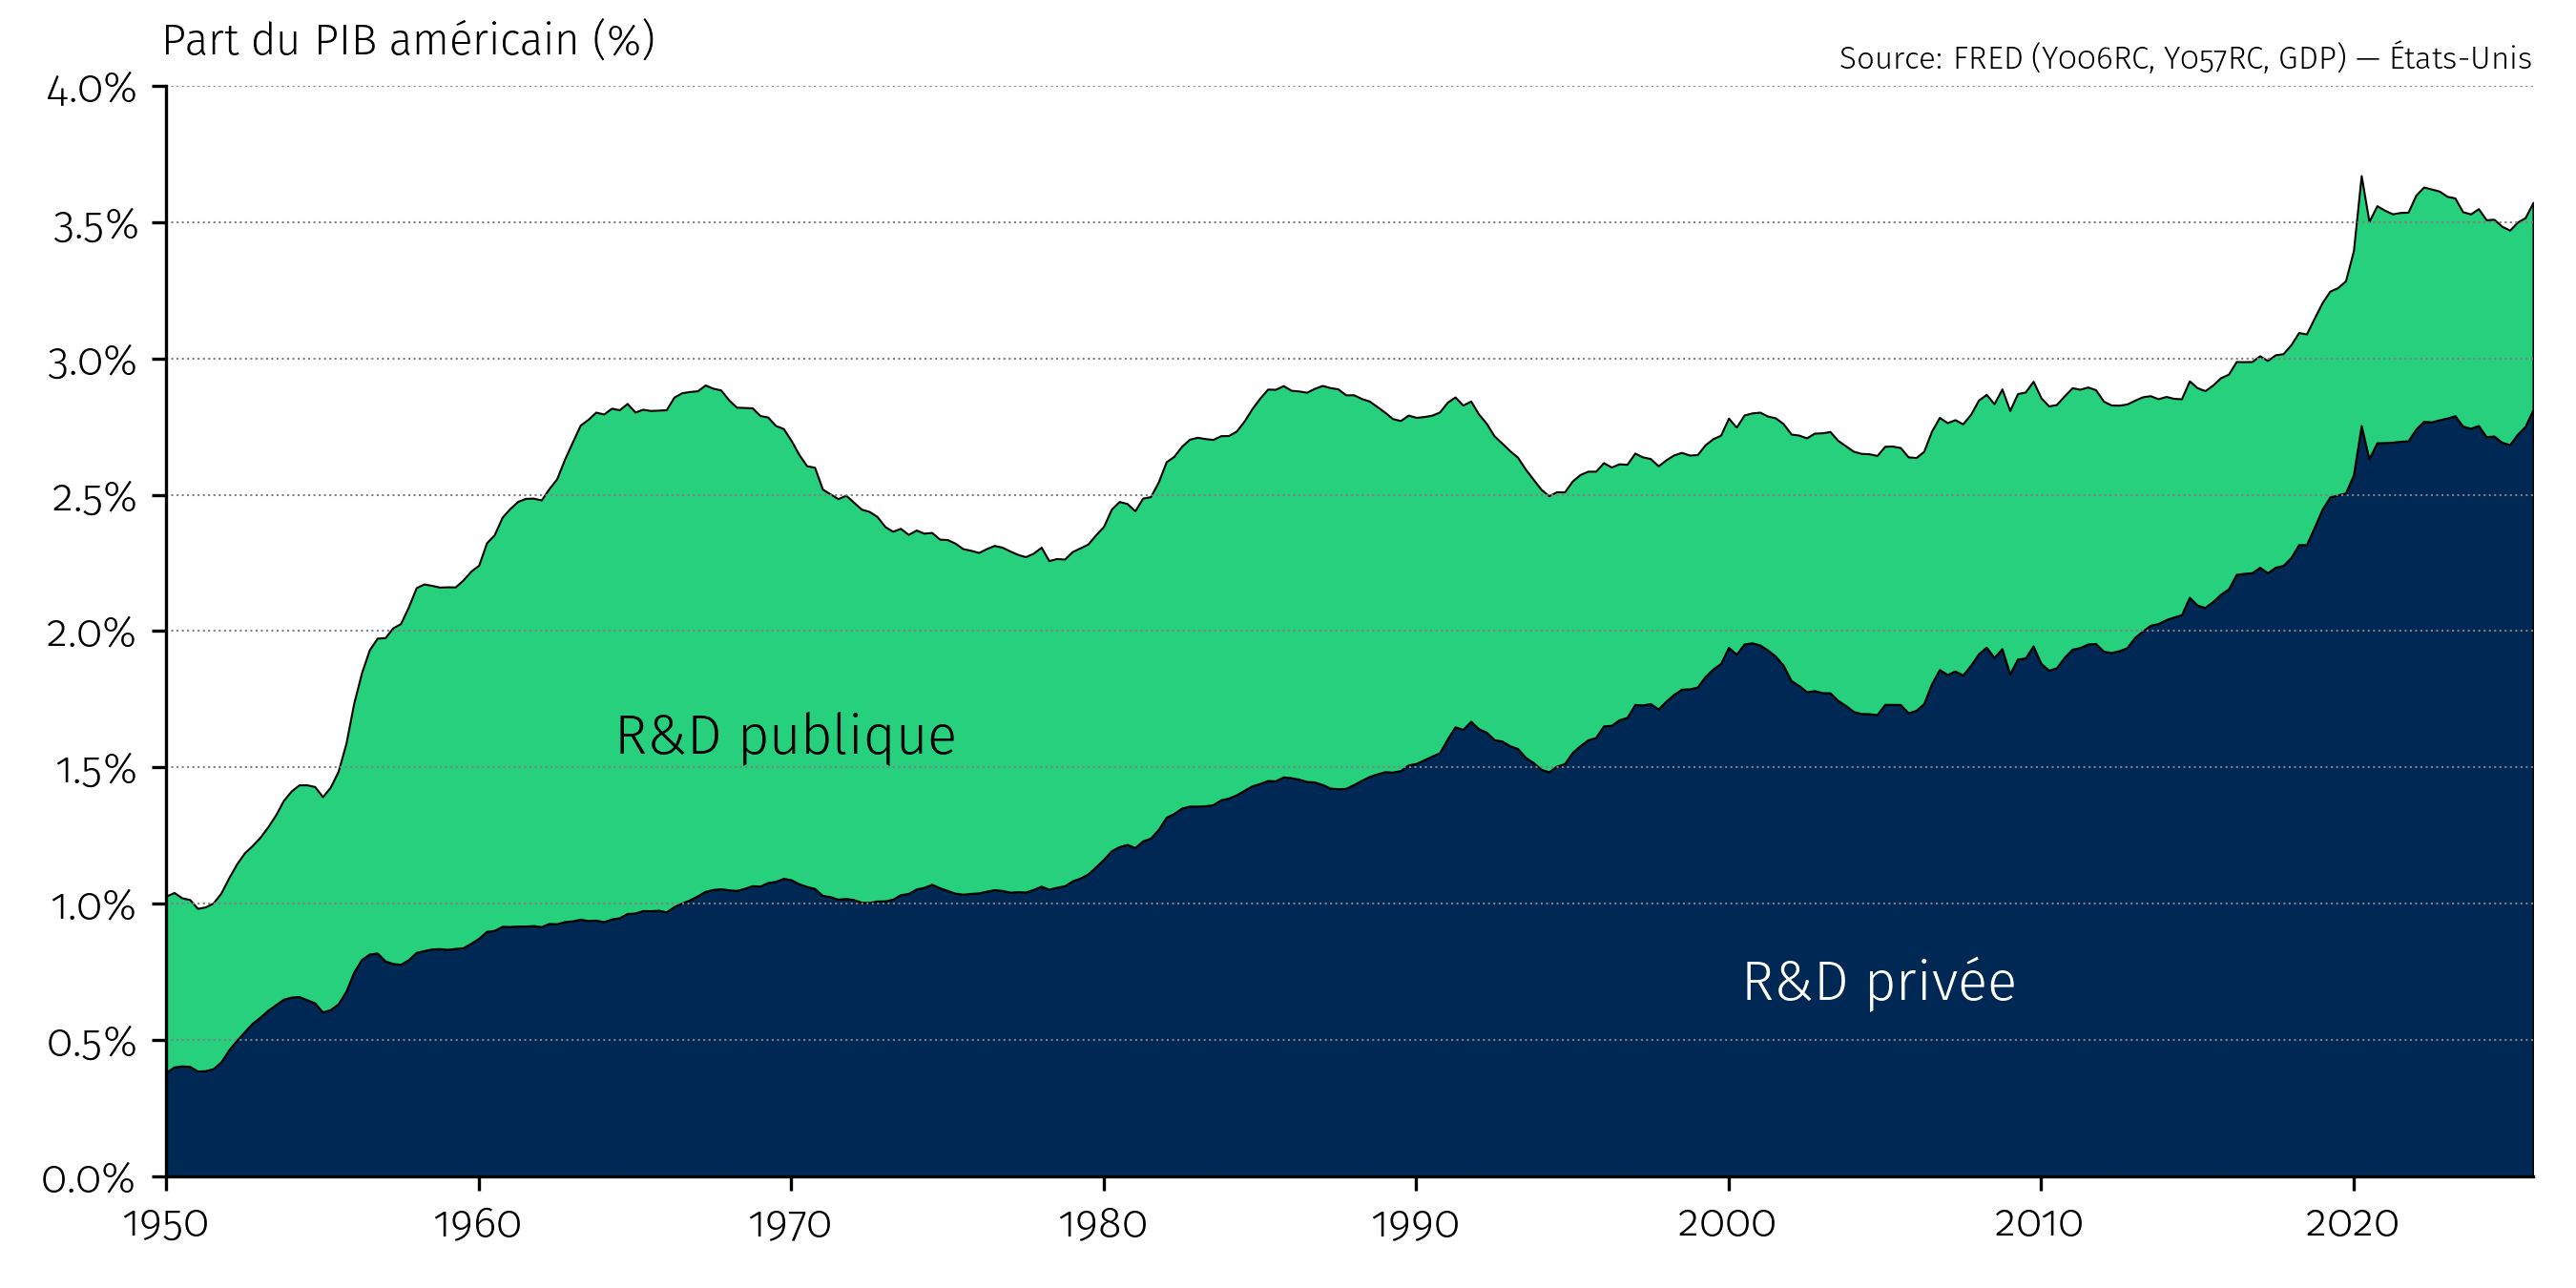
\includegraphics[width=0.95\textwidth, keepaspectratio]{rd_gdp_share.png}
   \end{figure}
\end{frame}

\begin{frame}{La R\&D est un effort mondial}
   \begin{figure}
      \centering
      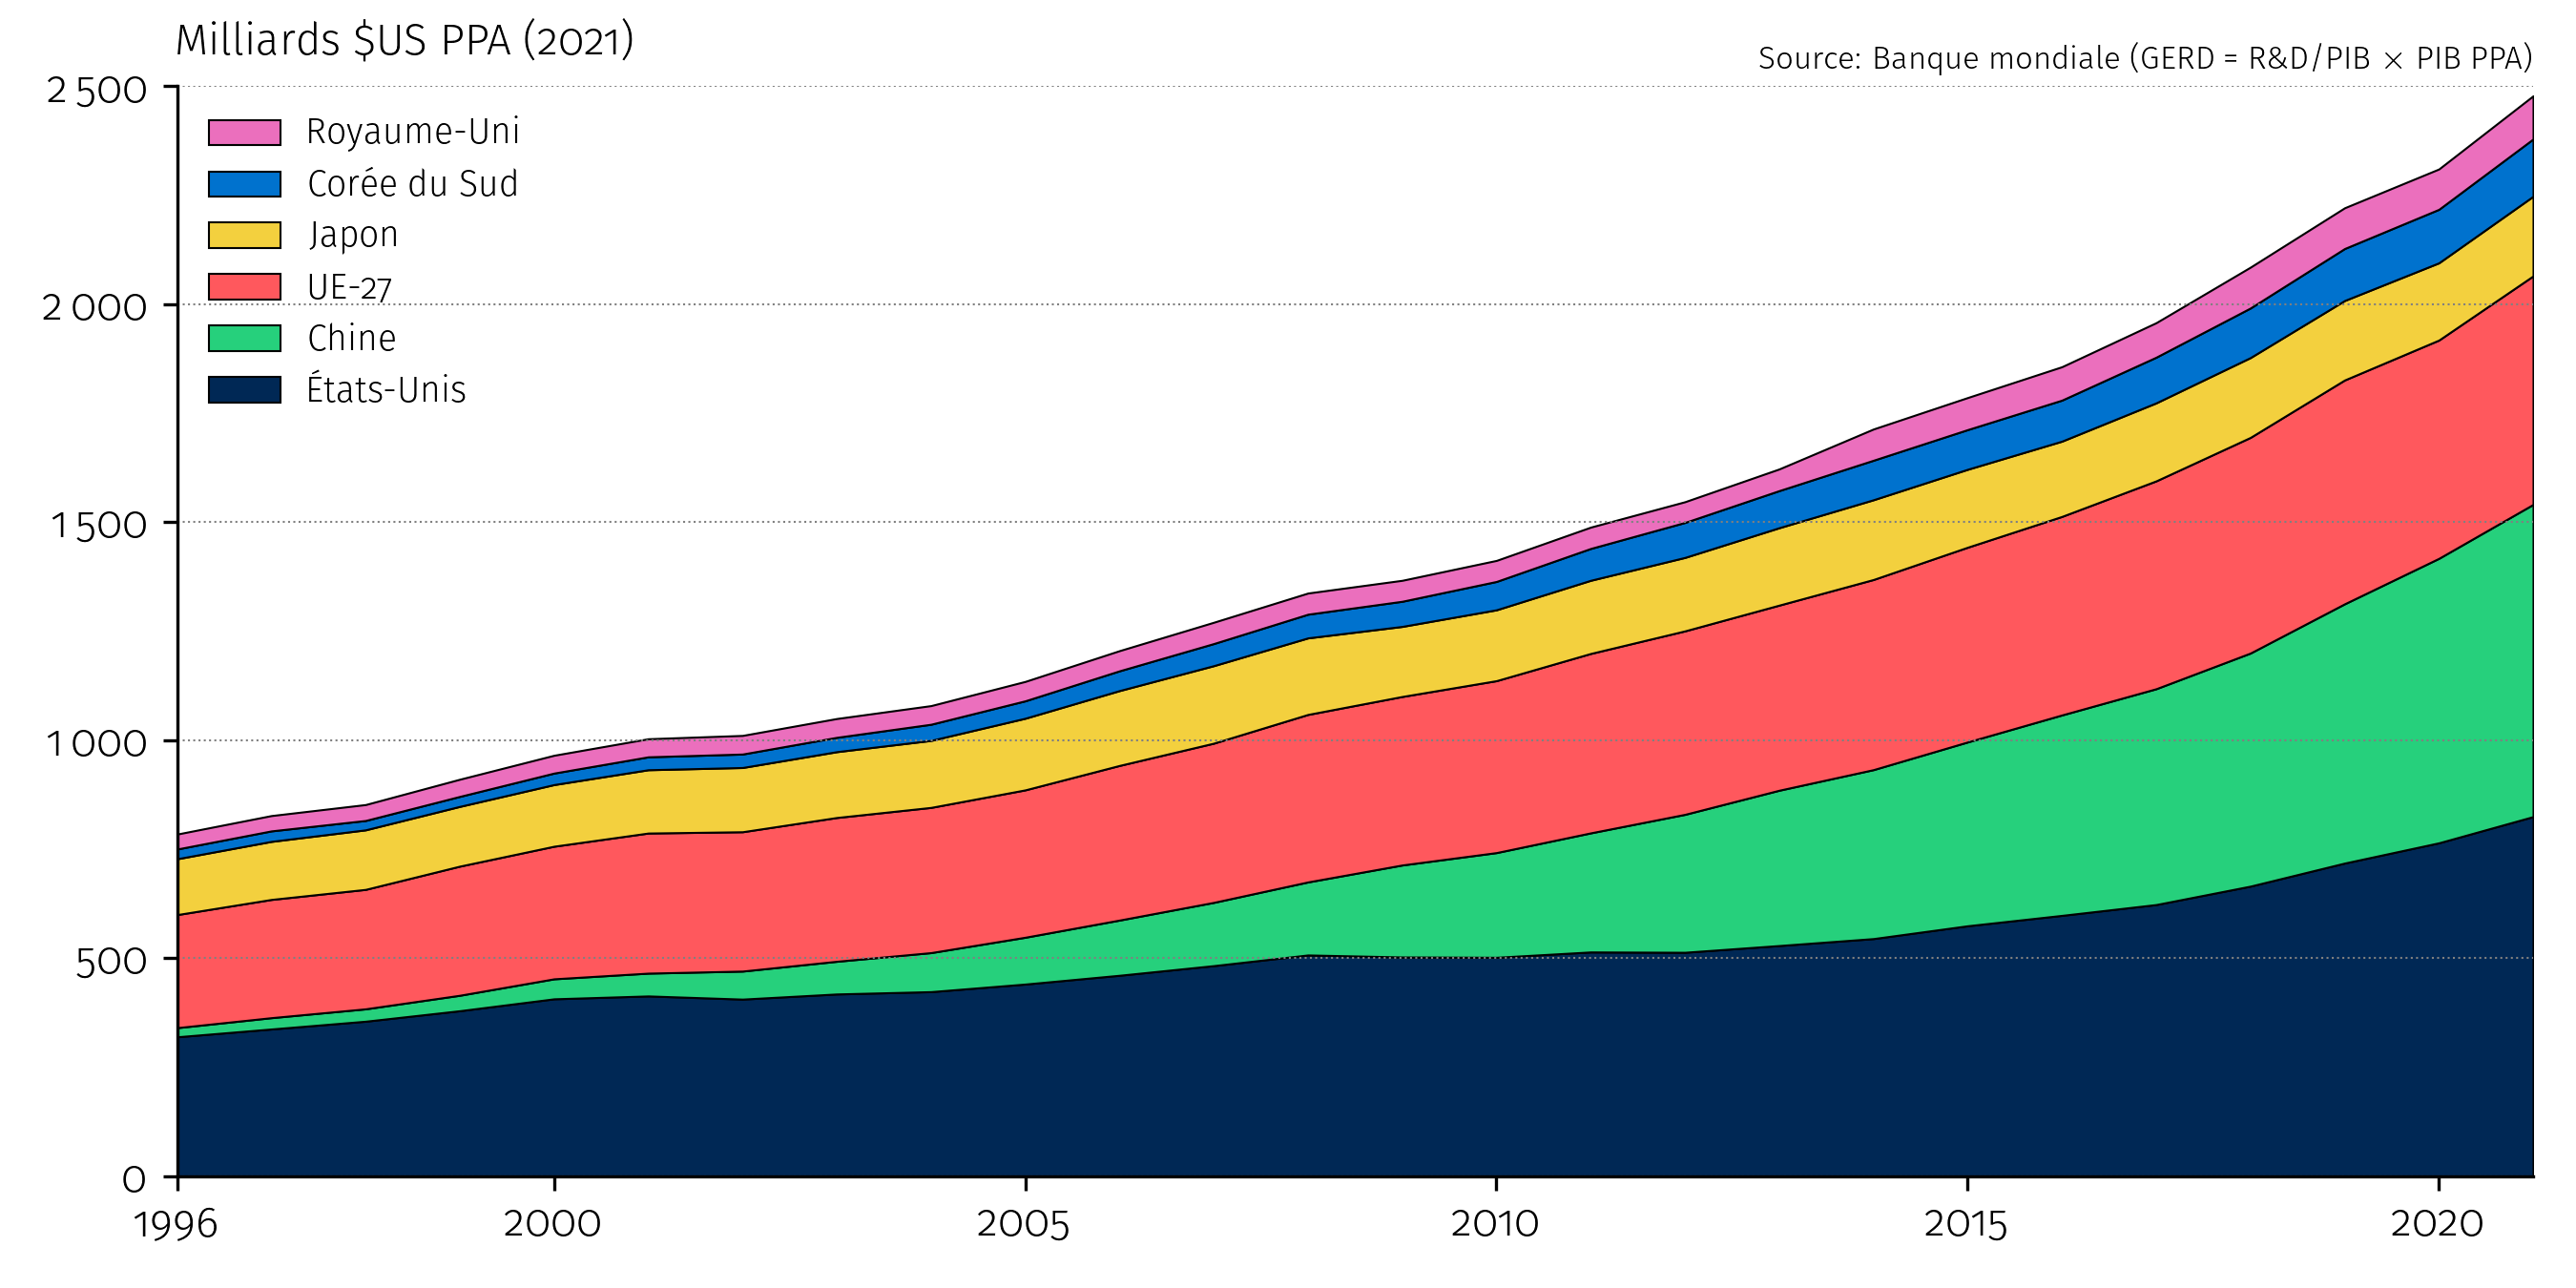
\includegraphics[width=0.95\textwidth]{rd_spending_global.png}
   \end{figure}
\end{frame}

\begin{frame}{La loi de Moore : un progrès exponentiel}
   \begin{figure}
      \centering
      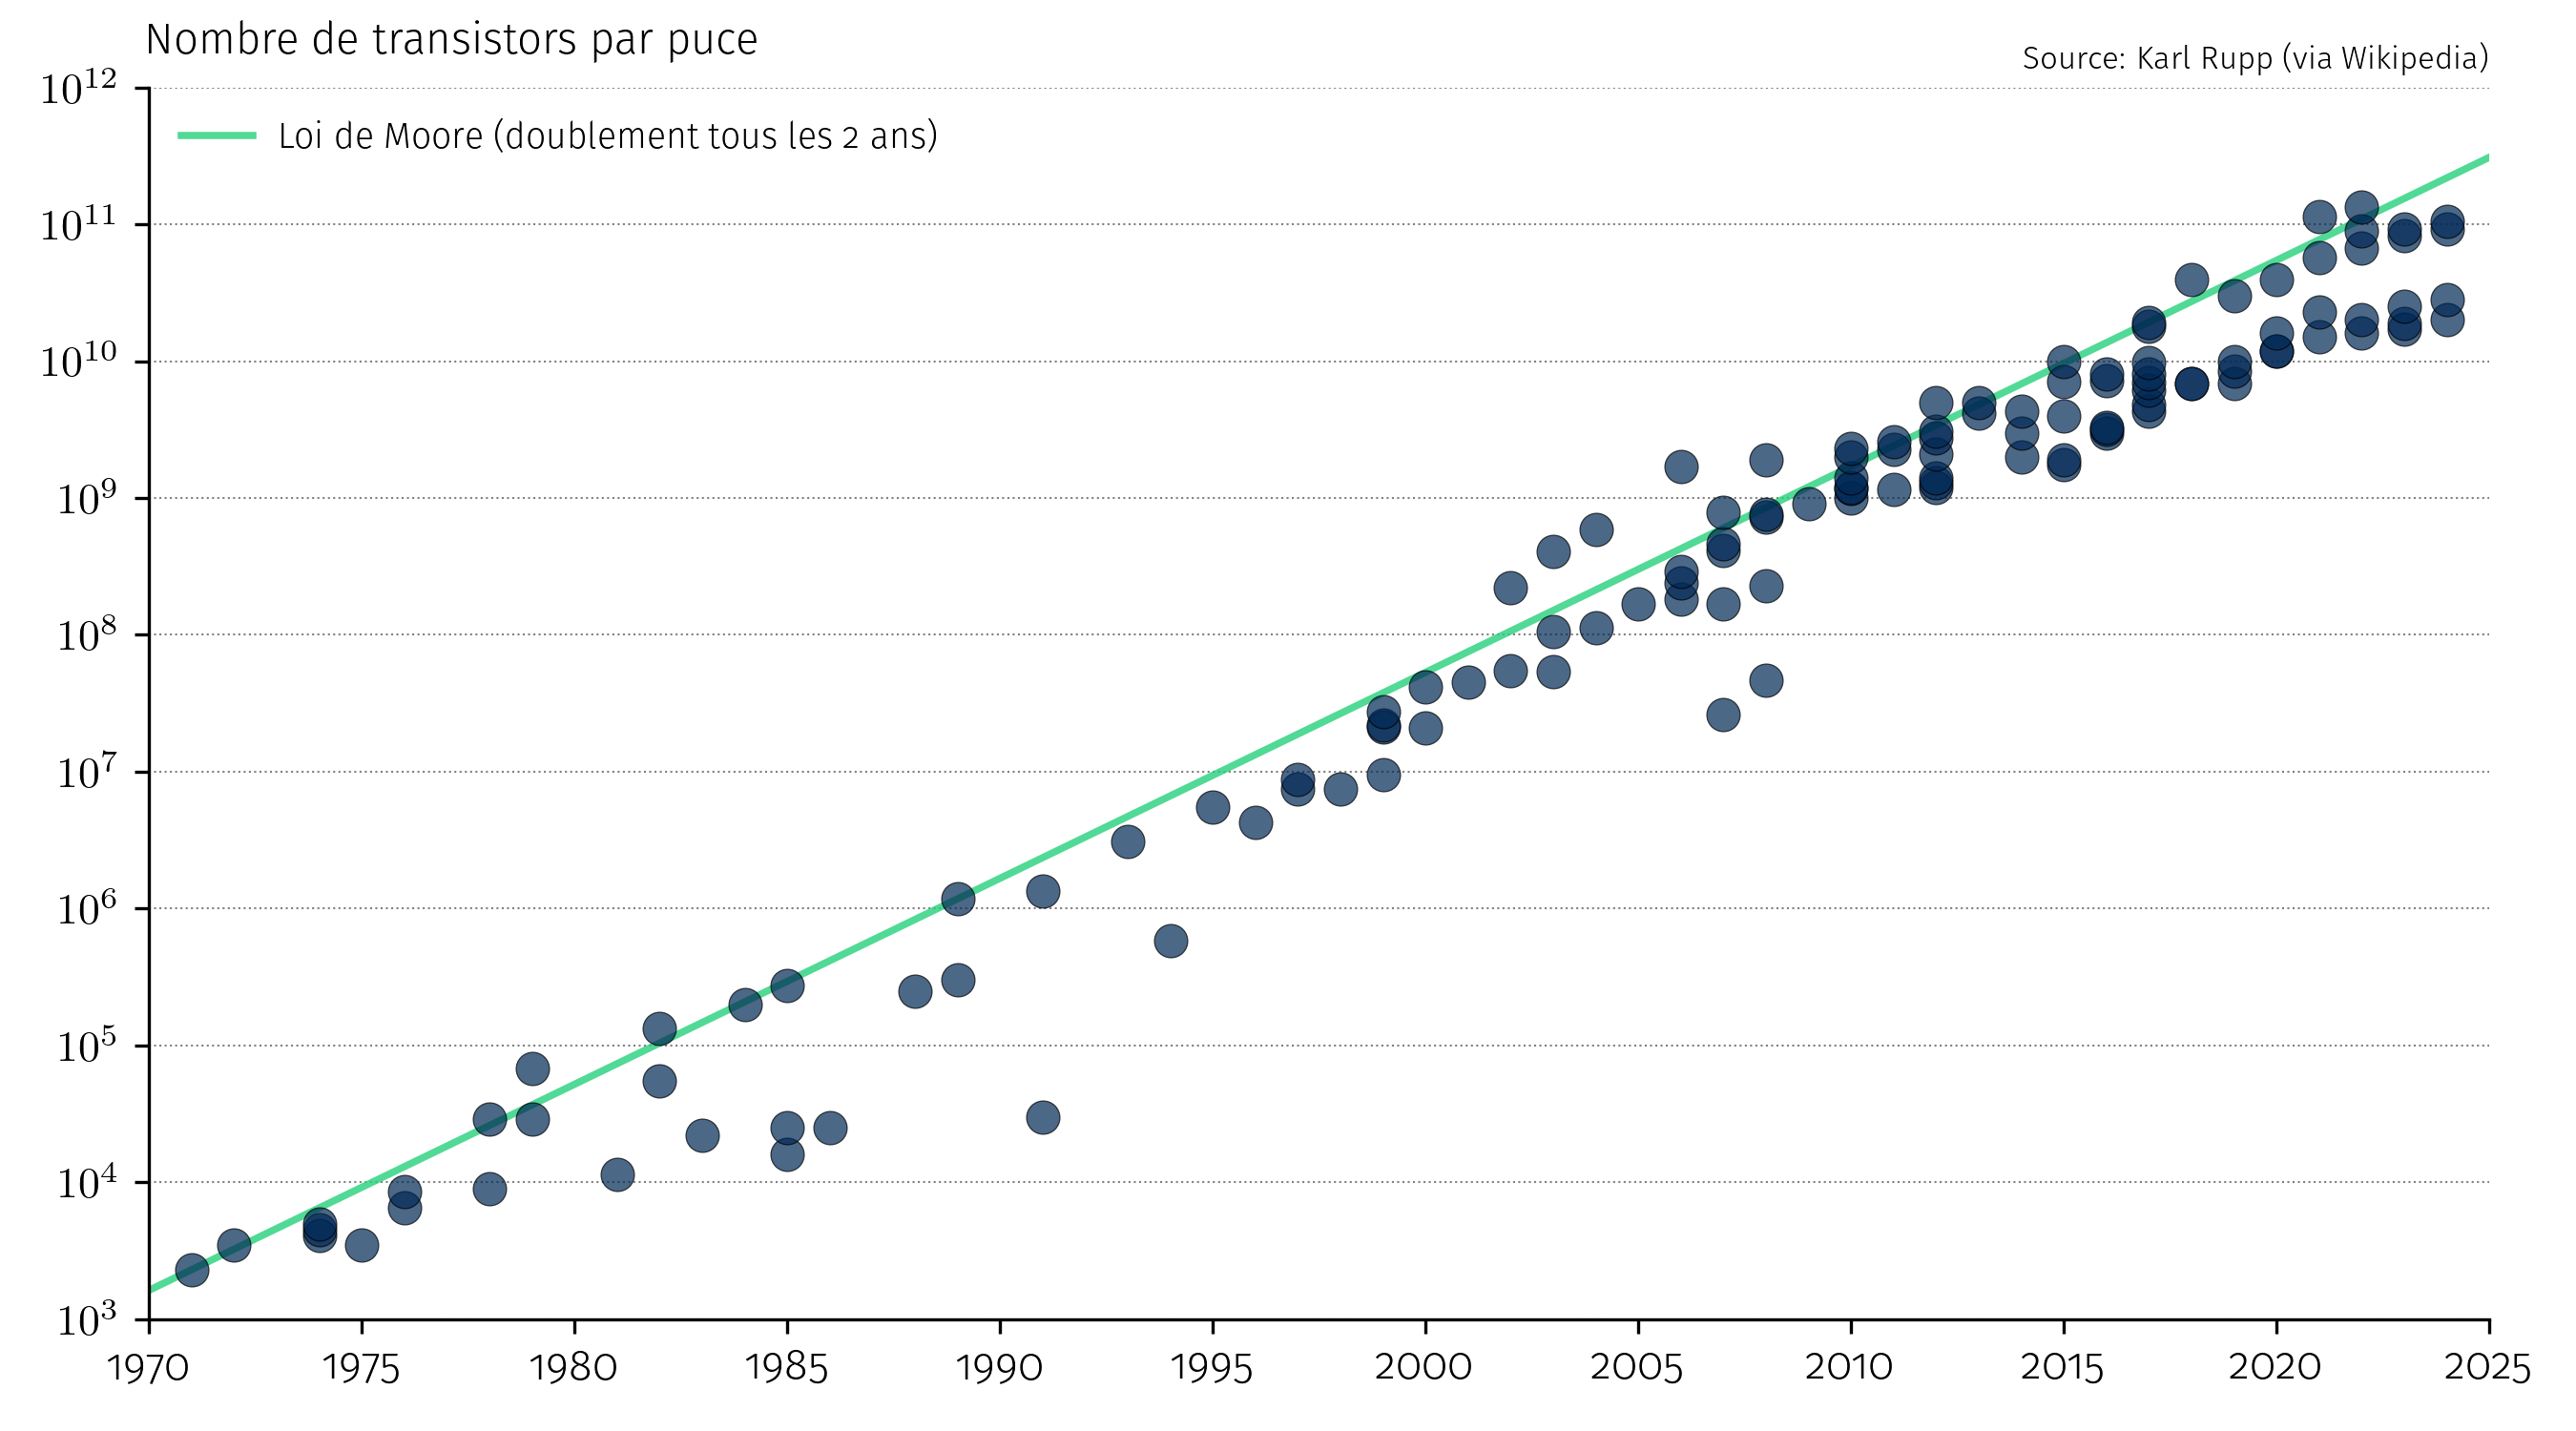
\includegraphics[width=0.95\textwidth]{moores_law.png}
   \end{figure}
\end{frame}

\begin{frame}[t]{Trois types de progrès technologique}
   \vspace{0.2cm}
   \begin{enumerate}
      \setlength\itemsep{0.4cm}
      \item \textbf{Innovation de produit} --- Créer quelque chose de nouveau
      \vspace{0.15cm}
      \begin{itemize}
         \setlength\itemsep{0.15cm}
         \item iPhone, vaccin ARNm, ChatGPT
         \item Retombées technologiques élevées (rétro-ingénierie)
      \end{itemize}
      \item \textbf{Innovation de procédé} --- Produire mieux ou moins cher
      \vspace{0.15cm}
      \begin{itemize}
         \setlength\itemsep{0.15cm}
         \item Chaîne de montage (Ford), conteneurisation, loi de Moore
         \item Retombées technologiques faibles (secret industriel)
      \end{itemize}
      \item \textbf{Adoption et diffusion} --- Déployer ce qui existe déjà
      \vspace{0.15cm}
      \begin{itemize}
         \setlength\itemsep{0.15cm}
         \item Électrification des usines (40 ans!), Solow paradox
         \item La plupart des pays croissent en adoptant, pas en inventant
      \end{itemize}
   \end{enumerate}
\end{frame}

\begin{frame}{La diffusion des technologies}
   \begin{figure}
      \centering
      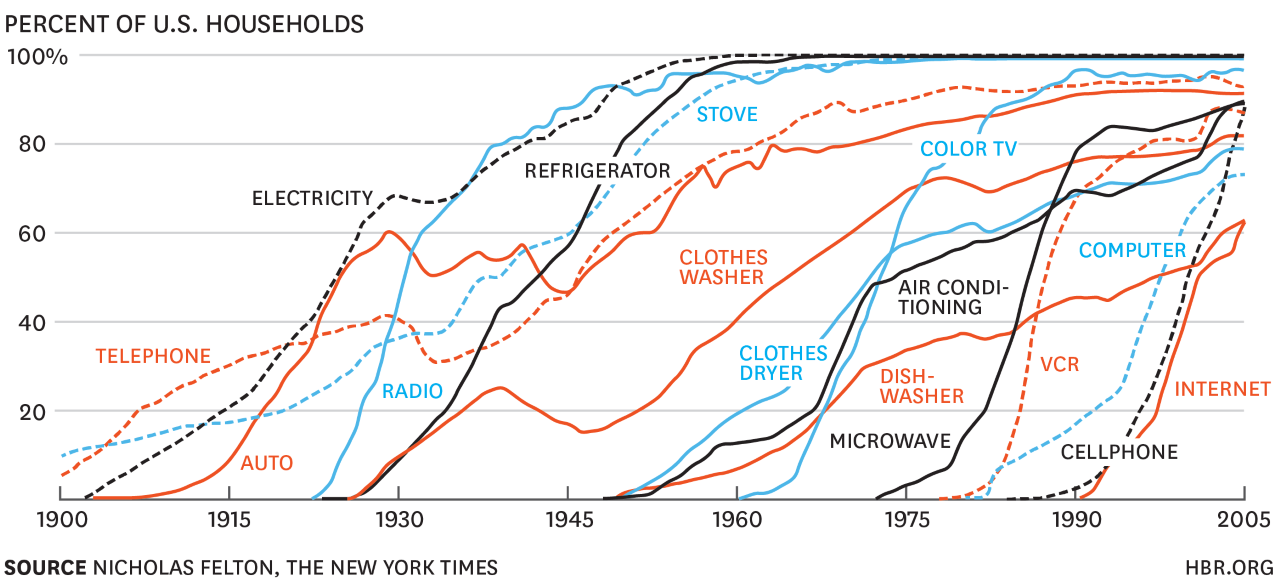
\includegraphics[width=0.95\textwidth, keepaspectratio]{technology_adoption_1.png}
   \end{figure}
\end{frame}

\begin{frame}{Les technologies se diffusent plus rapidement que par le passé}
   \begin{figure}
      \centering
      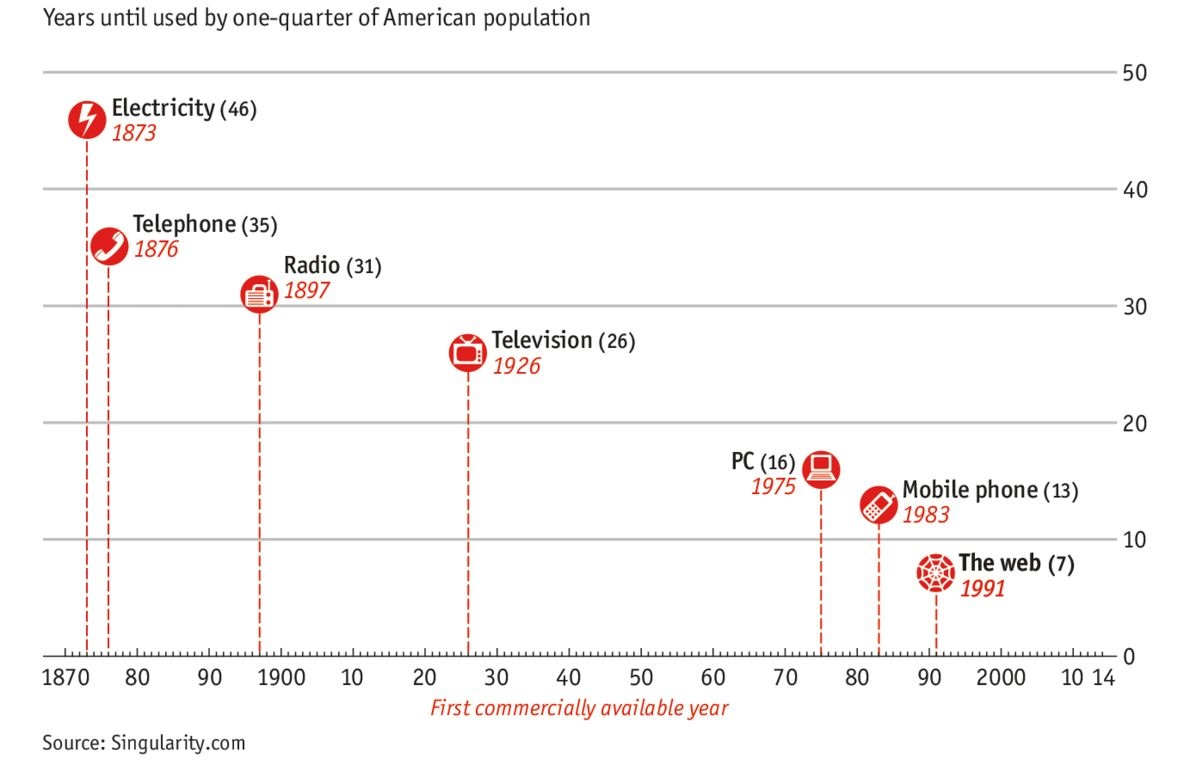
\includegraphics[height=0.8\textheight, keepaspectratio]{technology_adoption_2.jpeg}
   \end{figure}
\end{frame}

\begin{frame}{Pourquoi si peu de diffusion technologique?}
   \begin{figure}
      \centering
      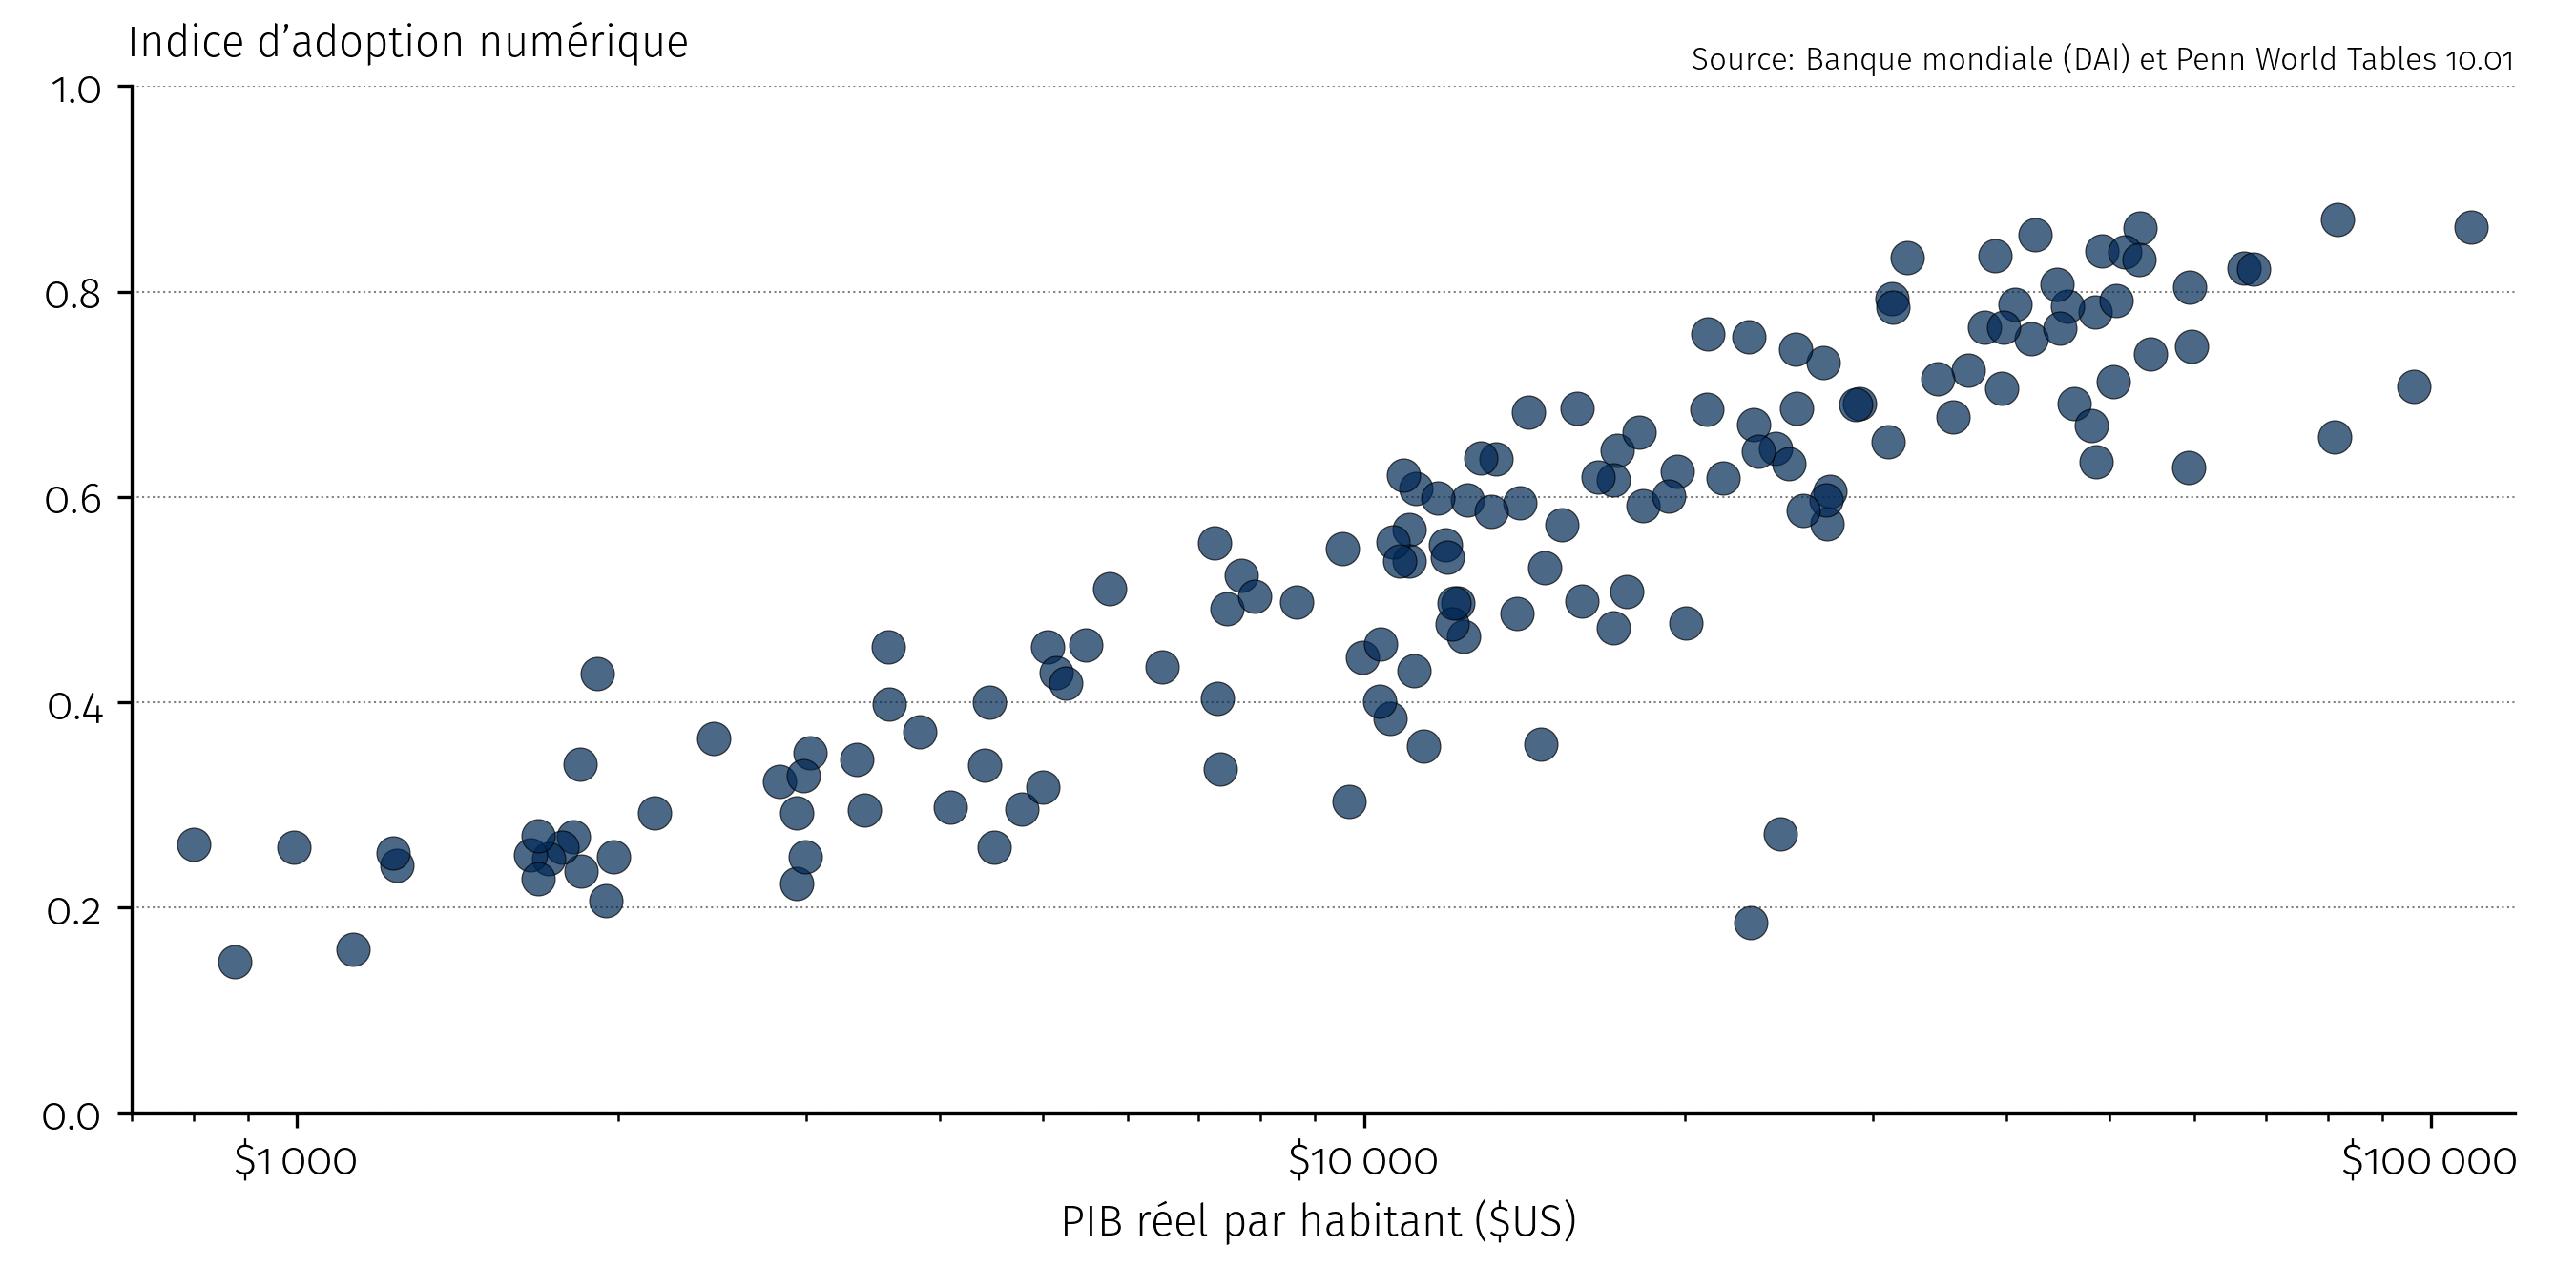
\includegraphics[width=0.95\textwidth, keepaspectratio]{dai.png}
   \end{figure}
\end{frame}

% --- 2. Géographie, climat, et culture ------------------------------------------------------

\begin{frame}{Théories de la PTF}
   \begin{enumerate}
      \setlength\itemsep{0.5cm}
      \item {\color{gray!50}Technologie et idées}
      \item \textbf{Géographie, climat, et culture}
      \item Capital humain
      \item Institutions
   \end{enumerate}
\end{frame}

\begin{frame}{La plupart des pays pauvres sont dans les tropiques}
   \begin{figure}
      \centering
      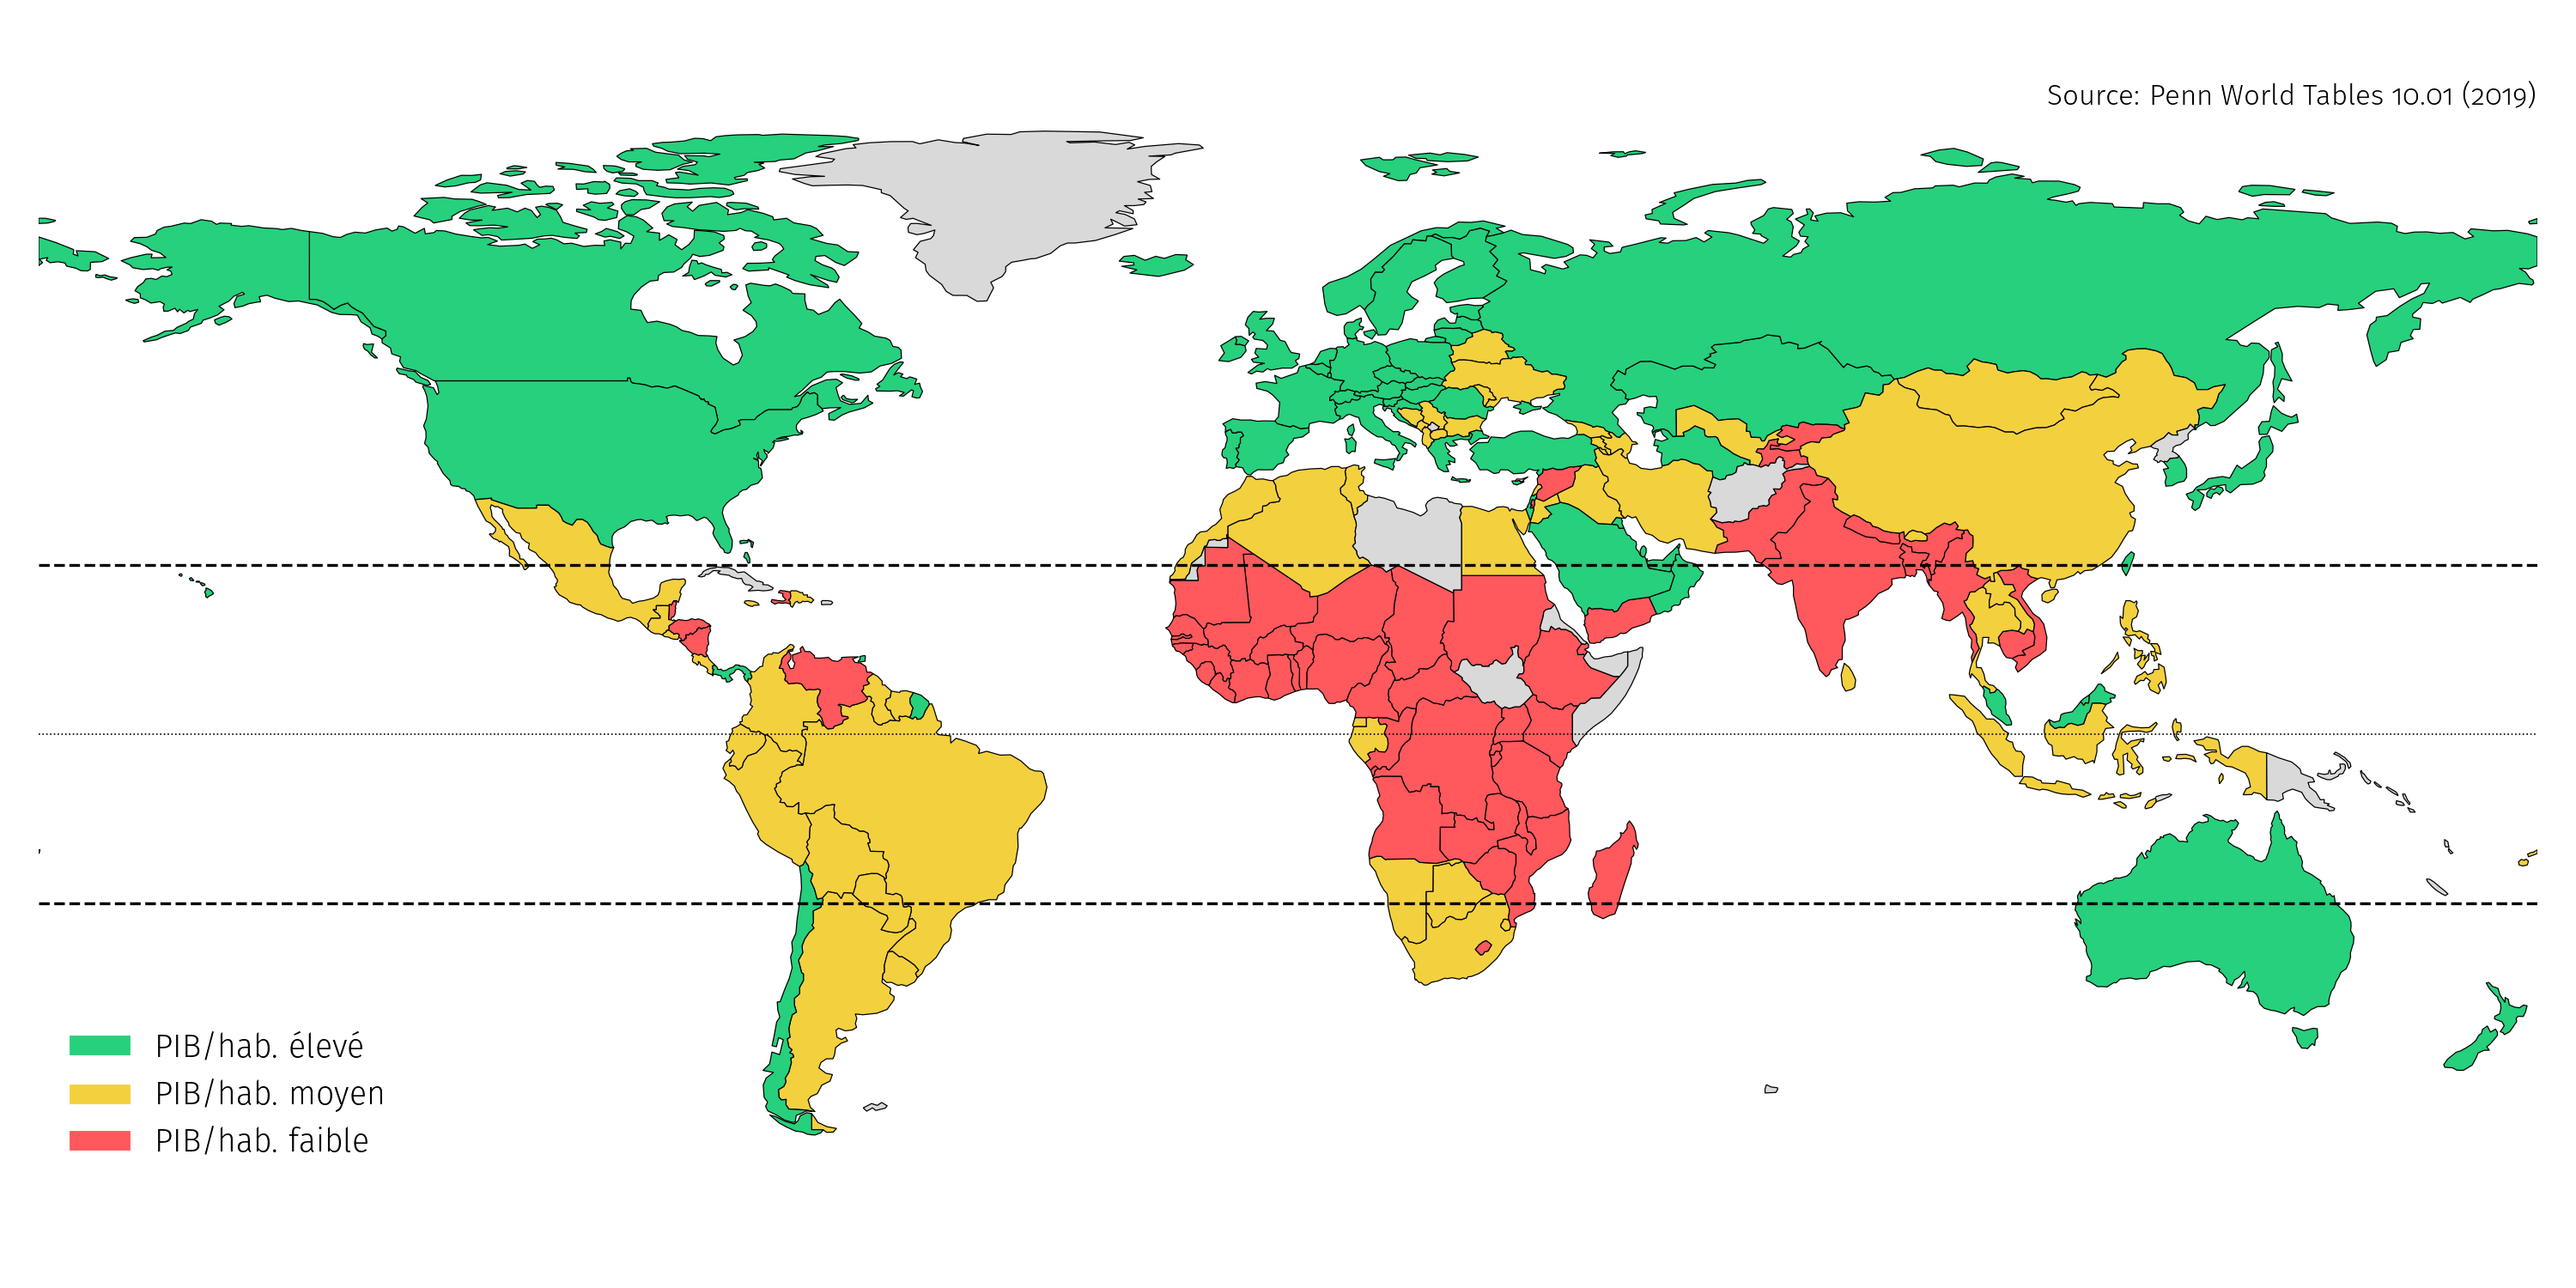
\includegraphics[width=0.95\textwidth, keepaspectratio]{tropics.png}
   \end{figure}
\end{frame}

\begin{frame}[t]{Géographie, climat, et culture}
   \small
   \textbf{Pourquoi les pays chauds sont-ils plus pauvres?}
   \vspace{0.1cm}
   \begin{itemize}
      \setlength\itemsep{0.1cm}
      \item Rendements agricoles plus faibles à haute température
      \item Maladies endémiques (malaria, parasites tropicaux)
   \end{itemize}
   \vspace{0.2cm}
   \textbf{Autres facteurs?}
   \vspace{0.1cm}
   \begin{itemize}
      \setlength\itemsep{0.1cm}
      \item Ressources naturelles (maladie hollandaise)
      \item Pays enclavés (sans accès à la mer)
      \item Culture, religion, valeurs
   \end{itemize}
   \vspace{0.1cm}
   \begin{warning}[Limites de ces explications]
      Le secteur primaire ne représente qu'une faible part du PIB dans les pays riches\ldots
   \end{warning}
\end{frame}

\begin{frame}[t]{Mais comment expliquer ces différences?}
   \vfill
   \begin{columns}[T,onlytextwidth]
      \column{0.33\textwidth}
         \centering
         \textbf{{\footnotesize Corée du Nord vs. Sud}}\\[0.5ex]
         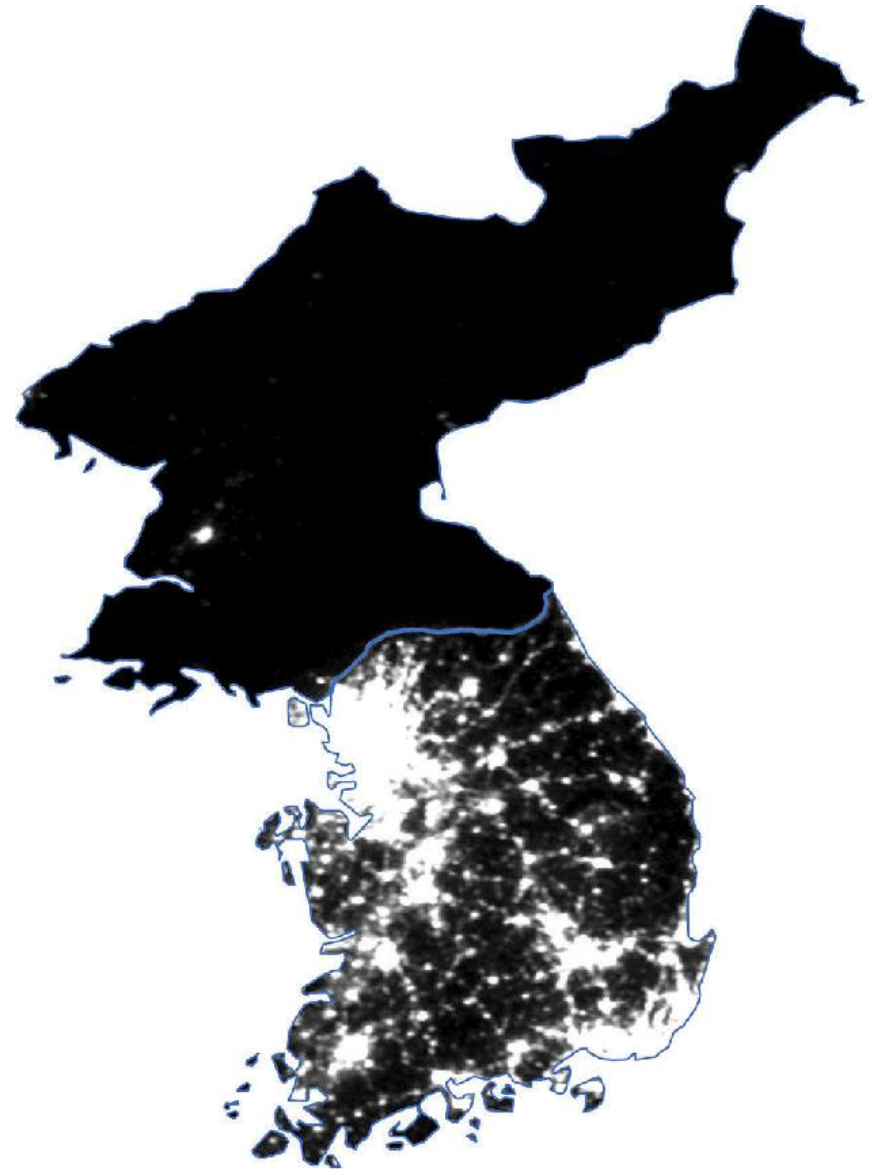
\includegraphics[width=\linewidth, height=0.5\textheight, keepaspectratio]{korea_satellite.png}
      \column{0.33\textwidth}
         \centering
         \textbf{{\footnotesize Allemagne Ouest vs. Est}}\\[0.5ex]
         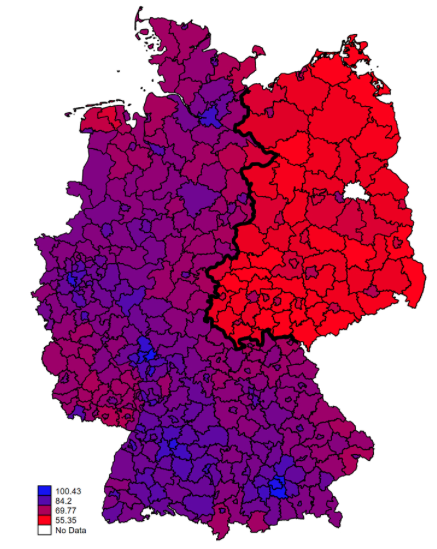
\includegraphics[width=\linewidth, height=0.5\textheight, keepaspectratio]{germany_wage.png}
      \column{0.33\textwidth}
         \centering
         \textbf{{\footnotesize Amérique du Nord vs. Sud}}\\[0.5ex]
         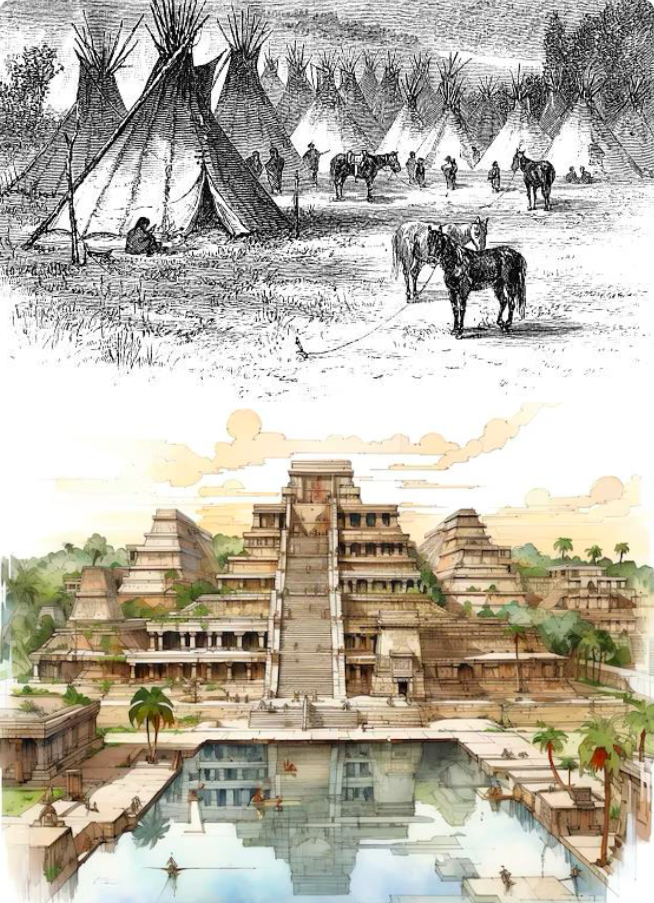
\includegraphics[width=\linewidth, height=0.5\textheight, keepaspectratio]{fortune_reversal.png}
   \end{columns}
   \vfill
\end{frame}

\begin{frame}{Zimbabwe vs.\ Botswana}
   \begin{figure}
      \centering
      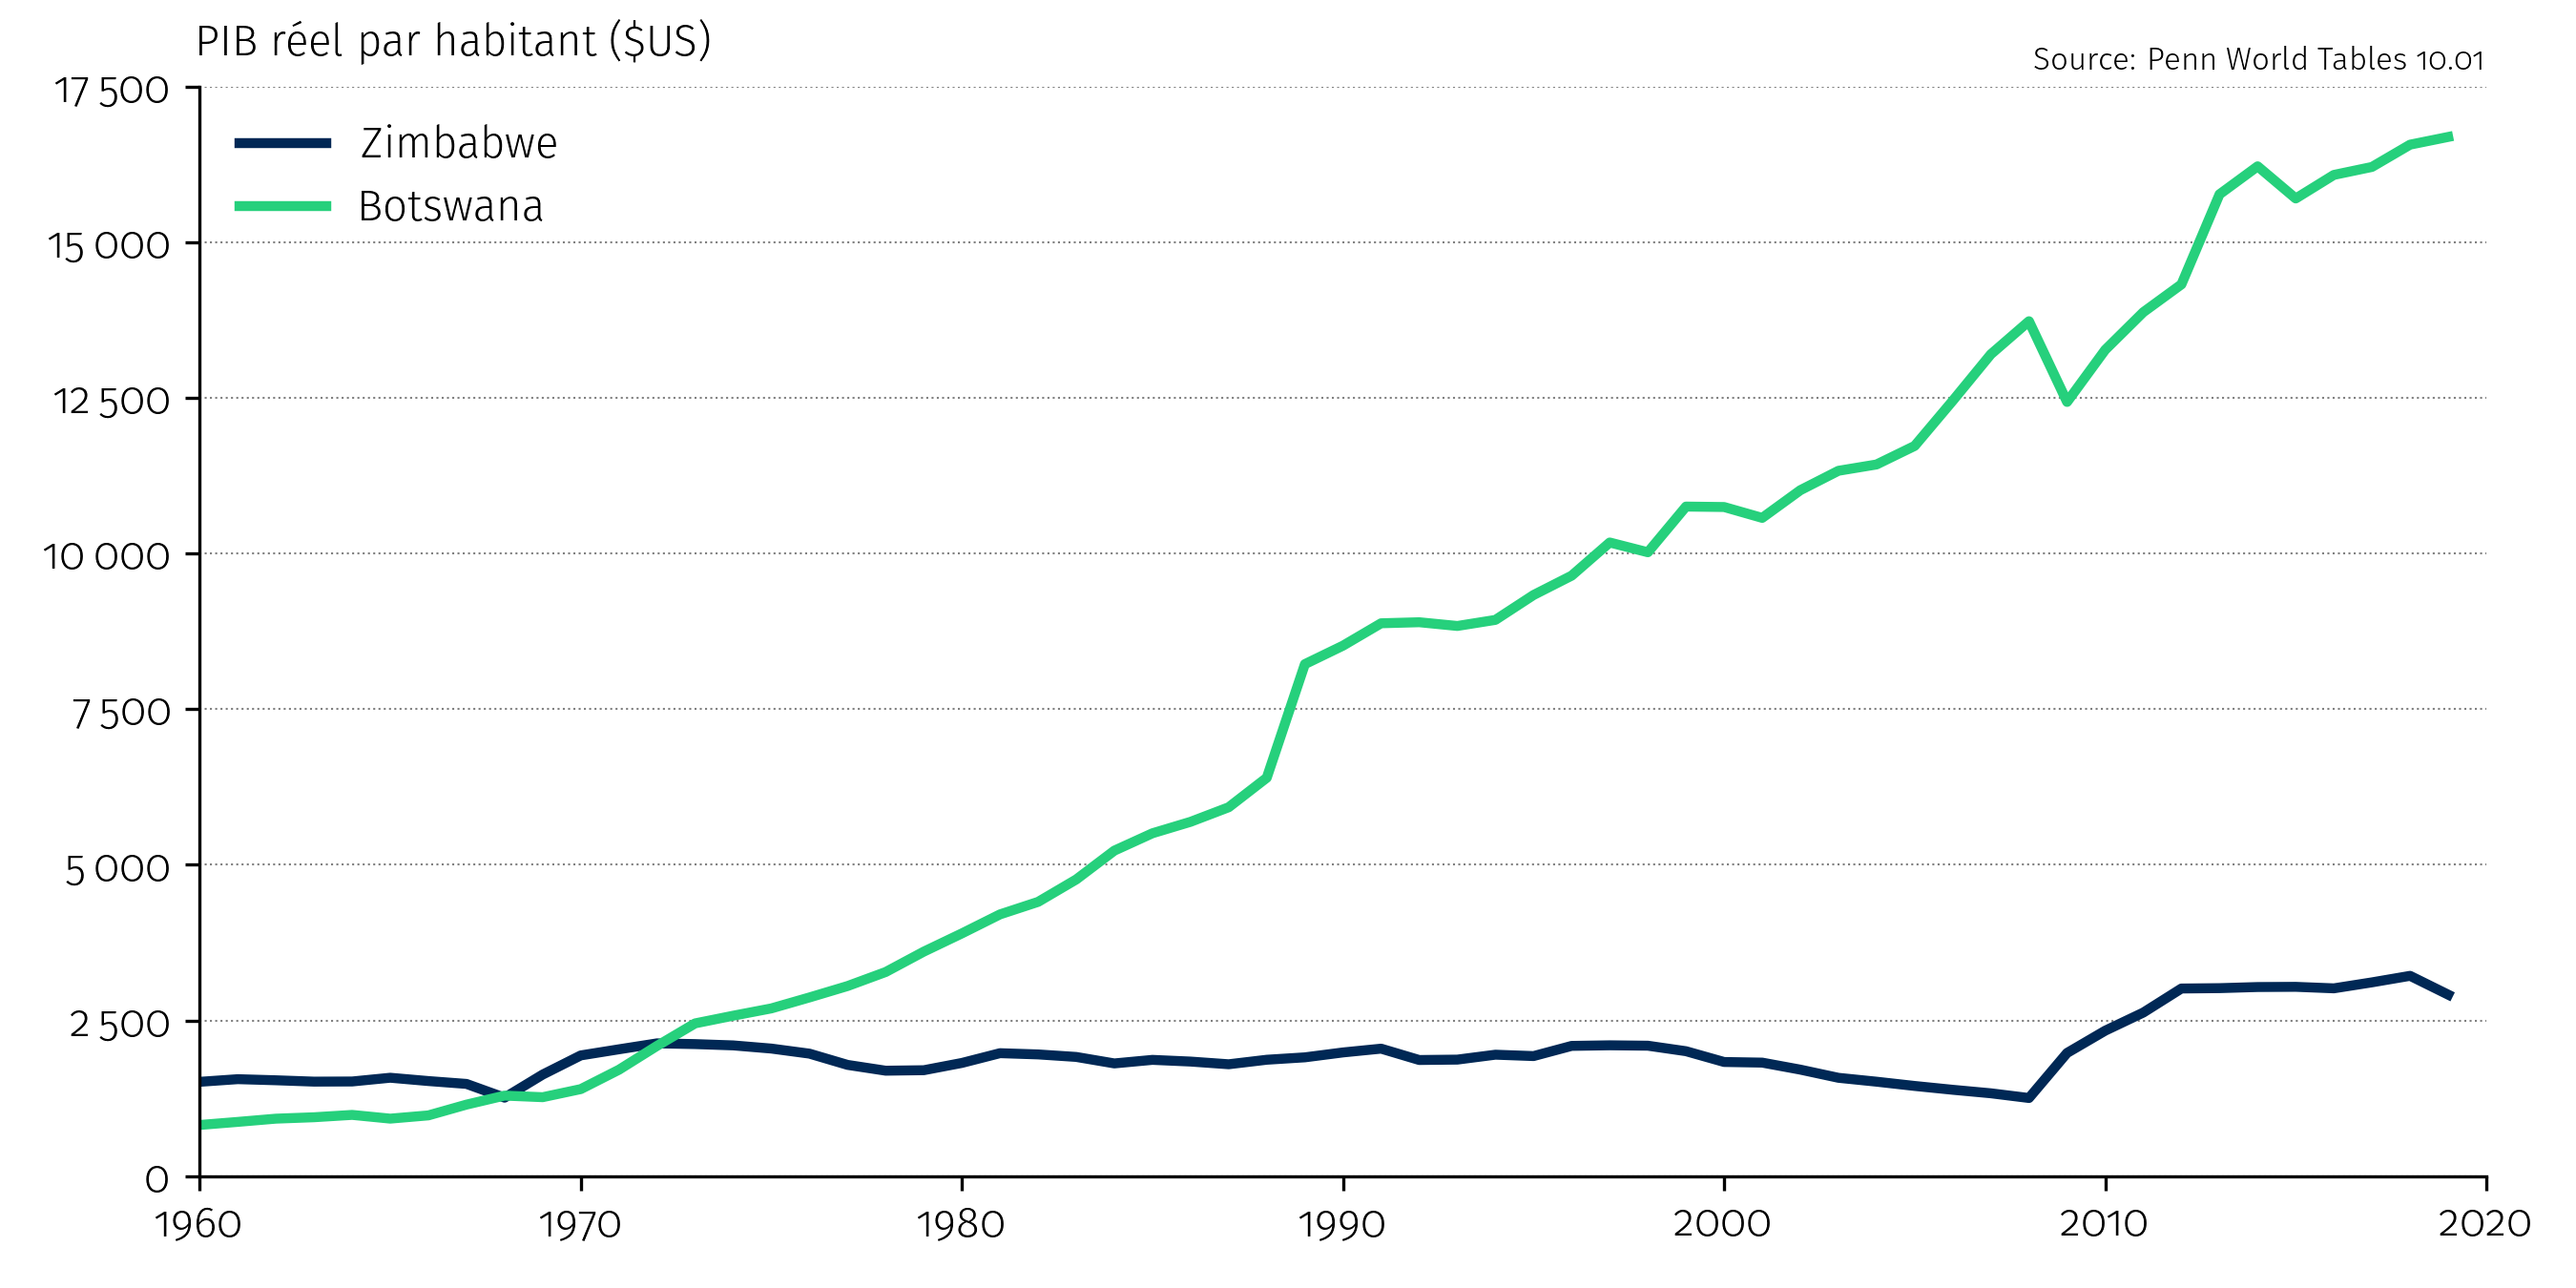
\includegraphics[width=0.95\textwidth]{zimbabwe_botswana.png}
   \end{figure}
\end{frame}

\begin{frame}{Théories de la PTF}
   \begin{enumerate}
      \setlength\itemsep{0.5cm}
      \item {\color{gray!50}Technologie et idées}
      \item {\color{gray!50}Géographie, climat, et culture}
      \item \textbf{Capital humain}
      \item Institutions
   \end{enumerate}
\end{frame}

% --- 3. Capital humain ------------------------------------------------------

\begin{frame}{Éducation $\to$ prospérité?}
   \begin{figure}
      \centering
      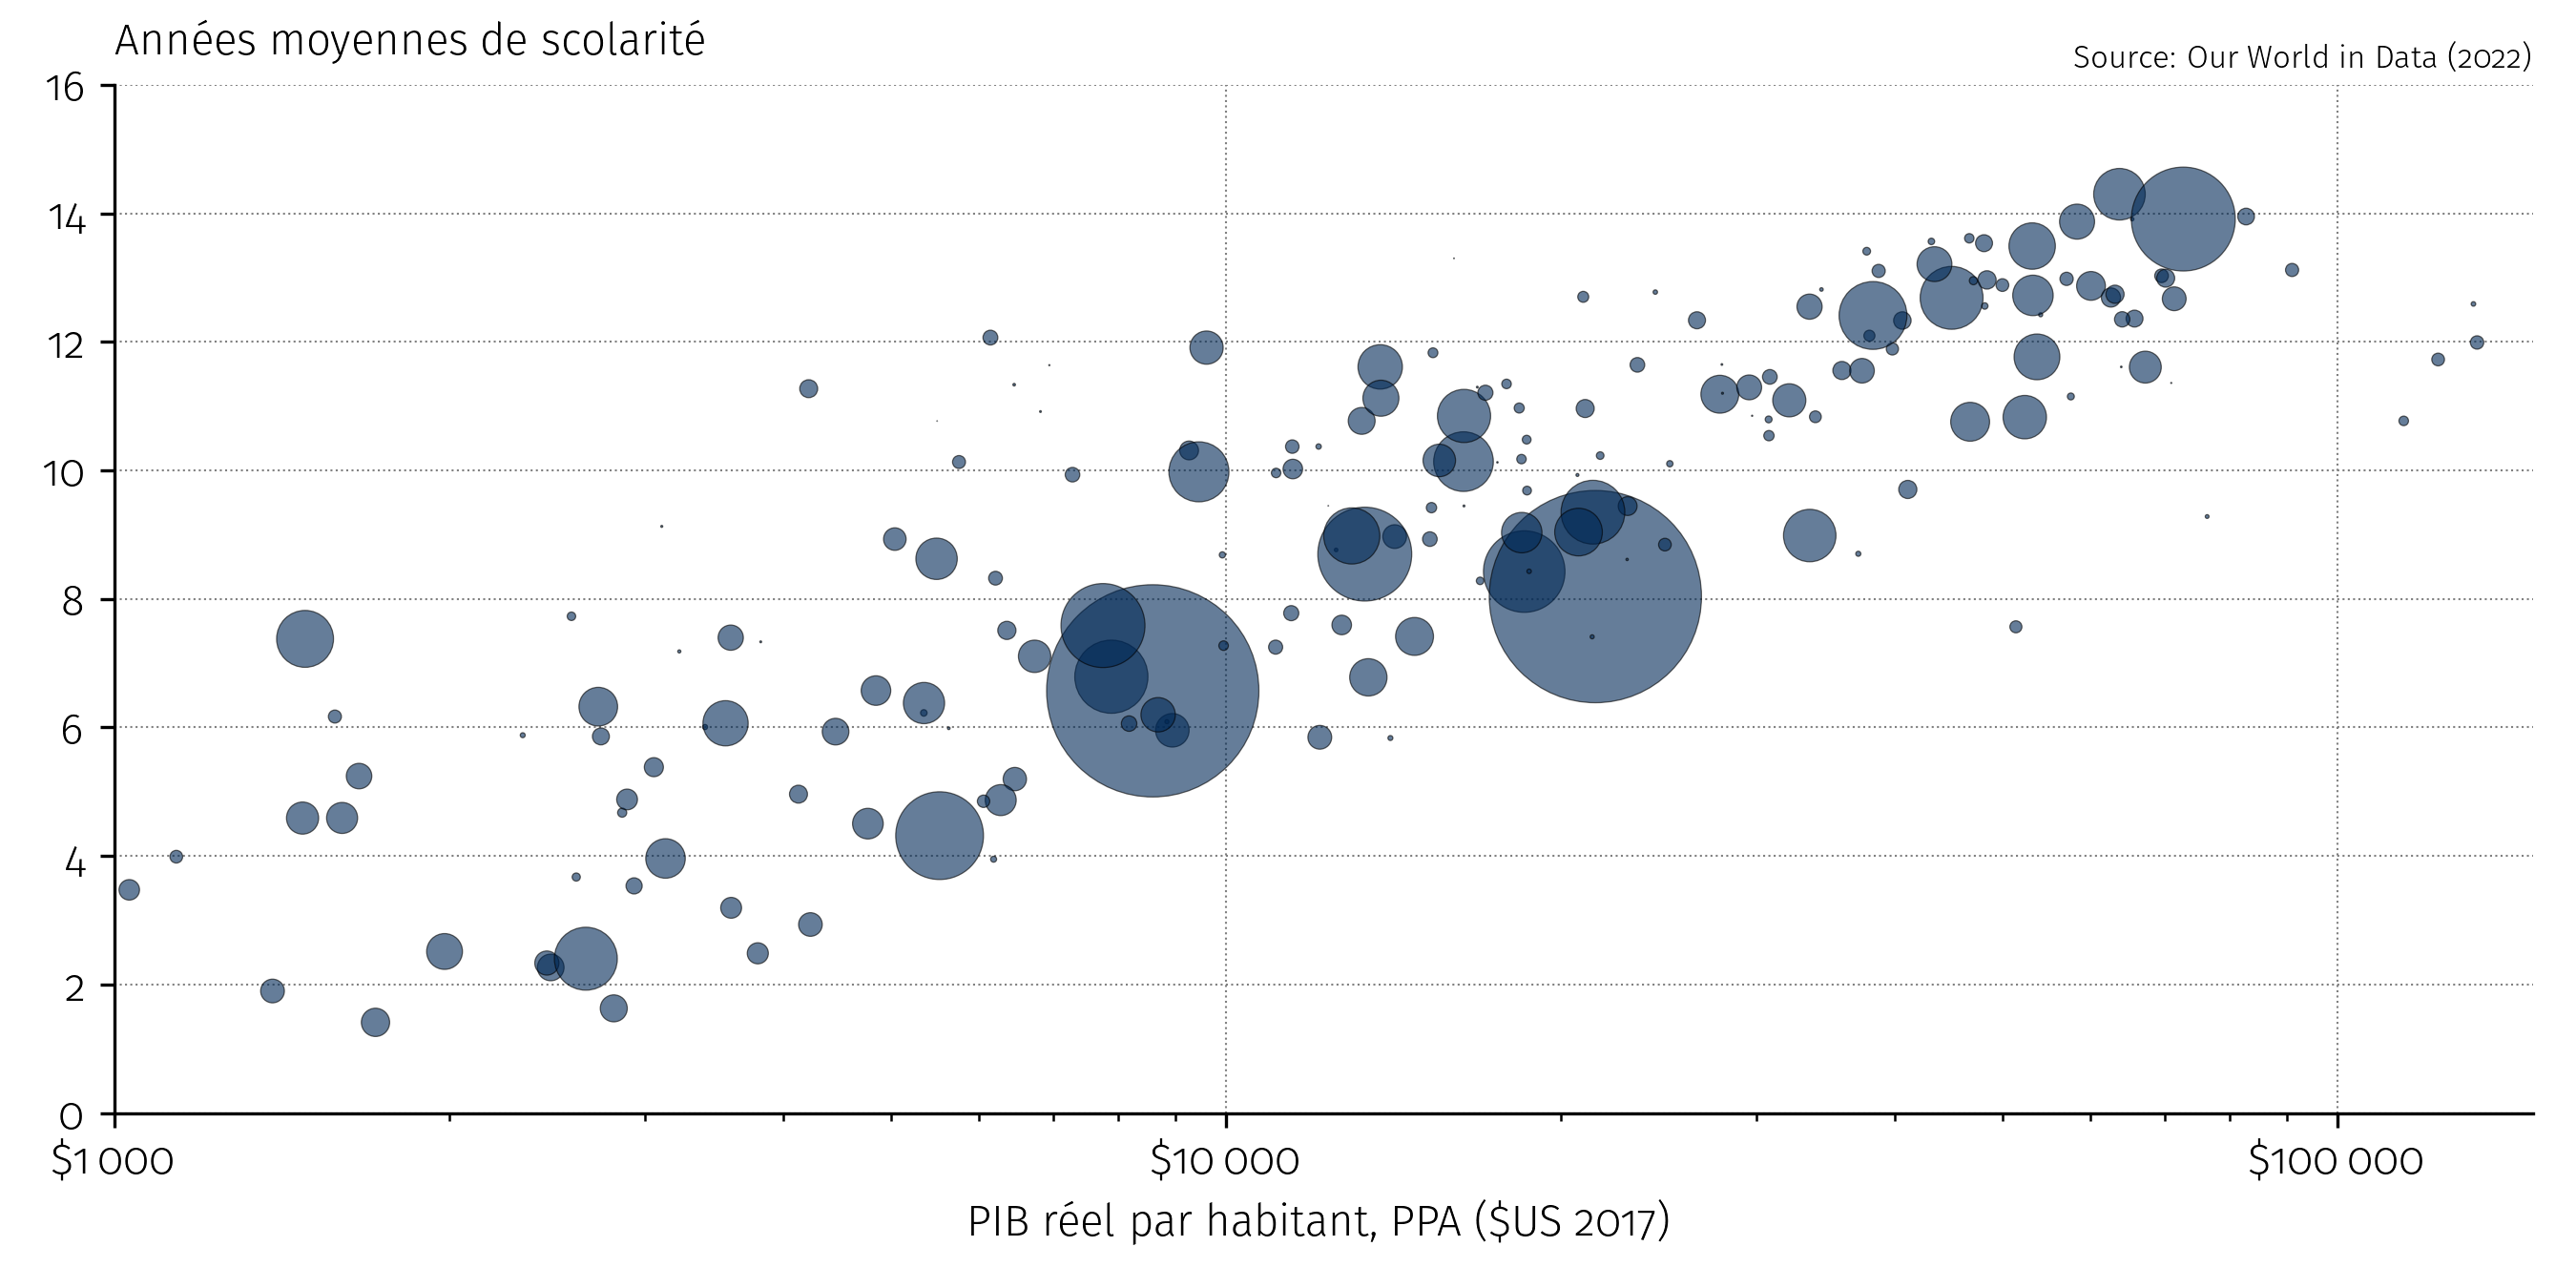
\includegraphics[width=0.95\textwidth, keepaspectratio]{schooling.png}
   \end{figure}
\end{frame}

\begin{frame}[t]{Qu'est-ce que le capital humain?}
   \small
   \textbf{Productivité incarnée dans les connaissances, compétences et talents des individus.}
   \vspace{0.2cm}
   \begin{itemize}
      \setlength\itemsep{0.15cm}
      \item Accumulé par l'\textbf{éducation} et la \textbf{formation}
      \item Preuve empirique : des travailleurs différents reçoivent des salaires très différents
      \item Augmenter le capital humain ($H$) $\to$ augmenter la PTF \textbf{effective}
   \end{itemize}
   \vspace{0.15cm}
   \begin{warning}[Corrélation $\neq$ causalité]
      Les pays riches ont plus de capital humain, mais la causalité peut être \textbf{inversée} : la richesse permet d'investir davantage en éducation. \\

      Le lien causal éducation $\to$ prospérité n'explique qu'un tiers de la corrélation\ldots\\
      \mbox{}\hfill{\scriptsize\textcolor{HECgray}{Bils \& Klenow, \textit{AER}, 2000}}
   \end{warning}
\end{frame}

\begin{frame}{Le capital humain a très peu de pouvoir explicatif\ldots}
   \begin{figure}
      \centering
      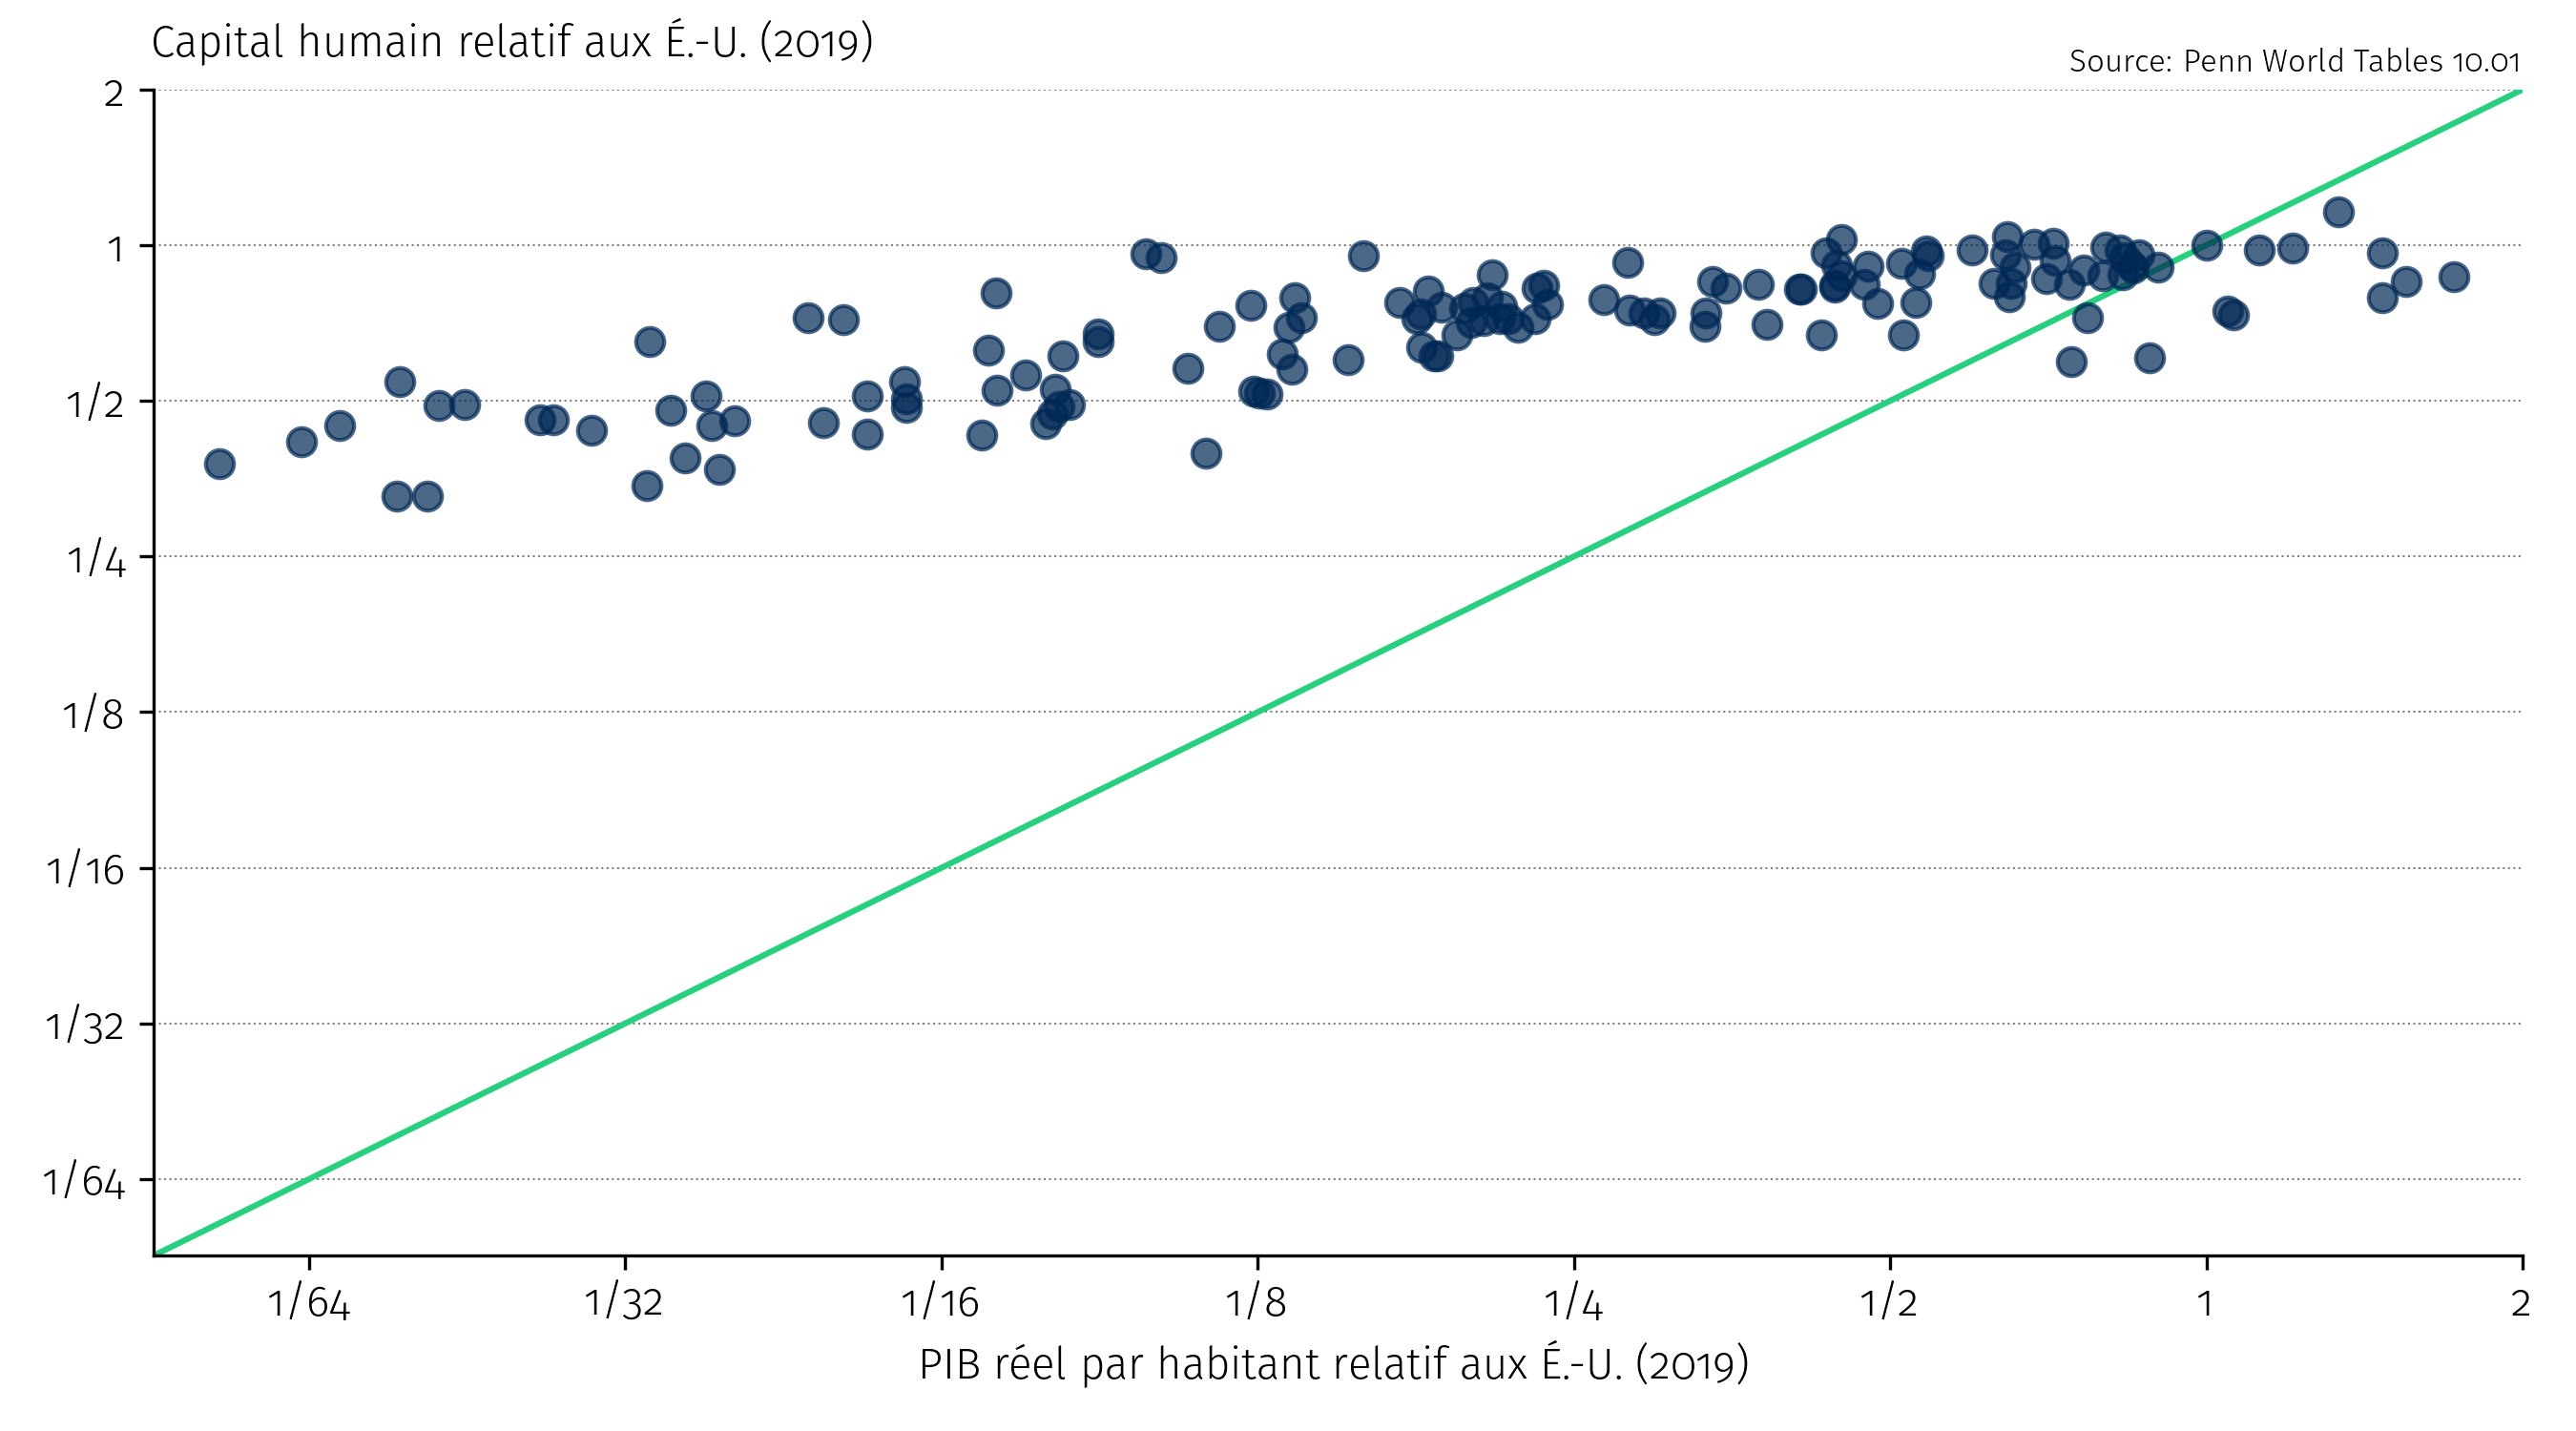
\includegraphics[width=0.95\textwidth]{development_accounting_human_capital.png}
   \end{figure}
\end{frame}

% --- 4. Institutions ---------------------------------------------------------

\begin{frame}{Théories de la PTF}
   \begin{enumerate}
      \setlength\itemsep{0.5cm}
      \item {\color{gray!50}Technologie et idées}
      \item {\color{gray!50}Géographie, climat, et culture}
      \item {\color{gray!50}Capital humain}
      \item \textbf{Institutions}
   \end{enumerate}
\end{frame}

\begin{frame}[t]{Les institutions comme \guillemotleft~règles du jeu~\guillemotright}
   \small
   \textbf{Institutions politiques et juridiques :}
   \vspace{0.15cm}
   \begin{itemize}
      \setlength\itemsep{0.1cm}
      \item État de droit (droits de propriété)
      \item Idéologie (méritocratie)
      \item Bureaucratie (\guillemotleft~paperasserie~\guillemotright)
      \item Stabilité politique
      \item Corruption
   \end{itemize}
   \vspace{0.2cm}
   \begin{keyinsight}
      Les règles du jeu façonnent les \textbf{incitations} à participer aux activités productives.
   \end{keyinsight}
\end{frame}

\begin{frame}[t]{Acemoglu, Johnson \& Robinson (Prix Nobel 2024)}
   \vspace{-0.1cm}
   \begin{center}
      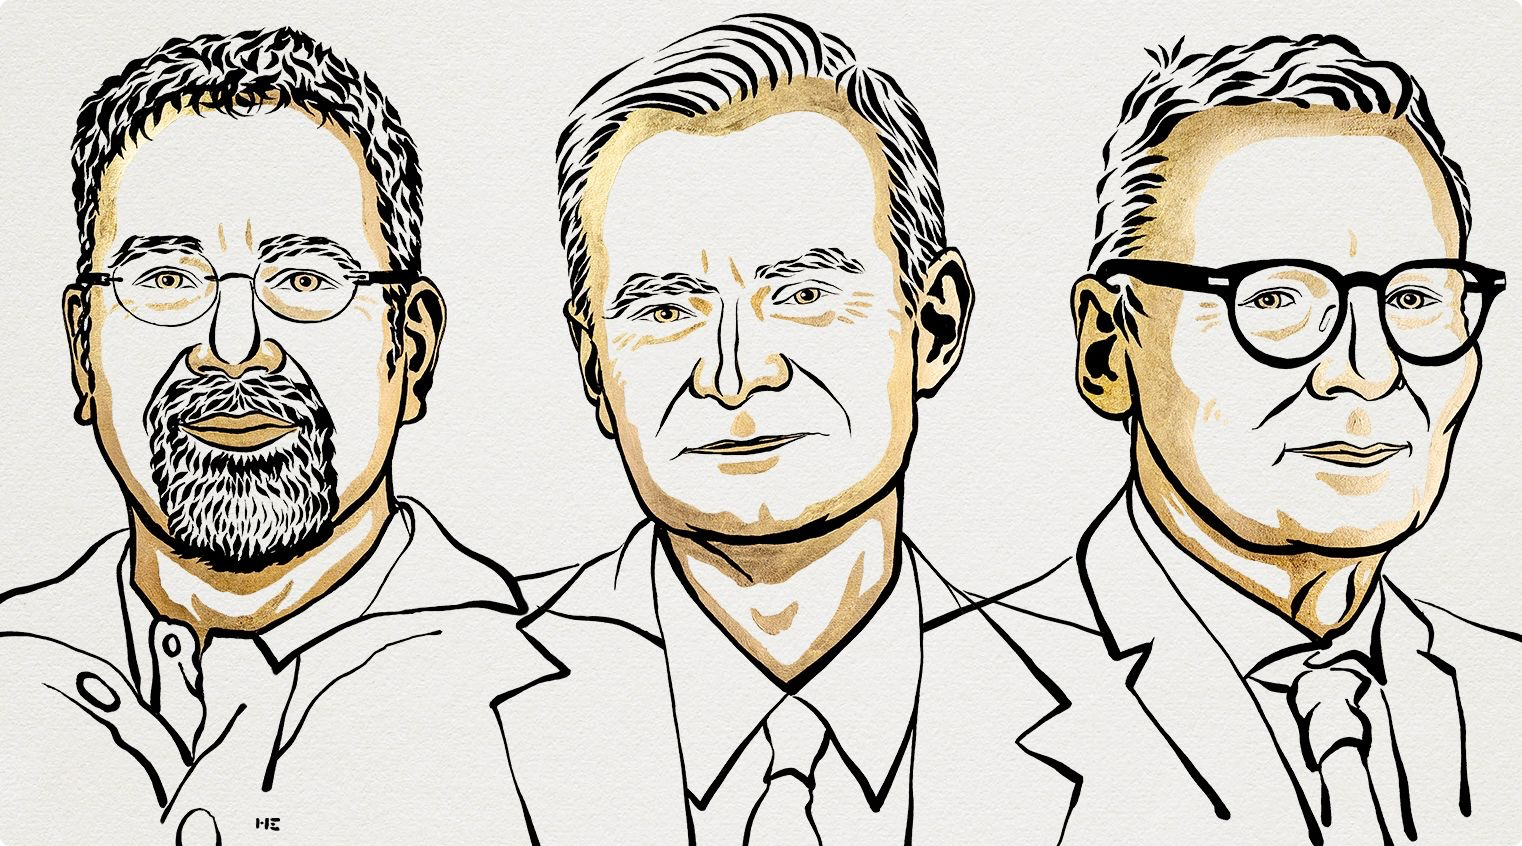
\includegraphics[height=5cm, keepaspectratio]{nobel_2024.png}%
      \hspace{0.4cm}%
      
\includegraphics[height=5cm, keepaspectratio]{why_nations_fail_book.png}
   \end{center}
   \begin{itemize}
      \small
      \setlength\itemsep{0.1cm}
      \item \textbf{Institutions inclusives :} état de droit $+$ concurrence $\to$ innovation
      \item \textbf{Institutions extractives :} corruption $+$ expropriation $\to$ stagnation
   \end{itemize}
\end{frame}

\begin{frame}[t]{Sommaire : théories de la productivité}
   \small
   \vspace{0.1cm}
   La croissance à l'échelle mondiale peut être caractérisée par\ldots
   \begin{columns}[T,onlytextwidth]
      \begin{column}{0.30\textwidth}
         \begin{tcolorbox}[colback=HECgreen!8, colframe=HECgreen, boxrule=0.5pt, arc=8pt,
            top=4pt, bottom=4pt, left=6pt, right=6pt]
            \centering\footnotesize\textbf{Économies matures}\\[3pt]
            En ralentissement\ldots
         \end{tcolorbox}
      \end{column}
      \begin{column}{0.30\textwidth}
         \begin{tcolorbox}[colback=HECnavy!8, colframe=HECnavy, boxrule=0.5pt, arc=8pt,
            top=4pt, bottom=4pt, left=6pt, right=6pt]
            \centering\footnotesize\textbf{Économies émergentes}\\[3pt]
            En rattrapage\ldots
         \end{tcolorbox}
      \end{column}
      \begin{column}{0.30\textwidth}
         \begin{tcolorbox}[colback=HECcoral!8, colframe=HECcoral, boxrule=0.5pt, arc=8pt,
            top=4pt, bottom=4pt, left=6pt, right=6pt]
            \centering\footnotesize\textbf{Économies stagnantes}\\[3pt]
            Peinent à décoller\ldots
         \end{tcolorbox}
      \end{column}
   \end{columns}
   \vspace{0.25cm}
   Le succès repose sur des \textbf{conditions appropriées} :
   \vspace{0.1cm}
   \begin{itemize}
      \setlength\itemsep{0.1cm}
      \item La prospérité coïncide rarement avec un contexte institutionnel faible
      \item Des institutions inclusives encouragent l'innovation et la productivité
   \end{itemize}
   \begin{bizimplication}
      \footnotesize Pour un gestionnaire, comprendre le cadre institutionnel d'une économie est aussi important que de comprendre ses fondamentaux macroéconomiques.
   \end{bizimplication}
\end{frame}

\begin{frame}[t]{La main d'{\oe}uvre comme source de croissance}
   \begin{figure}
      \centering
      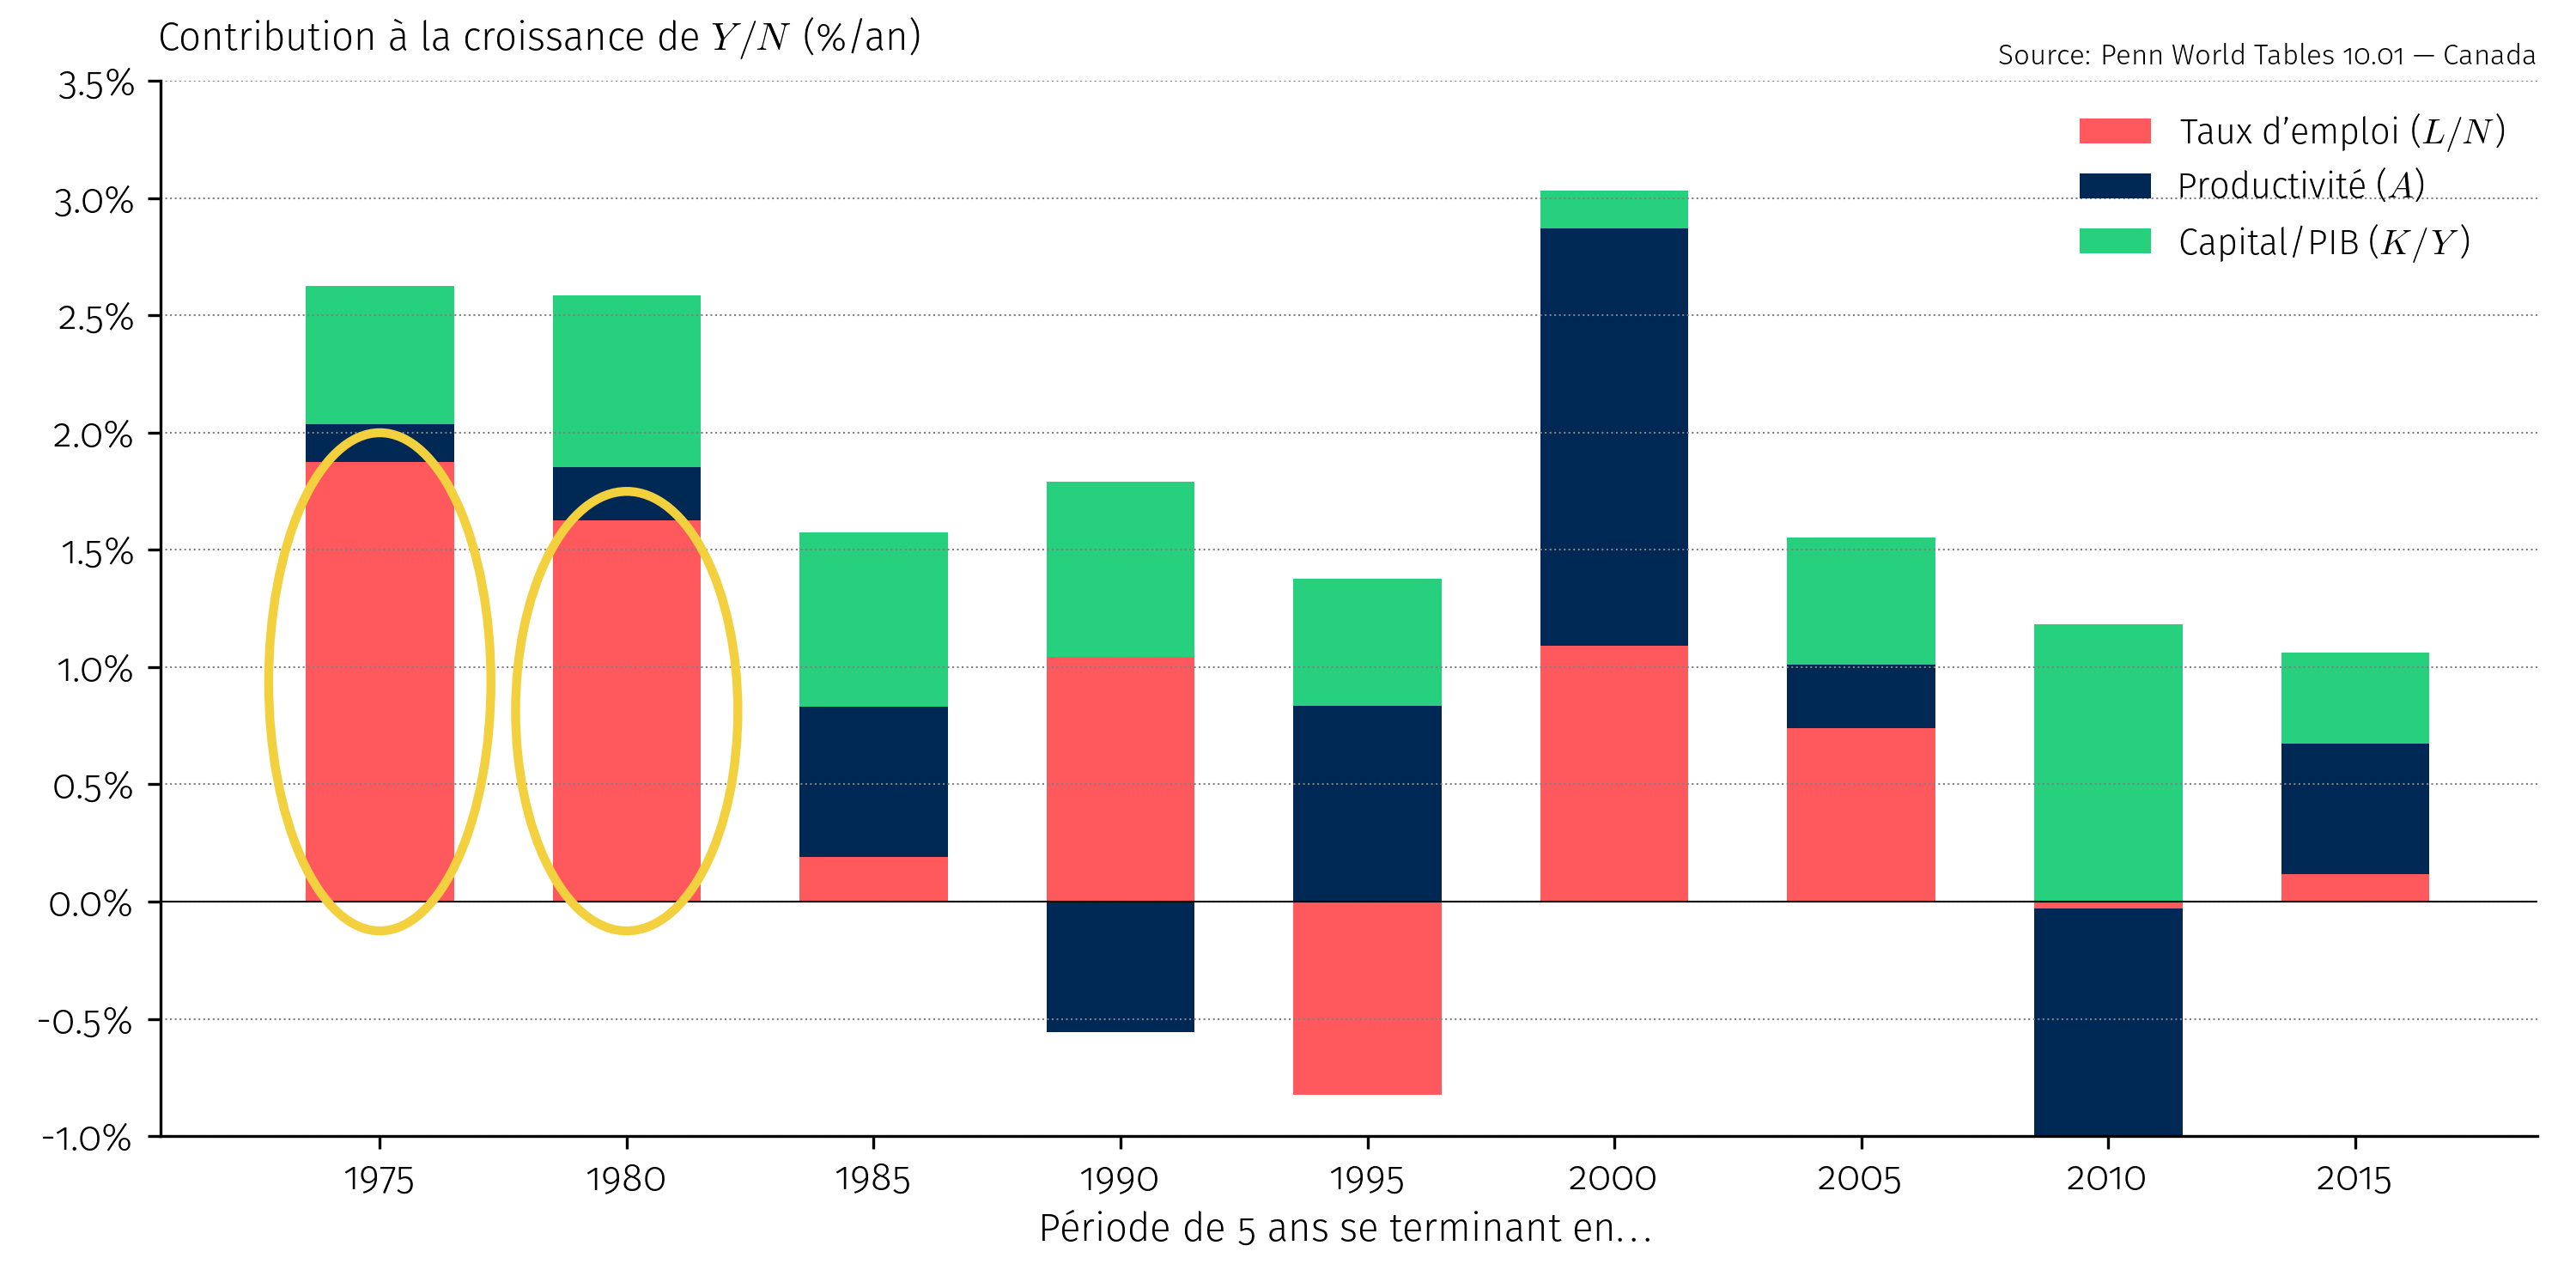
\includegraphics[width=0.95\textwidth, keepaspectratio]{canada_gdp_decomposition_5y.png}
   \end{figure}
\end{frame}

% ============================================================================
\begin{frame}{Plan}
   \begin{enumerate}
      \setlength\itemsep{0.5cm}
      \item {\color{gray!50}Théories de la productivité}
      \item \textbf{Indicateurs du marché du travail}
      \item Un modèle simple du marché du travail
      \item Applications du modèle
      \item Technologie, IA, et inégalités
   \end{enumerate}
\end{frame}

% ============================================================================
\sectionframe{Indicateurs du marché du travail}
% ============================================================================

\begin{frame}[t]{Comment mesure-t-on le marché du travail?}
   Les statistiques sur l'emploi proviennent de deux enquêtes complémentaires :
   \vspace{0.25cm}
   \begin{enumerate}
      \setlength\itemsep{0.25cm}
      \item \textbf{Enquête auprès des ménages} (Canada : \textbf{EPA}; É.-U.\ : \textbf{CPS})
      \vspace{0.15cm}
      \begin{itemize}
         \setlength\itemsep{0.15cm}
         \item $\sim$50K ménages contactés chaque mois au Canada
         \item Questions sur le statut d'emploi durant la \textit{semaine de référence}
      \end{itemize}
      \item \textbf{Enquête auprès des établissements} (Canada : \textbf{EERH}; É.-U.\ : \textbf{CES})
      \vspace{0.15cm}
      \begin{itemize}
         \setlength\itemsep{0.15cm}
         \item Compte les emplois à partir des \textbf{registres de paie} des entreprises
         \item Plus fiable pour le \textit{nombre} d'emplois, mais publiée avec délai
      \end{itemize}
   \end{enumerate}
   \vspace{0.25cm}
   Les marchés financiers réagissent fortement aux rapports mensuels sur l'emploi\ldots
\end{frame}

\begin{frame}[t]{Trois catégories}
   \small
   La population en âge de travailler se divise en trois groupes :
   \vspace{0.2cm}
   \begin{center}
   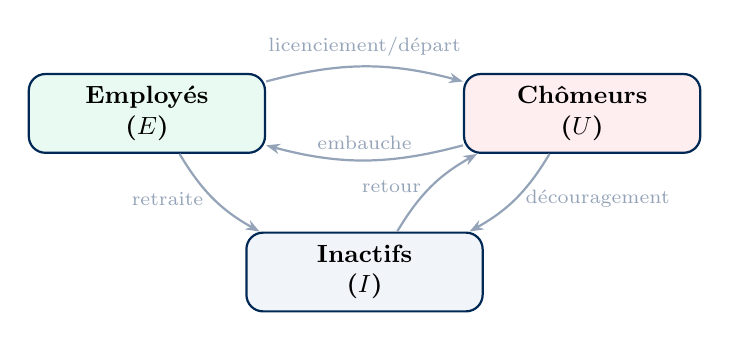
\begin{tikzpicture}[
      node distance=1.5cm,
      box/.style={draw=HECnavy, rounded corners=6pt, thick, minimum width=3cm,
                  minimum height=1cm, align=center, font=\small\bfseries},
      arr/.style={-{Stealth[length=5pt]}, thick, HECgray}
   ]
      \node[box, fill=HECgreen!10] (E) {Employés\\($E$)};
      \node[box, fill=HECcoral!10, right=2.5cm of E] (U) {Chômeurs\\($U$)};
      \node[box, fill=HEClightgray, below=1.5cm of $(E)!0.5!(U)$] (I) {Inactifs\\($I$)};

      \draw[arr, bend left=15] (E) to node[above, font=\scriptsize] {licenciement/départ} (U);
      \draw[arr, bend left=15] (U) to node[above, font=\scriptsize] {embauche} (E);
      \draw[arr, bend left=15] (U) to node[right, font=\scriptsize] {découragement} (I);
      \draw[arr, bend left=15] (I) to node[left, font=\scriptsize] {retour} (U);
      \draw[arr, bend right=15] (E) to node[left, font=\scriptsize] {retraite} (I);
   \end{tikzpicture}
   \end{center}
   \begin{defbox}
      \textbf{Chômeur :} sans emploi, disponible et en \textbf{recherche active}.
   \end{defbox}
\end{frame}

\begin{frame}[t]{Trois ratios essentiels}
   \begin{defbox}[Indicateurs du marché du travail]
      \vspace{-0.5cm}
      \begin{align*}
         \text{Taux de participation} &= \frac{E + U}{\text{Pop.\ en âge de travailler}} \times 100 \\[5pt]
         \text{Taux d'emploi} &= \frac{E}{\text{Pop.\ en âge de travailler}} \times 100 \\[5pt]
         \text{Taux de chômage} &= \frac{U}{E + U} \times 100
      \end{align*}
   \end{defbox}
\end{frame}

\begin{frame}{Le marché du travail canadien}
   \begin{figure}
      \centering
      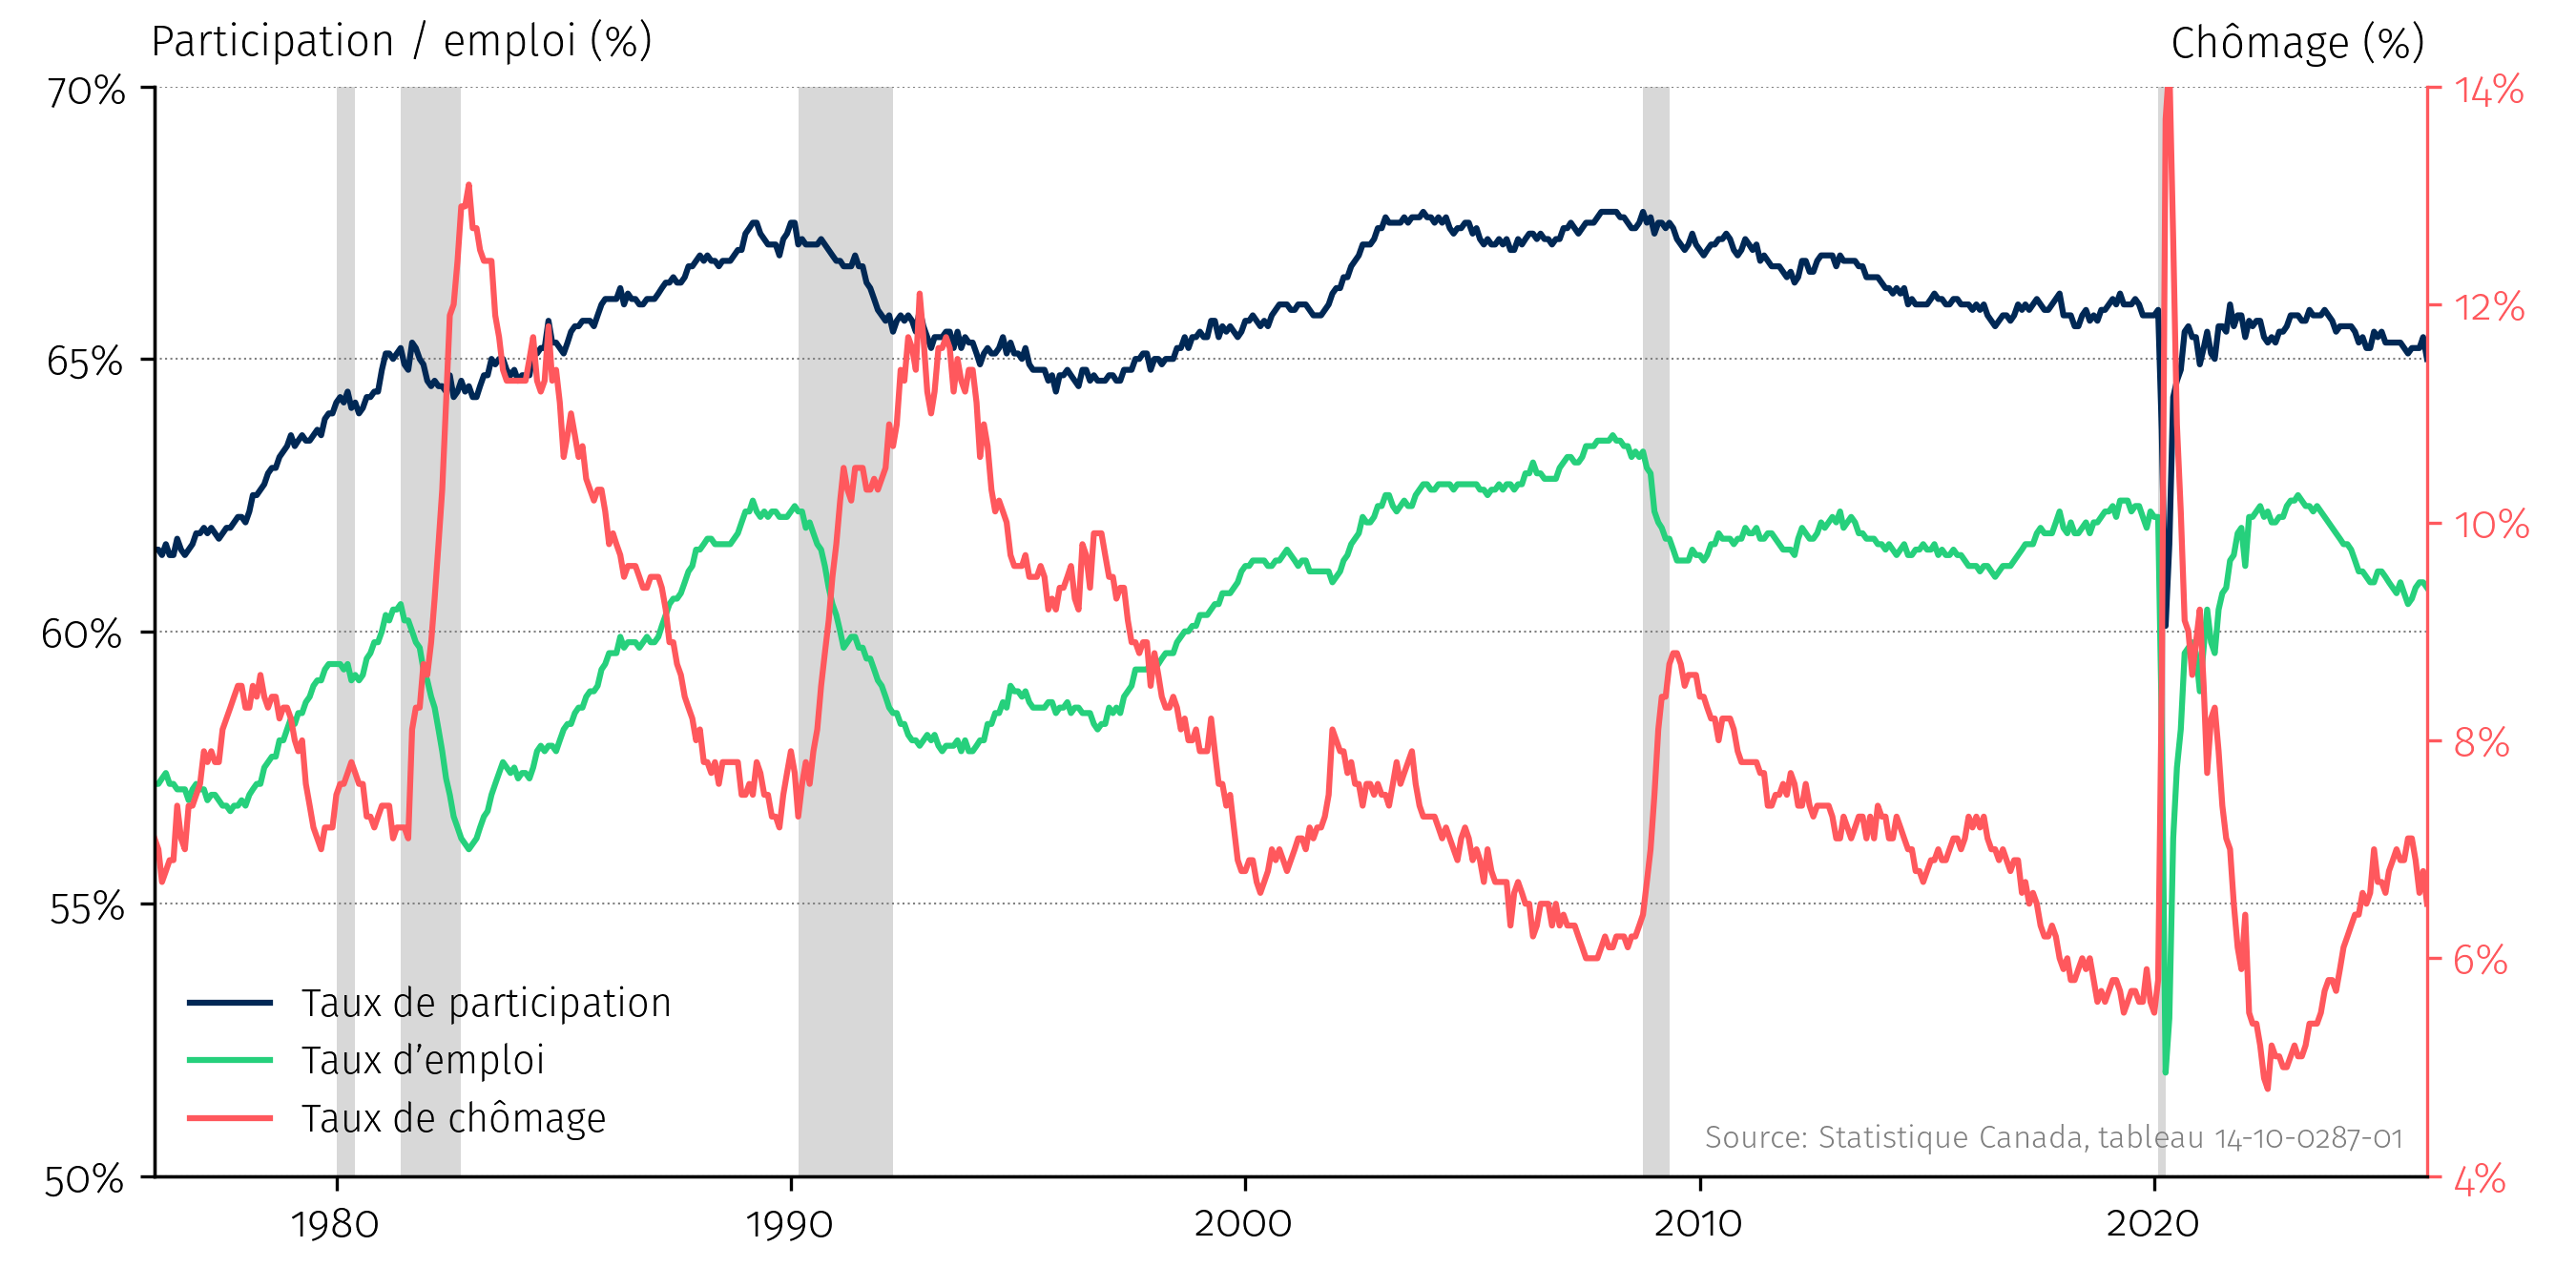
\includegraphics[width=0.95\textwidth]{labor_market_indicators_ca.png}
   \end{figure}
\end{frame}

\begin{frame}[t]{Pourquoi le taux de chômage ne suffit-il pas?}
   \footnotesize
   \vspace{-0.2cm}
   \begin{warning}[Limites du taux de chômage]
      \vspace{-0.4cm}
      \begin{itemize}
         \setlength\itemsep{0.07cm}
         \item \textbf{Travailleurs découragés :} une baisse du chômage peut refléter des \textit{retraits} du marché, non pas des embauches
         \item \textbf{Sous-emploi :} travail à temps partiel faute de trouver un emploi à temps plein
         \item \textbf{Qualité des emplois :} un taux très faible peut signifier que les travailleurs n'ont pas les ressources pour chercher assez longtemps afin de trouver un bon \textit{match}
         \item \textbf{Démographie :} le vieillissement fait baisser le chômage (les retraités quittent la population active) sans amélioration réelle du marché du travail
      \end{itemize}
   \end{warning}
   \vspace{0.05cm}
   \begin{bizimplication}
      Pour évaluer la santé réelle du marché du travail, regardez le taux de participation, le taux d'emploi \textbf{et} les mesures de sous-emploi (U-6 aux États-Unis).
   \end{bizimplication}
\end{frame}

\begin{frame}[t]{Les conséquences du chômage}
   \small
   Perdre son emploi est très \textbf{coûteux} :
   \vspace{0.25cm}
   \begin{itemize}
      \setlength\itemsep{0.25cm}
      \item 10--20\% de pertes de \textbf{revenus à vie} et risque accru de mortalité accru
      \item Principalement dû à des \textbf{salaires plus bas}, moins à une baisse de l’emploi
      \item Particulièrement coûteux en \textbf{récession}
   \end{itemize}
   \vspace{0.5cm}
   \textbf{Pourquoi} le chômage est-il si coûteux?
   \vspace{0.25cm}
   \begin{itemize}
      \setlength\itemsep{0.25cm}
      \item Perte de \textbf{capital humain} spécifique à l’entreprise
      \item Perte de \textbf{sécurité d’emploi} (le chômage engendre le chômage)
   \end{itemize}
\end{frame}

\begin{frame}{De la mesure à l'interprétation}
   Nous pouvons \textit{mesurer} le marché du travail avec précision.
   \vspace{0.3cm}

   Mais qu'est-ce qui \textbf{détermine} le niveau d'emploi et les salaires?
   \vspace{0.3cm}

   \begin{itemize}
      \setlength\itemsep{0.2cm}
      \item Devrait-on augmenter le salaire minimum?
      \item Quelles sont les causes de l'augmentation des inégalités salariales?
      \item Est-ce que les impôts sur le revenu sont trop élevés?
      \item Comment l'immigration affecte-t-elle le marché du travail?
   \end{itemize}
   \vspace{0.3cm}
   Pour répondre, il nous faut un modèle $\to$ \textbf{offre et demande de travail}
\end{frame}

% ============================================================================
\begin{frame}{Plan}
   \begin{enumerate}
      \setlength\itemsep{0.5cm}
      \item {\color{gray!50}Théories de la productivité}
      \item {\color{gray!50}Indicateurs du marché du travail}
      \item \textbf{Un modèle simple du marché du travail}
      \item Applications du modèle
      \item Technologie, IA, et inégalités
   \end{enumerate}
\end{frame}

% ============================================================================
\sectionframe{Un modèle simple du marché du travail}
% ============================================================================

\begin{frame}[t]{L'offre de travail}
   \begin{columns}[T]
      \begin{column}{0.5\textwidth}
         \vspace{0.5cm}
         \textbf{Pente positive :} un salaire réel plus élevé incite au travail (ceteris paribus). \\ \vspace{0.5cm}

         \textbf{Déterminants (déplacements) :}
         \vspace{0.15cm}
         \begin{itemize}
            \setlength\itemsep{0.15cm}
            \item \textbf{Démographie}
            \item \textbf{Impôts sur le revenu}
            \item \textbf{Richesse} (effet de revenu)
         \end{itemize}
      \end{column}
      \begin{column}{0.46\textwidth}
         \centering
         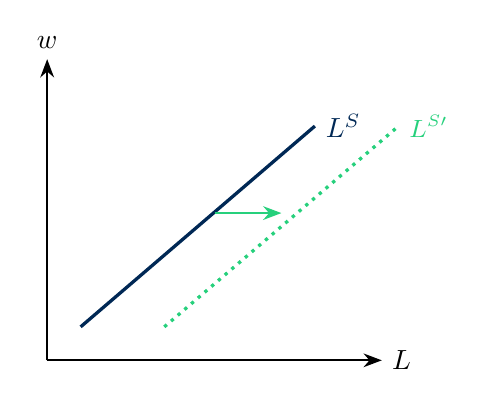
\begin{tikzpicture}[scale=0.85]
            \draw[-{Stealth}, thick] (0,0) -- (5,0) node[right] {$L$};
            \draw[-{Stealth}, thick] (0,0) -- (0,4.5) node[above] {$w$};
            \draw[HECnavy, very thick] (0.5,0.5) -- (4,3.5) node[right] {$L^S$};
            \draw[HECgreen, very thick, dotted] (1.75,0.5) -- (5.25,3.5)
               node[right, font=\small] {$L^{S\prime}$};
            \draw[-{Stealth}, HECgreen, thick] (2.5,2.2) -- (3.5,2.2);
         \end{tikzpicture}
         \vspace{0.1cm}

         {\footnotesize\textcolor{HECgray}{$\uparrow$ population $\to$ $L^S$ se déplace à droite}}
      \end{column}
   \end{columns}
\end{frame}

\begin{frame}[t]{La demande de travail}
   \begin{columns}[T]
      \begin{column}{0.5\textwidth}
         \vspace{0.5cm}
         \textbf{Pente négative :} un salaire réel plus élevé réduit la demande de travail. \\ \vspace{0.5cm}

         \textbf{Déterminants (déplacements) :}
         \vspace{0.15cm}
         \begin{itemize}
            \setlength\itemsep{0.15cm}
            \item \textbf{Cycle économique}
            \item \textbf{Impôts sur la masse salariale}
            \item \textbf{Coût du capital}
            \item \textbf{Productivité de la main d'{\oe}uvre}
         \end{itemize}
      \end{column}
      \begin{column}{0.46\textwidth}
         \centering
         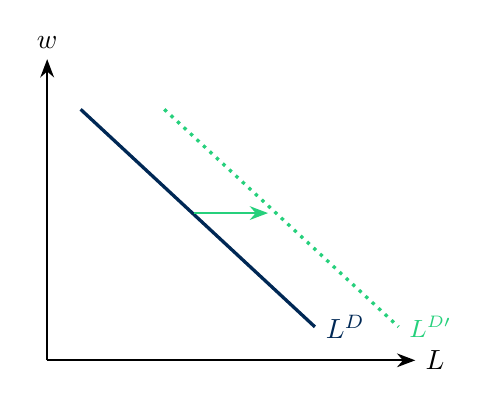
\begin{tikzpicture}[scale=0.85]
            \draw[-{Stealth}, thick] (0,0) -- (5.5,0) node[right] {$L$};
            \draw[-{Stealth}, thick] (0,0) -- (0,4.5) node[above] {$w$};
            \draw[HECnavy, very thick] (0.5,3.75) -- (4,0.5) node[right] {$L^D$};
            \draw[HECgreen, very thick, dotted] (1.75,3.75) -- (5.25,0.5)
               node[right, font=\small] {$L^{D\prime}$};
            \draw[-{Stealth}, HECgreen, thick] (2.2,2.2) -- (3.3,2.2);
         \end{tikzpicture}
         \vspace{0.1cm}

         {\footnotesize\textcolor{HECgray}{$\uparrow$ productivité $\to$ $L^D$ se déplace à droite}}
      \end{column}
   \end{columns}
\end{frame}

\begin{frame}[t]{L'équilibre de plein emploi}
   \begin{columns}[T]
      \begin{column}{0.48\textwidth}
         L'intersection donne :
         \vspace{0.15cm}
         \begin{itemize}
            \setlength\itemsep{0.15cm}
            \item $L^* =$ emploi d'équilibre
            \item $w^* =$ salaire \textit{réel} d'équilibre
         \end{itemize}
         \vspace{0.2cm}
         \begin{keyinsight}
            À l'équilibre, le salaire s'ajuste de sorte que ceux qui veulent travailler trouvent un emploi.
         \end{keyinsight}
      \end{column}
      \begin{column}{0.48\textwidth}
         \centering
         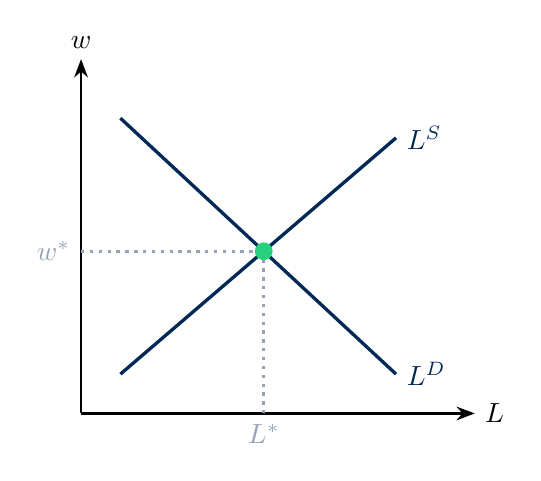
\begin{tikzpicture}[scale=1]
            \draw[-{Stealth}, thick] (0,0) -- (5,0) node[right] {$L$};
            \draw[-{Stealth}, thick] (0,0) -- (0,4.5) node[above] {$w$};
            \draw[HECnavy, very thick] (0.5,0.5) -- (4,3.5) node[right] {$L^S$};
            \draw[HECnavy, very thick] (0.5,3.75) -- (4,0.5) node[right] {$L^D$};
            % Intersection at (2.32, 2.06)
            \draw[dotted, very thick, HECgray] (2.32,0) node[below] {$L^*$} -- (2.32,2.06);
            \draw[dotted, very thick, HECgray] (0,2.06) node[left] {$w^*$} -- (2.32,2.06);
            \filldraw[HECgreen] (2.32,2.06) circle (3pt);
         \end{tikzpicture}
      \end{column}
   \end{columns}
\end{frame}

\begin{frame}{À quoi correspond le chômage?}
   \centering
   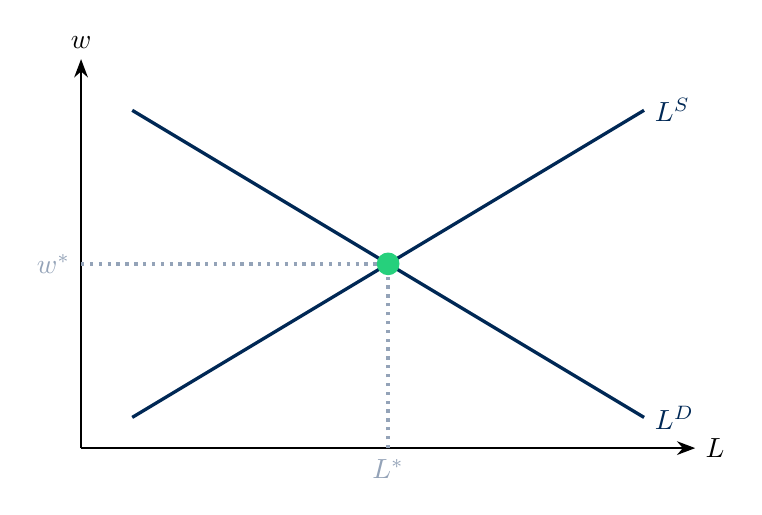
\begin{tikzpicture}[scale=1.3]
      \draw[-{Stealth}, thick] (0,0) -- (6,0) node[right] {$L$};
      \draw[-{Stealth}, thick] (0,0) -- (0,3.8) node[above] {$w$};
      \draw[HECnavy, very thick] (0.5,0.3) -- (5.5,3.3) node[right] {$L^S$};
      \draw[HECnavy, very thick] (0.5,3.3) -- (5.5,0.3) node[right] {$L^D$};
      % Intersection at (3.0, 1.8)
      \draw[dotted, very thick, HECgray] (3.0,0) node[below] {$L^*$} -- (3.0,1.8);
      \draw[dotted, very thick, HECgray] (0,1.8) node[left] {$w^*$} -- (3.0,1.8);
      \filldraw[HECgreen] (3.0,1.8) circle (3pt);
   \end{tikzpicture}
\end{frame}

\begin{frame}{À quoi correspond le chômage?}
   \centering
   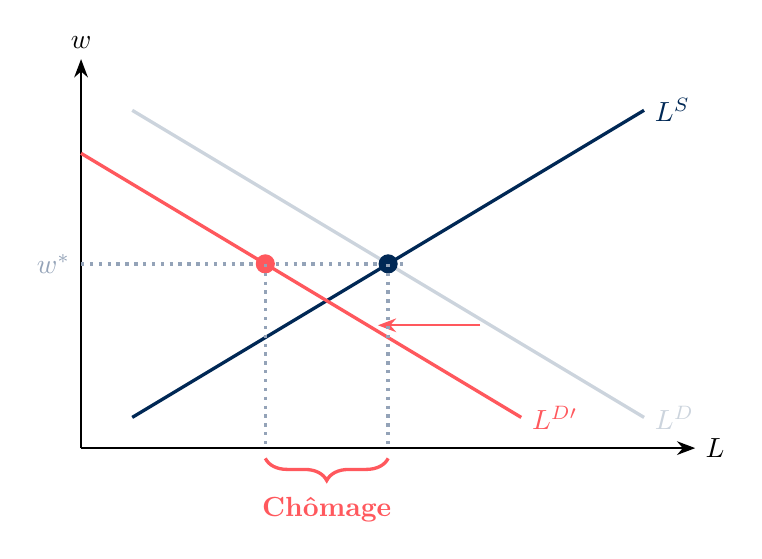
\begin{tikzpicture}[scale=1.3]
      % Axes
      \draw[-{Stealth}, thick] (0,0) -- (6,0) node[right] {$L$};
      \draw[-{Stealth}, thick] (0,0) -- (0,3.8) node[above] {$w$};
      % Supply curve
      \draw[HECnavy, very thick] (0.5,0.3) -- (5.5,3.3) node[right] {$L^S$};
      % Original demand (faded dashed)
      \draw[HECnavy!20, very thick] (0.5,3.3) -- (5.5,0.3) node[right] {$L^D$};
      % Shifted demand (left by 1.2): w = 2.88 - 0.6L
      \draw[HECcoral, very thick] (0,2.88) -- (4.3,0.3) node[right] {$L^{D\prime}$};
      % Shift arrow between the two demand curves
      \draw[-{Stealth}, HECcoral, thick] (3.9,1.2) -- (2.9,1.2);
      % Rigid wage: horizontal dashed line at w*
      \draw[HECgray, dotted, very thick] (0,1.8) node[left] {$w^*$} -- (3.2,1.8);
      % Intersection points at w*
      \filldraw[HECcoral] (1.8,1.8) circle (2.5pt);   % on new demand: L_D = 1.8
      \filldraw[HECnavy] (3.0,1.8) circle (2.5pt);    % on supply: L_S = 3.0
      % Vertical dotted lines to x-axis
      \draw[dotted, very thick, HECgray] (1.8,1.8) -- (1.8,0);
      \draw[dotted, very thick, HECgray] (3.0,1.8) -- (3.0,0);
      % Underbrace for unemployment gap
      \draw [decorate, decoration={brace, amplitude=8pt, mirror}, very thick, HECcoral]
         (1.8, -0.1) -- (3.0, -0.1)
         node [midway, below=10pt, HECcoral] {\textbf{Chômage}};
   \end{tikzpicture}
\end{frame}

\begin{frame}{Le modèle en action}
   On utilise maintenant ce modèle pour analyser \textbf{quatre phénomènes réels} :
   \vspace{0.3cm}
   \begin{enumerate}
      \setlength\itemsep{0.25cm}
      \item La participation des femmes au marché du travail
      \item Le vieillissement démographique
      \item L'immigration
      \item Le rôle de l'inflation en récession
   \end{enumerate}
   \vspace{0.3cm}
   Dans chaque cas : Quelle courbe se déplace? Quel effet sur $w$ et $L$? CT vs.\ LT?
\end{frame}

% ============================================================================
\begin{frame}{Plan}
   \begin{enumerate}
      \setlength\itemsep{0.5cm}
      \item {\color{gray!50}Théories de la productivité}
      \item {\color{gray!50}Indicateurs du marché du travail}
      \item {\color{gray!50}Un modèle simple du marché du travail}
      \item \textbf{Applications du modèle}
      \item Technologie, IA, et inégalités
   \end{enumerate}
\end{frame}

% ============================================================================
\sectionframe{Applications du modèle}
% ============================================================================

\begin{frame}[t]{Deux horizons temporels}
   \begin{columns}[T]
      \begin{column}{0.48\textwidth}
         \textbf{\textcolor{HECcoral}{\quad Court terme ($\sim$1 an)}}
         \vspace{0.1cm}
         \begin{itemize}
            \setlength\itemsep{0.1cm}
            \item Le capital ($K$) est \textbf{fixe}
            \item Seul le travail s'ajuste
            \item Un choc d'offre sur $L^S$ (ex.\ immigration) n'affecte pas $L^D$
         \end{itemize}
      \end{column}
      \begin{column}{0.48\textwidth}
         \textbf{\textcolor{HECnavy}{\quad Long terme ($\sim$5+ ans)}}
         \vspace{0.1cm}
         \begin{itemize}
            \setlength\itemsep{0.1cm}
            \item Le capital \textbf{s'ajuste} (Solow!)
            \item Plus de travailleurs $\to$ rendement du capital $\uparrow$ $\to$ investissement $\uparrow$
            \item $K \uparrow$ $\to$ $L^D$ se déplace à droite
         \end{itemize}
      \end{column}
   \end{columns}
   \vspace{0.3cm}
   \begin{defbox}[Horizon d'ajustement]
      \textbf{Court terme :} $K$ est fixe, seul $L$ s'ajuste. \\
      \textbf{Long terme :} $K$ s'ajuste via le mécanisme de Solow.
   \end{defbox}
\end{frame}

% --- Application 1 : La participation des femmes ----------------------------

\begin{frame}{La révolution silencieuse}
   \begin{figure}
      \centering
      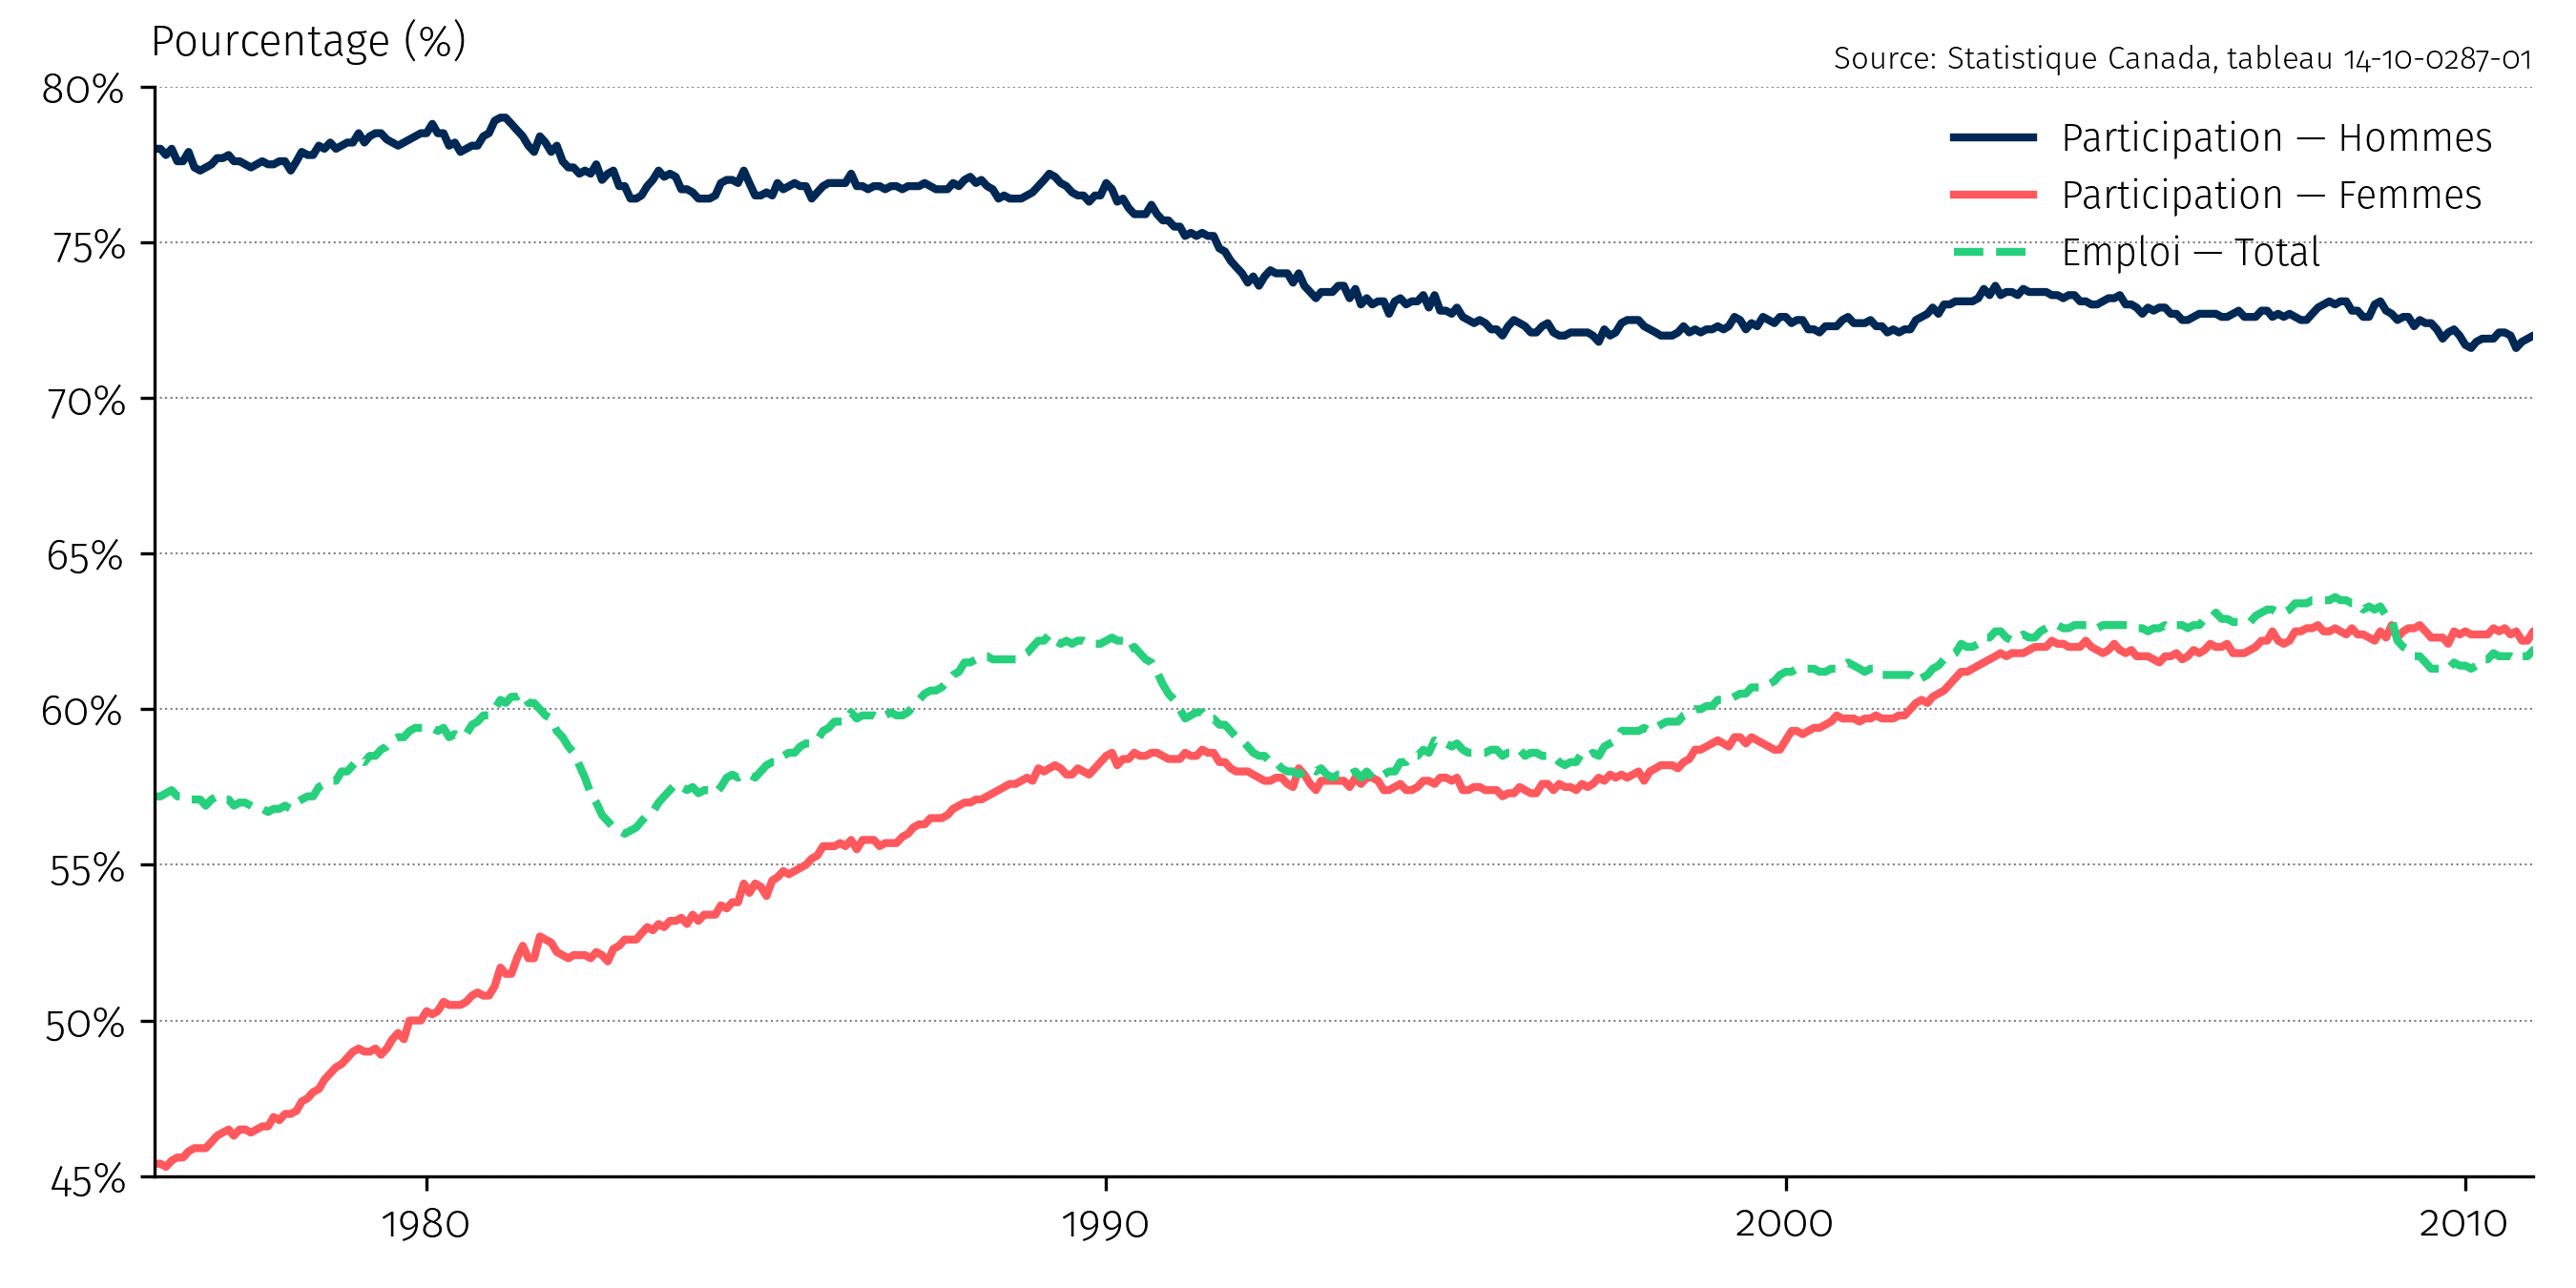
\includegraphics[width=0.95\textwidth]{participation_gender_ca.png}
   \end{figure}
\end{frame}

\begin{frame}{Participation des femmes : le modèle}
   \begin{columns}[c]
      \begin{column}{0.52\textwidth}
         \centering
         {\small\textbf{\textcolor{HECcoral}{Court terme} --- $K$ fixe}}
         \par\smallskip
         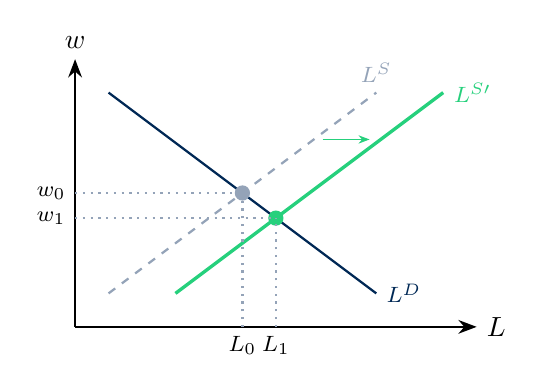
\begin{tikzpicture}[scale=0.85]
            % Axes
            \draw[-{Stealth}, thick] (0,0) -- (6,0) node[right] {$L$};
            \draw[-{Stealth}, thick] (0,0) -- (0,4) node[above] {$w$};
            % Original supply (dashed gray): y = 0.75x + 0.125
            \draw[HECgray, dashed, thick] (0.5,0.5) -- (4.5,3.5)
               node[above, font=\footnotesize] {$L^S$};
            % Demand (navy solid): y = -0.75x + 3.875
            \draw[HECnavy, thick] (0.5,3.5) -- (4.5,0.5)
               node[right, font=\footnotesize] {$L^D$};
            % Shifted supply (green, +1.0 right): y = 0.75x - 0.625
            \draw[HECgreen, very thick] (1.5,0.5) -- (5.5,3.5)
               node[right, font=\footnotesize] {$L^{S\prime}$};
            % E0: (2.5, 2.0)
            \filldraw[HECgray] (2.5,2.0) circle (3pt);
            % E1: (3.0, 1.625)
            \filldraw[HECgreen] (3.0,1.625) circle (3pt);
            % Dotted lines to x-axis
            \draw[dotted, thick, HECgray] (2.5,0) -- (2.5,2.0);
            \draw[dotted, thick, HECgray] (3.0,0) -- (3.0,1.625);
            \node[font=\footnotesize, below] at (2.5,0) {$L_0$};
            \node[font=\footnotesize, below] at (3.0,0) {$L_1$};
            % Dotted lines to y-axis (wages)
            \draw[dotted, thick, HECgray] (0,2.0) -- (2.5,2.0);
            \draw[dotted, thick, HECgray] (0,1.625) -- (3.0,1.625);
            \node[font=\footnotesize, left] at (0,2.0) {$w_0$};
            \node[font=\footnotesize, left] at (0,1.625) {$w_1$};
            % Thin shift arrow
            \draw[-{Stealth[length=4pt]}, HECgreen] (3.7,2.8) -- (4.4,2.8);
         \end{tikzpicture}
      \end{column}
      \begin{column}{0.52\textwidth}
         \centering
         {\small\textbf{\textcolor{HECnavy}{Long terme} --- $K$ s'ajuste}}
         \par\smallskip
         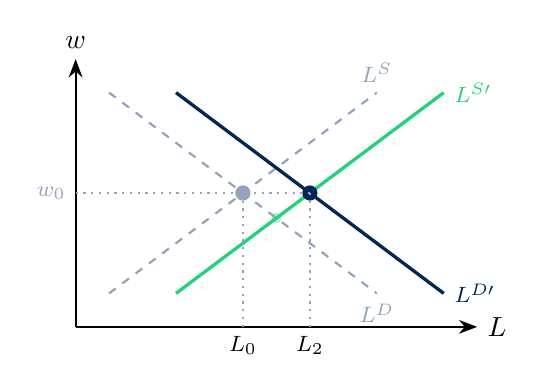
\begin{tikzpicture}[scale=0.85]
            % Axes
            \draw[-{Stealth}, thick] (0,0) -- (6,0) node[right] {$L$};
            \draw[-{Stealth}, thick] (0,0) -- (0,4) node[above] {$w$};
            % Original supply (dashed gray)
            \draw[HECgray, dashed, thick] (0.5,0.5) -- (4.5,3.5)
               node[above, font=\footnotesize] {$L^S$};
            % Original demand (dashed gray)
            \draw[HECgray, dashed, thick] (0.5,3.5) -- (4.5,0.5)
               node[below, font=\footnotesize] {$L^D$};
            % Shifted supply (green): y = 0.75x - 0.625
            \draw[HECgreen, very thick] (1.5,0.5) -- (5.5,3.5)
               node[right, font=\footnotesize] {$L^{S\prime}$};
            % Shifted demand (navy): y = -0.75x + 4.625
            \draw[HECnavy, very thick] (1.5,3.5) -- (5.5,0.5)
               node[right, font=\footnotesize] {$L^{D\prime}$};
            % E0: (2.5, 2.0)
            \filldraw[HECgray] (2.5,2.0) circle (3pt);
            % E1 faded: (3.0, 1.625)
            \filldraw[HECgreen, opacity=0.3] (3.0,1.625) circle (2pt);
            % E2: (3.5, 2.0)
            \filldraw[HECnavy] (3.5,2.0) circle (3pt);
            % Dotted lines
            \draw[dotted, thick, HECgray] (0,2.0) node[left, font=\footnotesize] {$w_0$} -- (3.5,2.0);
            \draw[dotted, thick, HECgray] (2.5,0) -- (2.5,2.0);
            \draw[dotted, thick, HECgray] (3.5,0) -- (3.5,2.0);
            \node[font=\footnotesize, below] at (2.5,0) {$L_0$};
            \node[font=\footnotesize, below] at (3.5,0) {$L_2$};
         \end{tikzpicture}
      \end{column}
   \end{columns}
\end{frame}

% --- Application 2 : Le vieillissement démographique -------------------------

\begin{frame}{Le vieillissement de la population}
   \begin{figure}
      \centering
      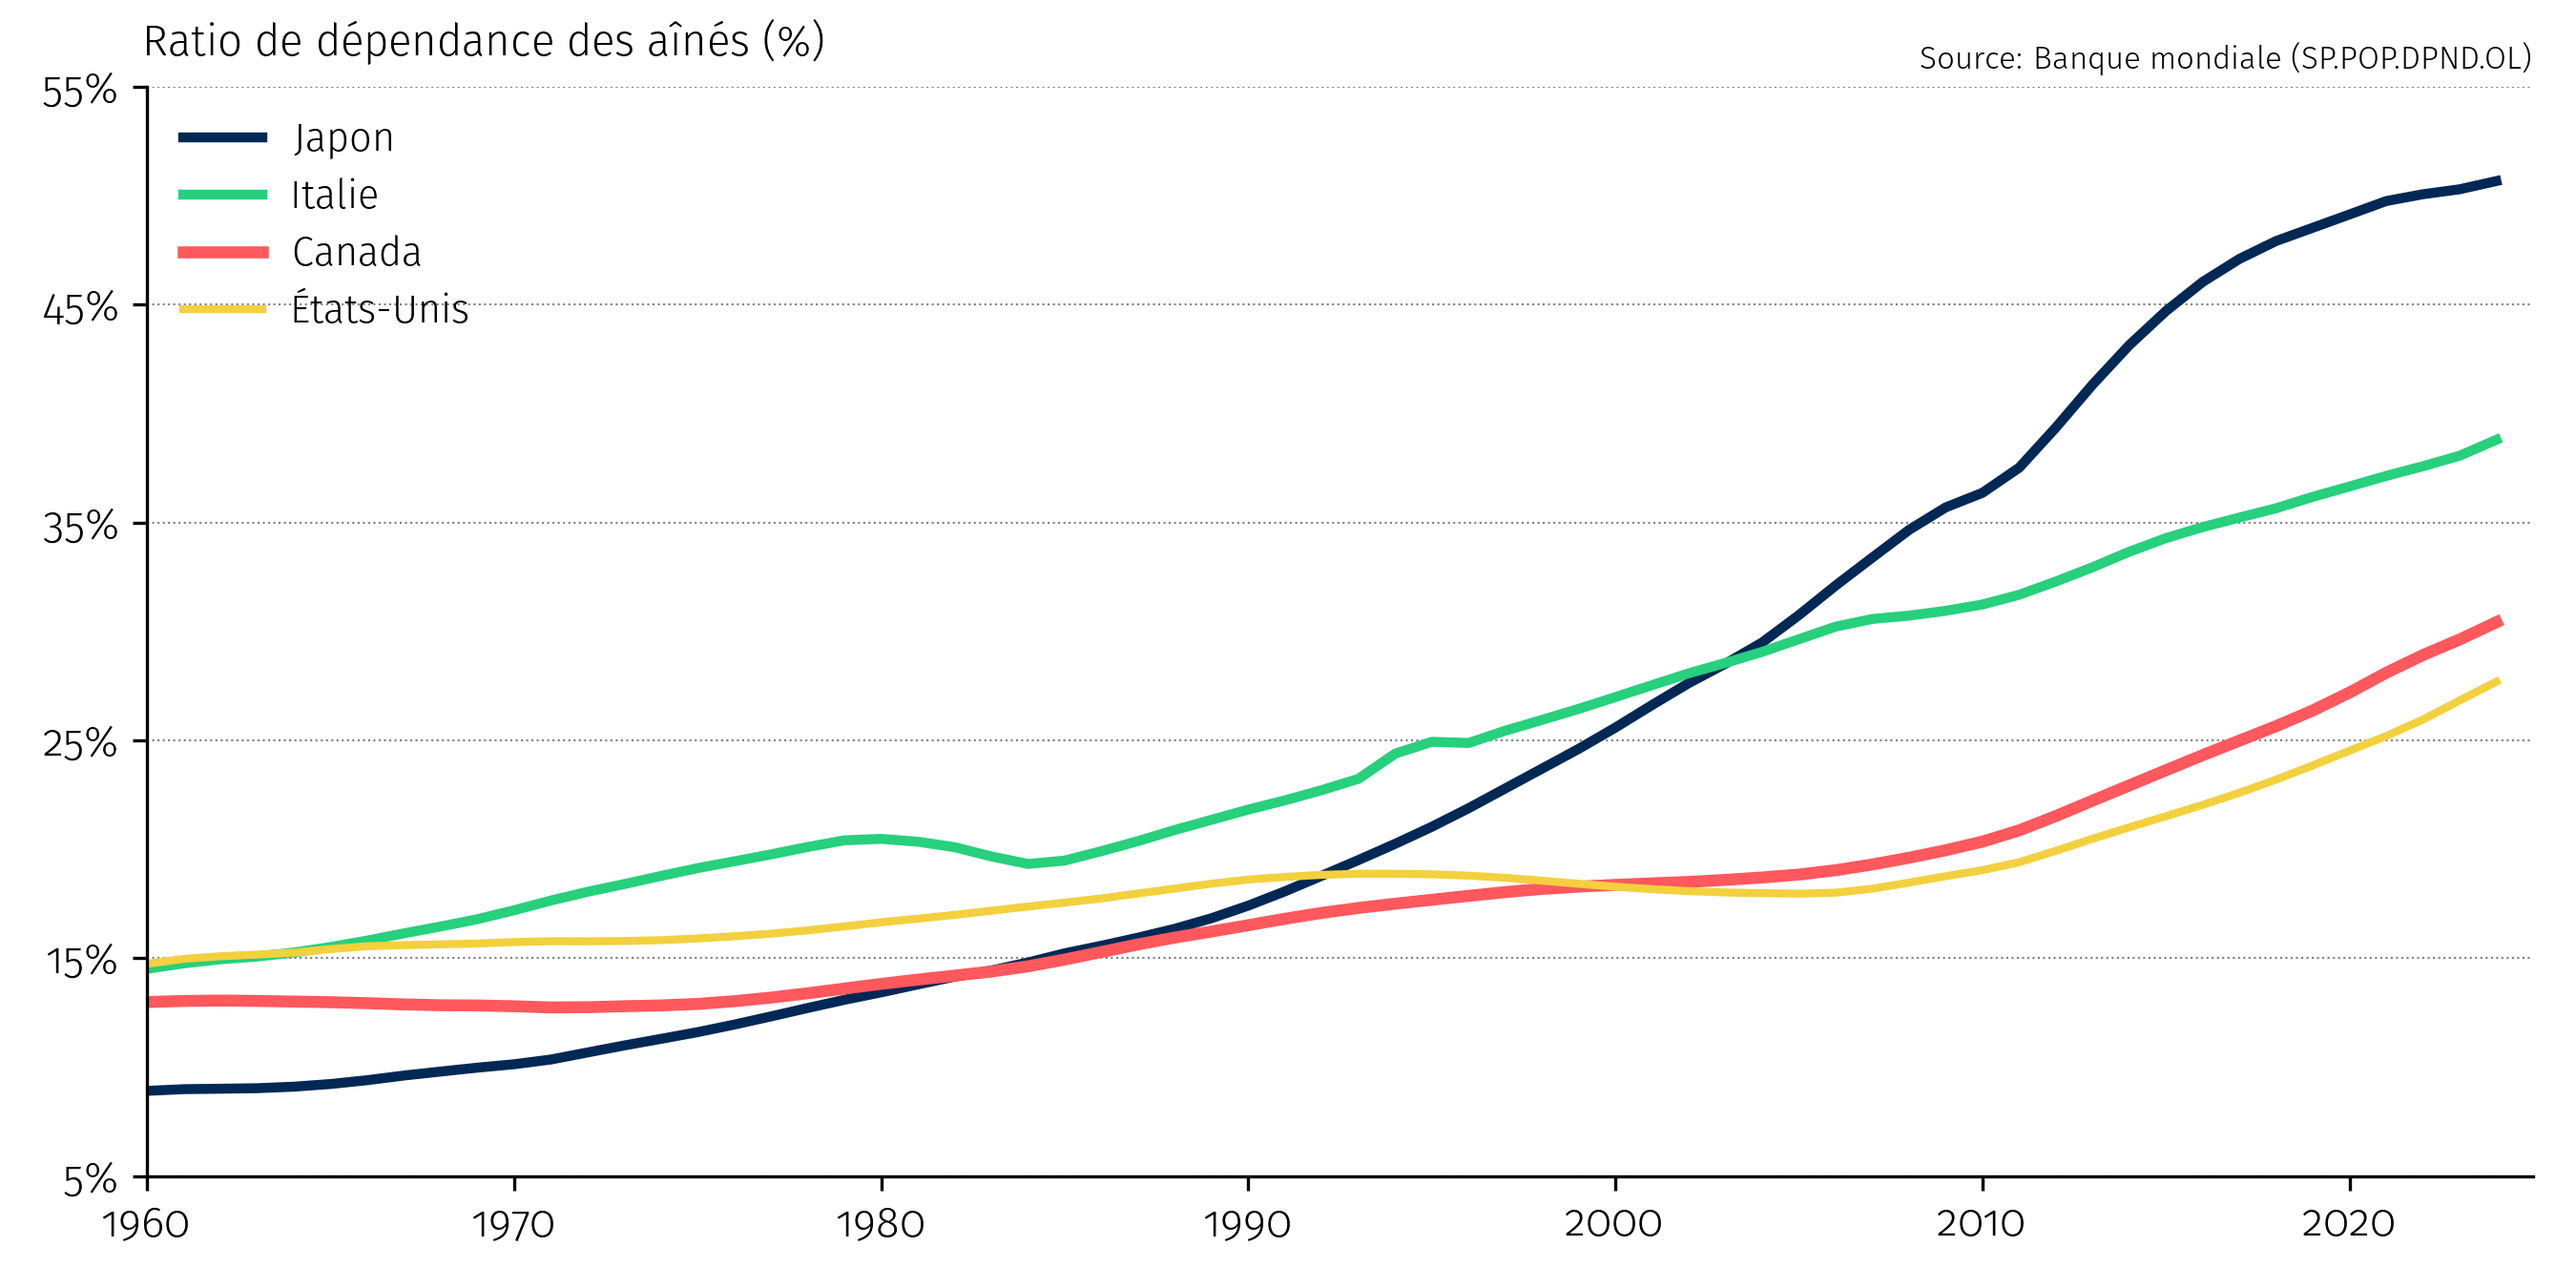
\includegraphics[width=0.95\textwidth]{aging_population.png}
   \end{figure}
\end{frame}

\begin{frame}{L'effet sur le marché du travail}
   \framesubtitle{Le taux de participation plafonne puis décline}
   \begin{figure}
      \centering
      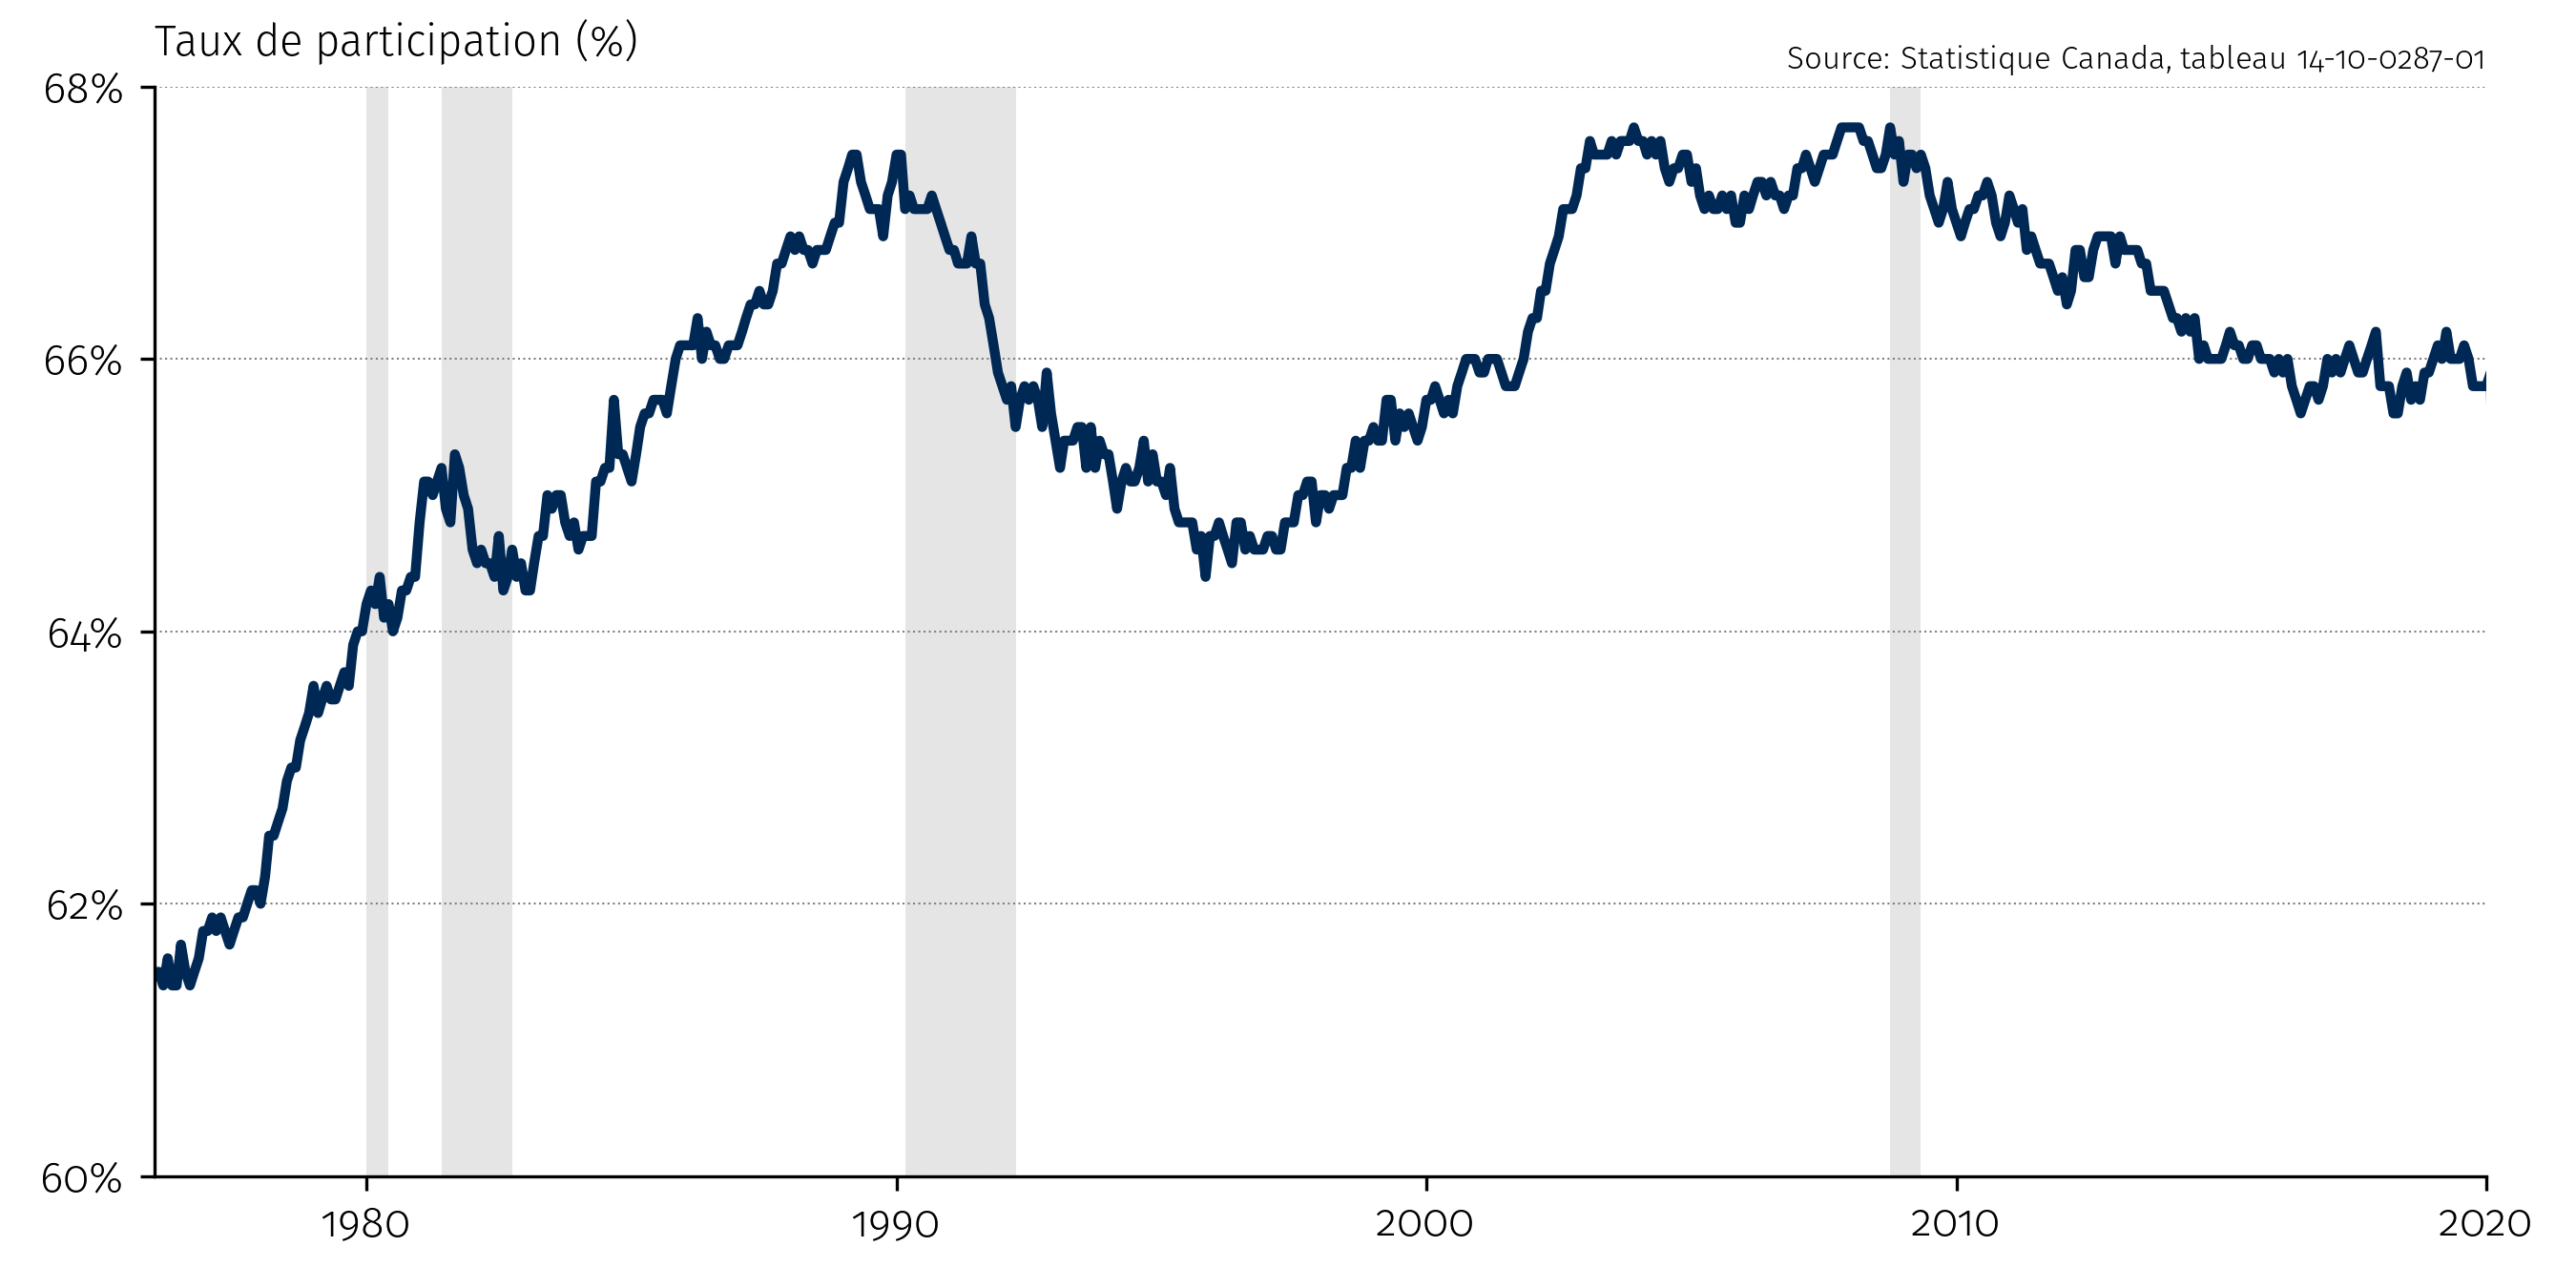
\includegraphics[width=0.95\textwidth]{participation_rate_ca.png}
   \end{figure}
\end{frame}

\begin{frame}{Vieillissement : le modèle}
   \begin{columns}[c]
      \begin{column}{0.52\textwidth}
         \centering
         {\small\textbf{\textcolor{HECcoral}{Court terme} --- $K$ fixe}}
         \par\vspace{1pt}
         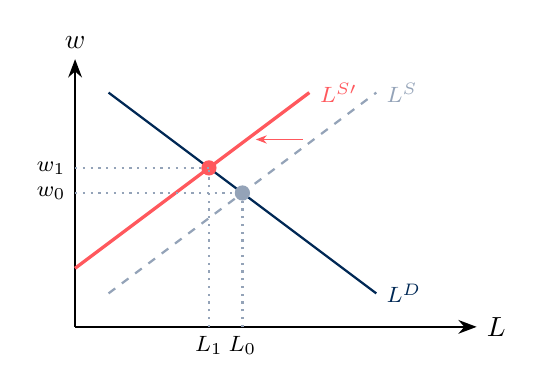
\begin{tikzpicture}[scale=0.85]
            % Axes
            \draw[-{Stealth}, thick] (0,0) -- (6,0) node[right] {$L$};
            \draw[-{Stealth}, thick] (0,0) -- (0,4) node[above] {$w$};
            % Original supply (dashed gray): y = 0.75x + 0.125
            \draw[HECgray, dashed, thick] (0.5,0.5) -- (4.5,3.5)
               node[right, font=\footnotesize] {$L^S$};
            % Demand (navy solid): y = -0.75x + 3.875
            \draw[HECnavy, thick] (0.5,3.5) -- (4.5,0.5)
               node[right, font=\footnotesize] {$L^D$};
            % Shifted supply (coral, -1.0 left): y = 0.75x + 0.875
            \draw[HECcoral, very thick] (0,0.875) -- (3.5,3.5)
               node[right, font=\footnotesize] {$L^{S\prime}$};
            % E0: (2.5, 2.0)
            \filldraw[HECgray] (2.5,2.0) circle (3pt);
            % E1: (2.0, 2.375)
            \filldraw[HECcoral] (2.0,2.375) circle (3pt);
            % Dotted lines to x-axis
            \draw[dotted, thick, HECgray] (2.5,0) -- (2.5,2.0);
            \draw[dotted, thick, HECgray] (2.0,0) -- (2.0,2.375);
            \node[font=\footnotesize, below] at (2.5,0) {$L_0$};
            \node[font=\footnotesize, below] at (2.0,0) {$L_1$};
            % Dotted lines to y-axis (wages)
            \draw[dotted, thick, HECgray] (0,2.0) -- (2.5,2.0);
            \draw[dotted, thick, HECgray] (0,2.375) -- (2.0,2.375);
            \node[font=\footnotesize, left] at (0,2.0) {$w_0$};
            \node[font=\footnotesize, left] at (0,2.375) {$w_1$};
            % Thin shift arrow
            \draw[-{Stealth[length=4pt]}, HECcoral] (3.4,2.8) -- (2.7,2.8);
         \end{tikzpicture}
      \end{column}
      \begin{column}{0.52\textwidth}
         \centering
         {\small\textbf{\textcolor{HECnavy}{Long terme} --- $K$ s'ajuste}}
         \par\vspace{1pt}
         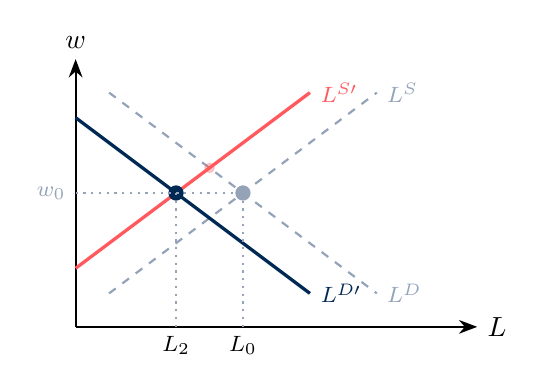
\begin{tikzpicture}[scale=0.85]
            % Axes
            \draw[-{Stealth}, thick] (0,0) -- (6,0) node[right] {$L$};
            \draw[-{Stealth}, thick] (0,0) -- (0,4) node[above] {$w$};
            % Original supply (dashed gray)
            \draw[HECgray, dashed, thick] (0.5,0.5) -- (4.5,3.5)
               node[right, font=\footnotesize] {$L^S$};
            % Original demand (dashed gray)
            \draw[HECgray, dashed, thick] (0.5,3.5) -- (4.5,0.5)
               node[right, font=\footnotesize] {$L^D$};
            % Shifted supply (coral, -1.0 left): clipped at x=0
            \draw[HECcoral, very thick] (0,0.875) -- (3.5,3.5)
               node[right, font=\footnotesize] {$L^{S\prime}$};
            % Shifted demand (navy, -1.0 left): clipped at x=0
            \draw[HECnavy, very thick] (0,3.125) -- (3.5,0.5)
               node[right, font=\footnotesize] {$L^{D\prime}$};
            % E0: (2.5, 2.0)
            \filldraw[HECgray] (2.5,2.0) circle (3pt);
            % E1 faded: (2.0, 2.375)
            \filldraw[HECcoral, opacity=0.3] (2.0,2.375) circle (2pt);
            % E2: (1.5, 2.0)
            \filldraw[HECnavy] (1.5,2.0) circle (3pt);
            % Dotted lines
            \draw[dotted, thick, HECgray] (0,2.0) node[left, font=\footnotesize] {$w_0$} -- (2.5,2.0);
            \draw[dotted, thick, HECgray] (2.5,0) -- (2.5,2.0);
            \draw[dotted, thick, HECgray] (1.5,0) -- (1.5,2.0);
            \node[font=\footnotesize, below] at (2.5,0) {$L_0$};
            \node[font=\footnotesize, below] at (1.5,0) {$L_2$};
         \end{tikzpicture}
      \end{column}
   \end{columns}
\end{frame}

% --- Application 3 : L'immigration -------------------------------------------

\begin{frame}{L'immigration au Canada}
   \begin{figure}
      \centering
      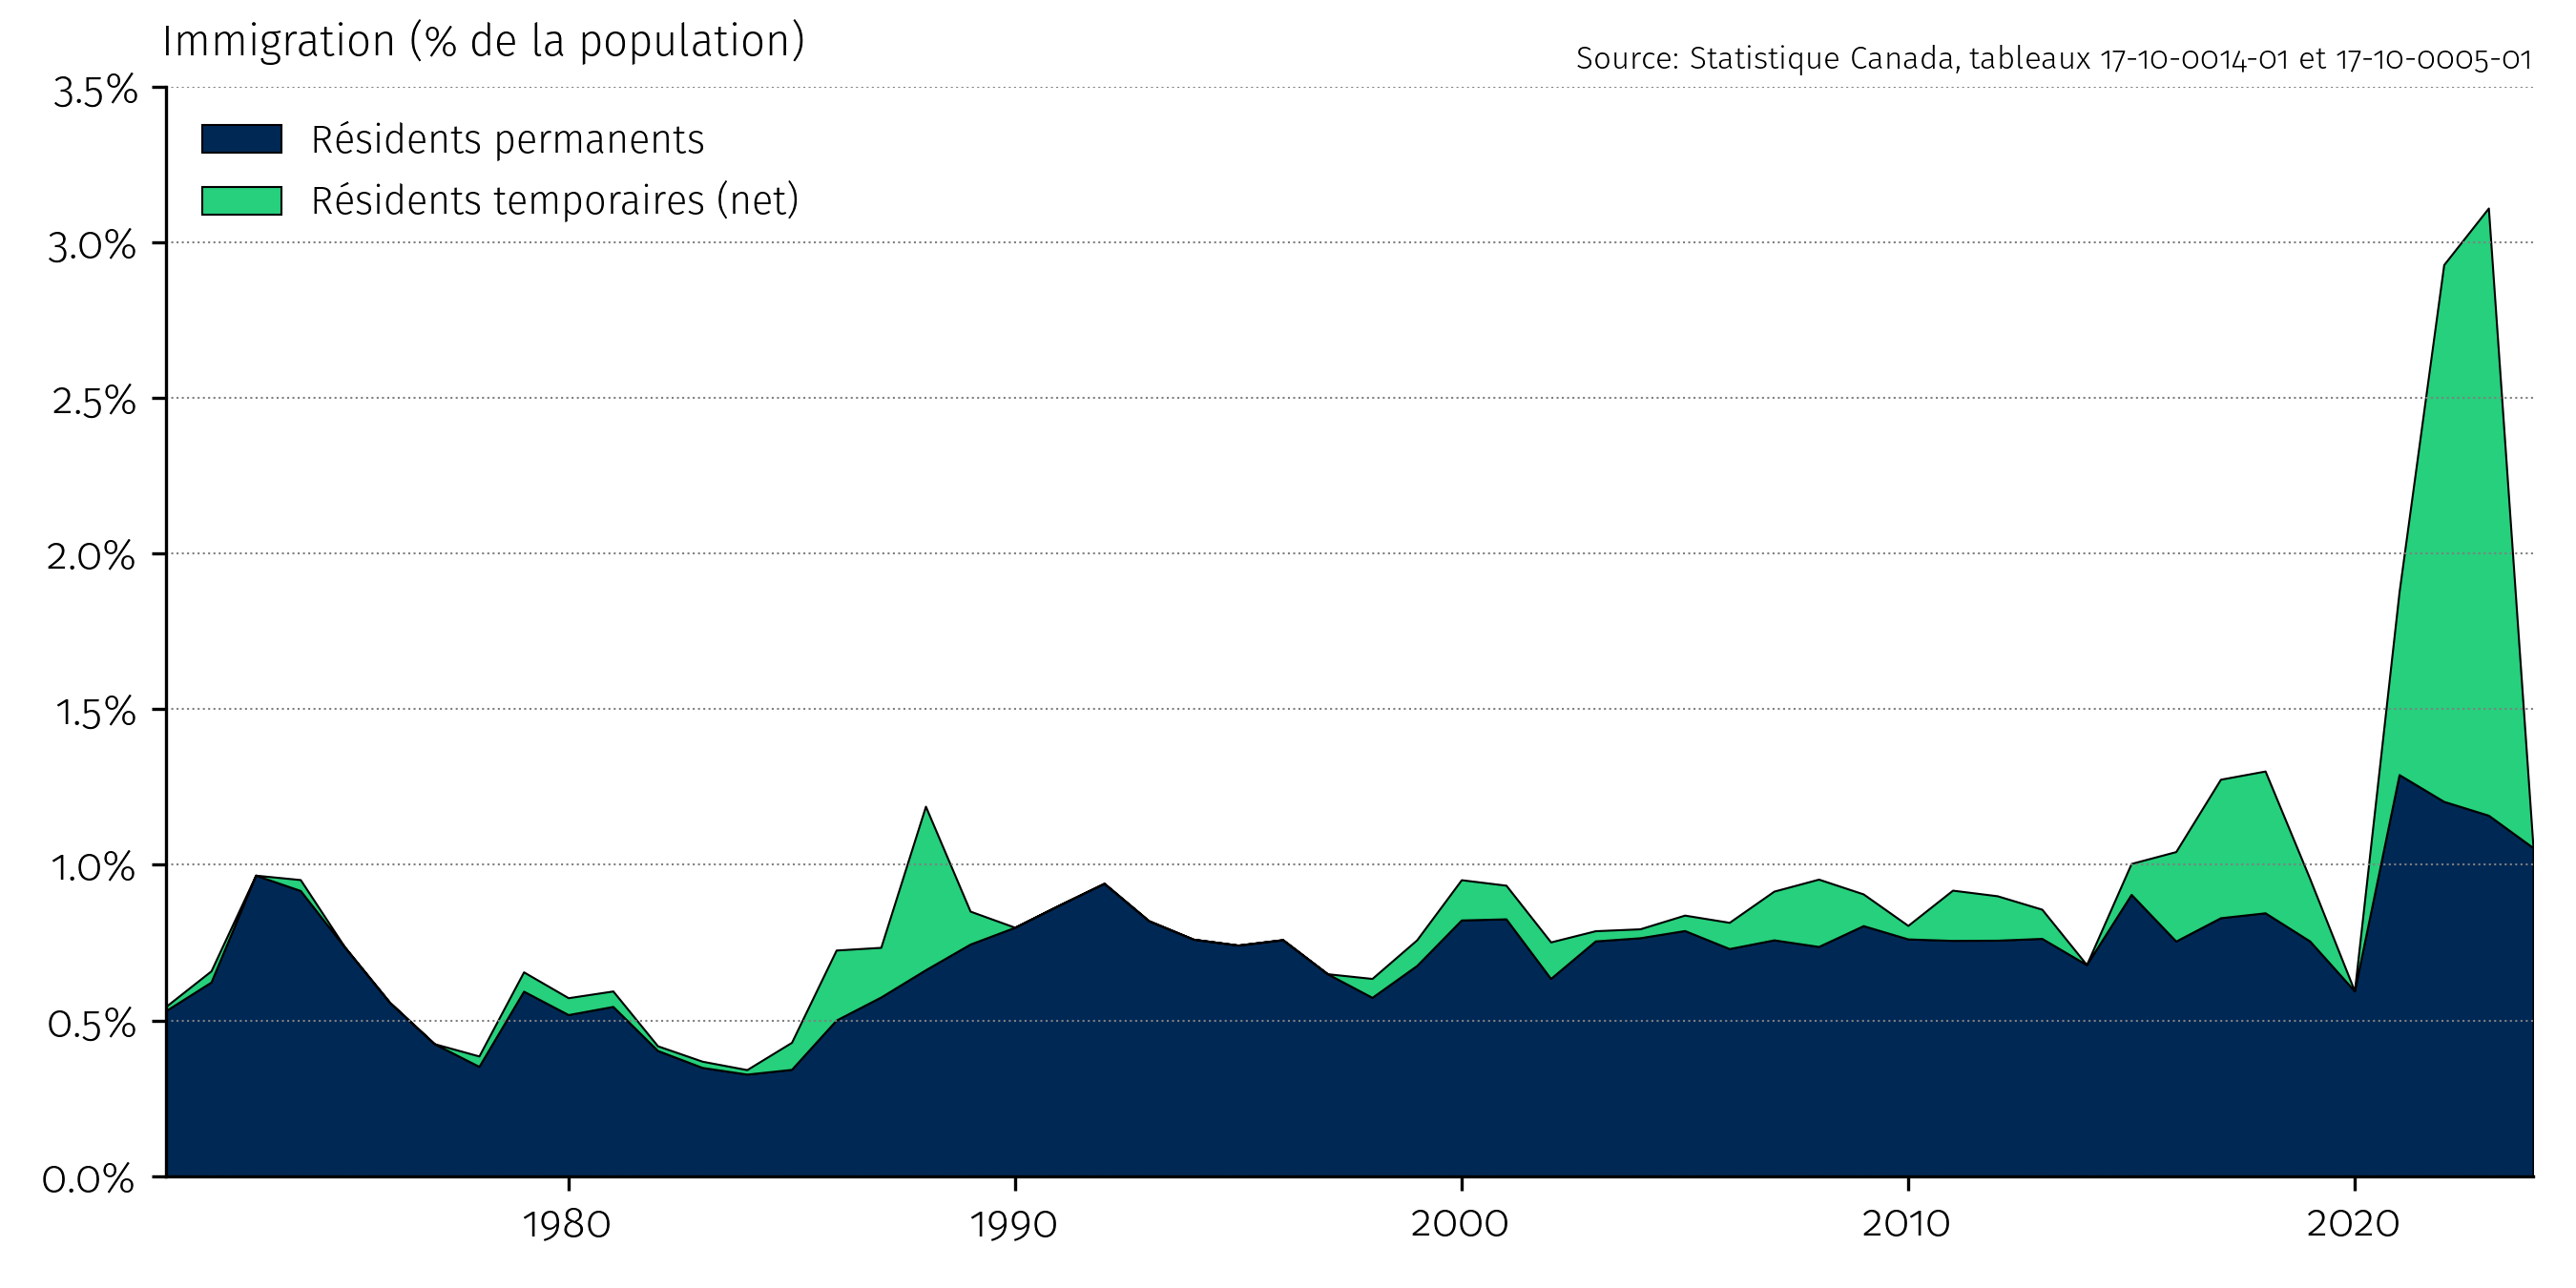
\includegraphics[width=0.95\textwidth]{immigration_ca.png}
   \end{figure}
\end{frame}

\begin{frame}{Immigration : le modèle}
   \begin{columns}[c]
      \begin{column}{0.52\textwidth}
         \centering
         {\small\textbf{\textcolor{HECcoral}{Court terme} --- $K$ fixe}}
         \par\vspace{1pt}
         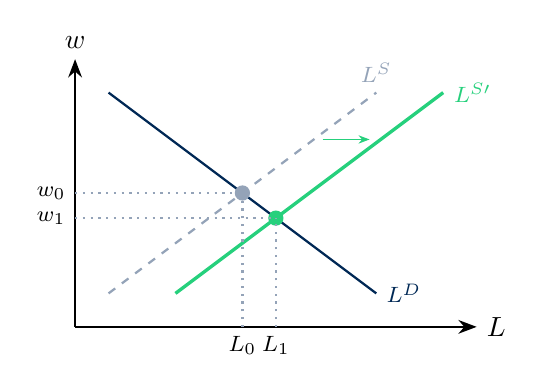
\begin{tikzpicture}[scale=0.85]
            % Axes
            \draw[-{Stealth}, thick] (0,0) -- (6,0) node[right] {$L$};
            \draw[-{Stealth}, thick] (0,0) -- (0,4) node[above] {$w$};
            % Original supply (dashed gray): y = 0.75x + 0.125
            \draw[HECgray, dashed, thick] (0.5,0.5) -- (4.5,3.5)
               node[above, font=\footnotesize] {$L^S$};
            % Demand (navy solid): y = -0.75x + 3.875
            \draw[HECnavy, thick] (0.5,3.5) -- (4.5,0.5)
               node[right, font=\footnotesize] {$L^D$};
            % Shifted supply (green, +1.0 right): y = 0.75x - 0.625
            \draw[HECgreen, very thick] (1.5,0.5) -- (5.5,3.5)
               node[right, font=\footnotesize] {$L^{S\prime}$};
            % E0: (2.5, 2.0)
            \filldraw[HECgray] (2.5,2.0) circle (3pt);
            % E1: (3.0, 1.625)
            \filldraw[HECgreen] (3.0,1.625) circle (3pt);
            % Dotted lines to x-axis
            \draw[dotted, thick, HECgray] (2.5,0) -- (2.5,2.0);
            \draw[dotted, thick, HECgray] (3.0,0) -- (3.0,1.625);
            \node[font=\footnotesize, below] at (2.5,0) {$L_0$};
            \node[font=\footnotesize, below] at (3.0,0) {$L_1$};
            % Dotted lines to y-axis (wages)
            \draw[dotted, thick, HECgray] (0,2.0) -- (2.5,2.0);
            \draw[dotted, thick, HECgray] (0,1.625) -- (3.0,1.625);
            \node[font=\footnotesize, left] at (0,2.0) {$w_0$};
            \node[font=\footnotesize, left] at (0,1.625) {$w_1$};
            % Thin shift arrow
            \draw[-{Stealth[length=4pt]}, HECgreen] (3.7,2.8) -- (4.4,2.8);
         \end{tikzpicture}
      \end{column}
      \begin{column}{0.52\textwidth}
         \centering
         {\small\textbf{\textcolor{HECnavy}{Long terme} --- $K$ s'ajuste}}
         \par\vspace{1pt}
         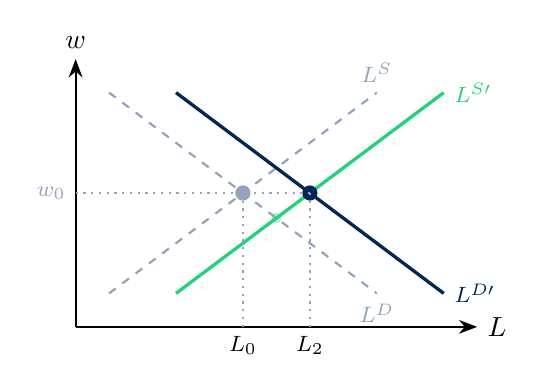
\begin{tikzpicture}[scale=0.85]
            % Axes
            \draw[-{Stealth}, thick] (0,0) -- (6,0) node[right] {$L$};
            \draw[-{Stealth}, thick] (0,0) -- (0,4) node[above] {$w$};
            % Original supply (dashed gray)
            \draw[HECgray, dashed, thick] (0.5,0.5) -- (4.5,3.5)
               node[above, font=\footnotesize] {$L^S$};
            % Original demand (dashed gray)
            \draw[HECgray, dashed, thick] (0.5,3.5) -- (4.5,0.5)
               node[below, font=\footnotesize] {$L^D$};
            % Shifted supply (green): y = 0.75x - 0.625
            \draw[HECgreen, very thick] (1.5,0.5) -- (5.5,3.5)
               node[right, font=\footnotesize] {$L^{S\prime}$};
            % Shifted demand (navy): y = -0.75x + 4.625
            \draw[HECnavy, very thick] (1.5,3.5) -- (5.5,0.5)
               node[right, font=\footnotesize] {$L^{D\prime}$};
            % E0: (2.5, 2.0)
            \filldraw[HECgray] (2.5,2.0) circle (3pt);
            % E1 faded: (3.0, 1.625)
            \filldraw[HECgreen, opacity=0.3] (3.0,1.625) circle (2pt);
            % E2: (3.5, 2.0)
            \filldraw[HECnavy] (3.5,2.0) circle (3pt);
            % Dotted lines
            \draw[dotted, thick, HECgray] (0,2.0) node[left, font=\footnotesize] {$w_0$} -- (3.5,2.0);
            \draw[dotted, thick, HECgray] (2.5,0) -- (2.5,2.0);
            \draw[dotted, thick, HECgray] (3.5,0) -- (3.5,2.0);
            \node[font=\footnotesize, below] at (2.5,0) {$L_0$};
            \node[font=\footnotesize, below] at (3.5,0) {$L_2$};
         \end{tikzpicture}
      \end{column}
   \end{columns}
\end{frame}

% --- Application 4 : L'inflation en récession --------------------------------

\begin{frame}{Récessions et chômage au Canada}
   \begin{figure}
      \centering
      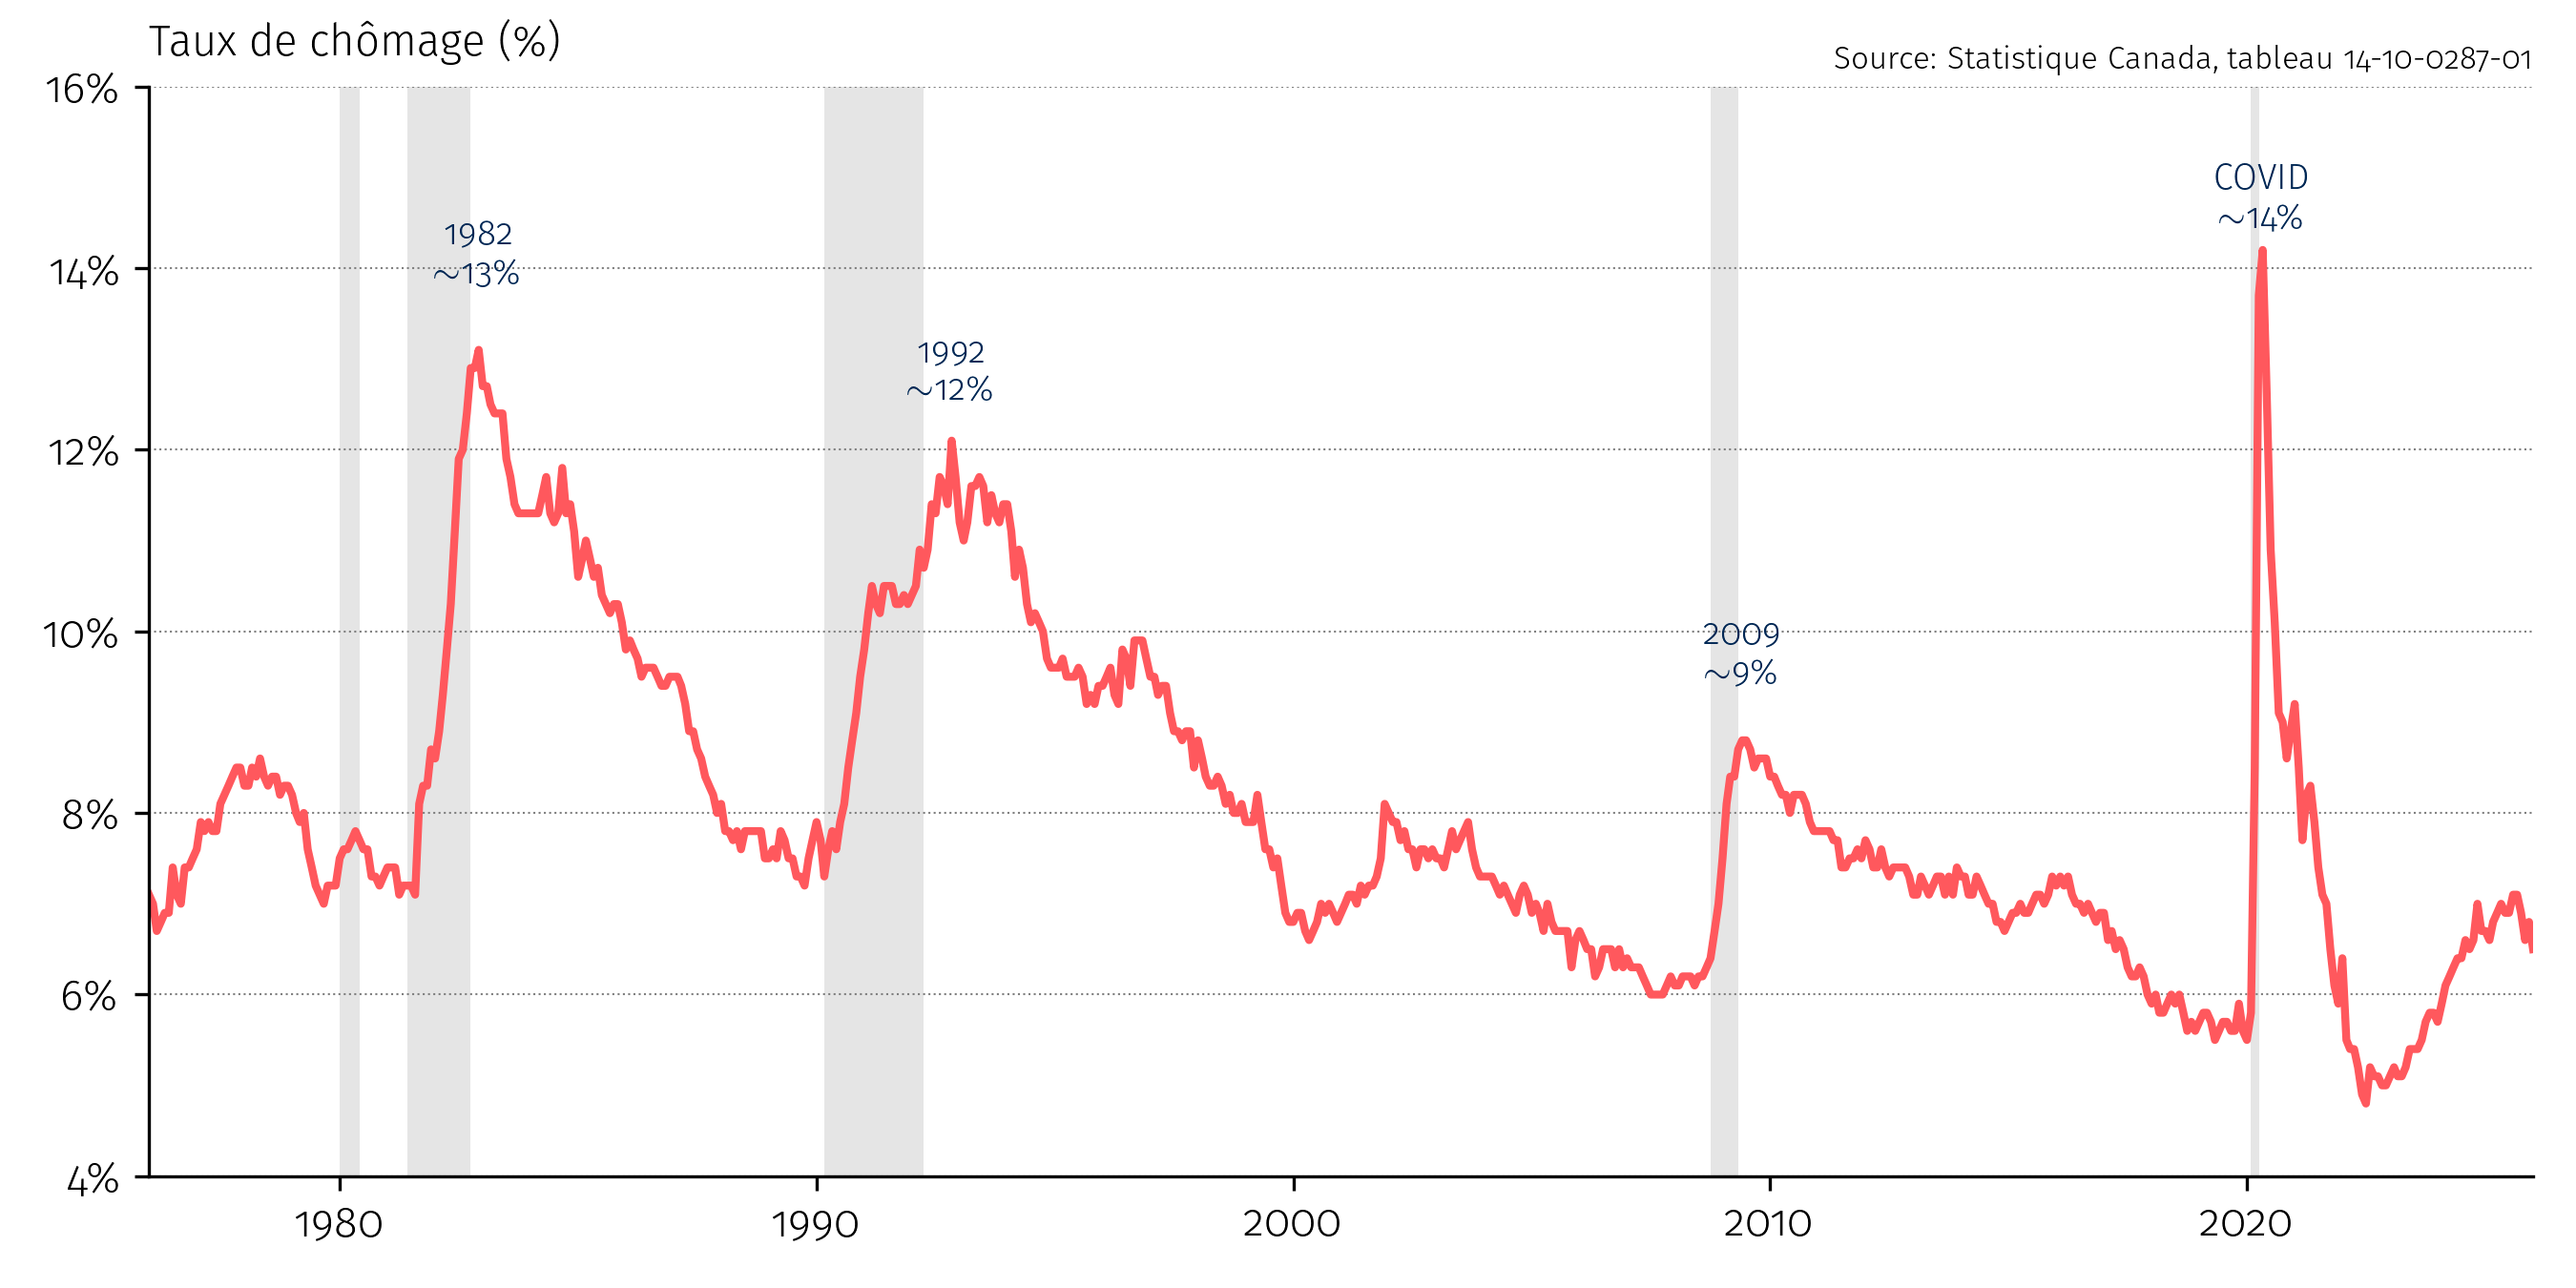
\includegraphics[width=0.95\textwidth]{unemployment_ca.png}
   \end{figure}
\end{frame}

\begin{frame}{Pourquoi les salaires ne baissent-ils pas?}
   \vspace{-0.5cm}
   \begin{defbox}[Rigidité nominale des salaires]
      Les salaires nominaux résistent fortement à la baisse, même en récession.
   \end{defbox}
   \vspace{0.3cm}
   Trois raisons principales :
   \vspace{0.15cm}
   \begin{itemize}
      \setlength\itemsep{0.2cm}
      \item \textbf{Conventions collectives} --- les salaires sont fixés par contrat pour 2--3 ans
      \item \textbf{Contrats implicites} --- baisser les salaires détruit le moral et la productivité
      \item \textbf{Normes sociales} --- une baisse de salaire est perçue comme une injustice
   \end{itemize}
   \vspace{0.3cm}
   Résultat : les entreprises préfèrent \textbf{licencier} que baisser les salaires.
\end{frame}

\begin{frame}{Pourquoi l'inflation aide en récession}
   Si les salaires nominaux ne peuvent pas baisser, comment rétablir l'équilibre?
   \vspace{0.3cm}

   \textbf{L'inflation} offre une solution élégante :
   \vspace{0.2cm}
   \begin{center}
      $\displaystyle w_{\text{réel}} = \frac{w_{\text{nominal}}}{P}$
   \end{center}
   \vspace{0.2cm}
   Si $P \uparrow$ et $w_{\text{nominal}}$ reste fixe $\to$ $w_{\text{réel}} \downarrow$ $\to$ retour vers l'équilibre.
   \vspace{0.3cm}

   Les travailleurs acceptent plus facilement une \textbf{stagnation} salariale avec 2\% d'inflation (baisse réelle invisible) qu'une \textbf{baisse nominale} de 2\%.
\end{frame}

\begin{frame}{Rigidité salariale : le modèle}
   \begin{columns}[c]
      \begin{column}{0.52\textwidth}
         \centering
         {\small\textbf{\textcolor{HECcoral}{Récession} --- $w$ rigide}}
         \par\vspace{1pt}
         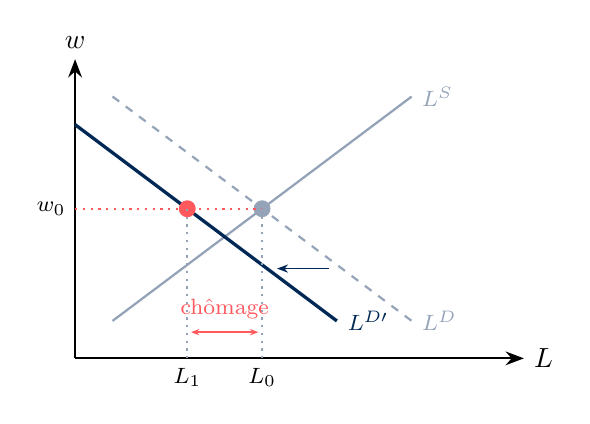
\begin{tikzpicture}[scale=0.95]
            % Axes
            \draw[-{Stealth}, thick] (0,0) -- (6,0) node[right] {$L$};
            \draw[-{Stealth}, thick] (0,0) -- (0,4) node[above] {$w$};
            % Supply (solid): y = 0.75x + 0.125
            \draw[HECgray, thick] (0.5,0.5) -- (4.5,3.5)
               node[right, font=\footnotesize] {$L^S$};
            % Original demand (dashed gray): y = -0.75x + 3.875
            \draw[HECgray, dashed, thick] (0.5,3.5) -- (4.5,0.5)
               node[right, font=\footnotesize] {$L^D$};
            % Shifted demand (navy, -1.0 left): y = -0.75x + 3.125
            \draw[HECnavy, very thick] (0,3.125) -- (3.5,0.5)
               node[right, font=\footnotesize] {$L^{D\prime}$};
            % E0: (2.5, 2.0)
            \filldraw[HECgray] (2.5,2.0) circle (3pt);
            % Rigid wage line at w0 = 2.0, from y-axis to L^S at w0 (x=2.5)
            \draw[HECcoral, thick, dotted] (0,2.0) -- (2.5,2.0);
            % At w0 on L^D': -0.75x + 3.125 = 2.0 → x = 1.5
            \filldraw[HECcoral] (1.5,2.0) circle (3pt);
            % Dotted lines to x-axis
            \draw[dotted, thick, HECgray] (2.5,0) -- (2.5,2.0);
            \draw[dotted, thick, HECgray] (1.5,0) -- (1.5,2.0);
            \node[font=\footnotesize, below] at (2.5,0) {$L_0$};
            \node[font=\footnotesize, below] at (1.5,0) {$L_1$};
            % Wage label on y-axis
            \node[font=\footnotesize, left] at (0,2.0) {$w_0$};
            % Unemployment bracket
            \draw[HECcoral, thick, {Stealth[length=3pt]}-{Stealth[length=3pt]}]
               (1.55,0.35) -- (2.45,0.35)
               node[midway, above=1pt, font=\footnotesize, HECcoral]
               {ch\^{o}mage};
            % Shift arrow (between L^D and L^D' at y=1.2)
            \draw[-{Stealth[length=4pt]}, HECnavy] (3.4,1.2) -- (2.7,1.2);
         \end{tikzpicture}
      \end{column}
      \begin{column}{0.52\textwidth}
         \centering
         {\small\textbf{\textcolor{HECnavy}{Avec inflation} --- $w_{\text{réel}} \downarrow$}}
         \par\vspace{1pt}
         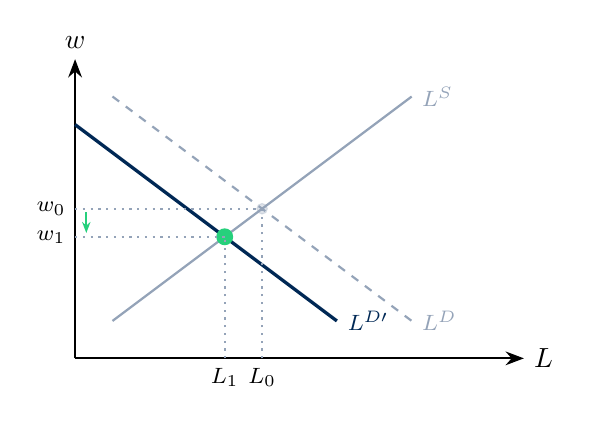
\begin{tikzpicture}[scale=0.95]
            % Axes
            \draw[-{Stealth}, thick] (0,0) -- (6,0) node[right] {$L$};
            \draw[-{Stealth}, thick] (0,0) -- (0,4) node[above] {$w$};
            % Supply (solid): y = 0.75x + 0.125
            \draw[HECgray, thick] (0.5,0.5) -- (4.5,3.5)
               node[right, font=\footnotesize] {$L^S$};
            % Original demand (dashed gray): y = -0.75x + 3.875
            \draw[HECgray, dashed, thick] (0.5,3.5) -- (4.5,0.5)
               node[right, font=\footnotesize] {$L^D$};
            % Shifted demand (navy): y = -0.75x + 3.125
            \draw[HECnavy, very thick] (0,3.125) -- (3.5,0.5)
               node[right, font=\footnotesize] {$L^{D\prime}$};
            % E0 faded: (2.5, 2.0)
            \filldraw[HECgray, opacity=0.3] (2.5,2.0) circle (2pt);
            % New equilibrium: L^S = L^D' → (2.0, 1.625)
            \filldraw[HECgreen] (2.0,1.625) circle (3pt);
            % Dotted lines to x-axis
            \draw[dotted, thick, HECgray] (2.5,0) -- (2.5,2.0);
            \draw[dotted, thick, HECgray] (2.0,0) -- (2.0,1.625);
            \node[font=\footnotesize, below] at (2.5,0) {$L_0$};
            \node[font=\footnotesize, below] at (2.0,0) {$L_1$};
            % Dotted lines to y-axis
            \draw[dotted, thick, HECgray] (0,2.0) -- (2.5,2.0);
            \draw[dotted, thick, HECgray] (0,1.625) -- (2.0,1.625);
            \node[font=\footnotesize, left] at (0,2.0) {$w_0$};
            \node[font=\footnotesize, left] at (0,1.625) {$w_1$};
            % Arrow on y-axis: inflation lowers real wage
            \draw[-{Stealth[length=4pt]}, HECgreen, thick]
               (0.15,1.95) -- (0.15,1.675);
         \end{tikzpicture}
      \end{column}
   \end{columns}
\end{frame}

% ============================================================================
\begin{frame}{Plan}
   \begin{enumerate}
      \setlength\itemsep{0.5cm}
      \item {\color{gray!50}Théories de la productivité}
      \item {\color{gray!50}Indicateurs du marché du travail}
      \item {\color{gray!50}Un modèle simple du marché du travail}
      \item {\color{gray!50}Applications du modèle}
      \item \textbf{Technologie, IA, et inégalités}
   \end{enumerate}
\end{frame}

% ============================================================================
\sectionframe{Technologie, IA, et inégalités}
% ============================================================================

\begin{frame}{Les inégalités augmentent dans les pays riches}
   \begin{figure}
      \centering
      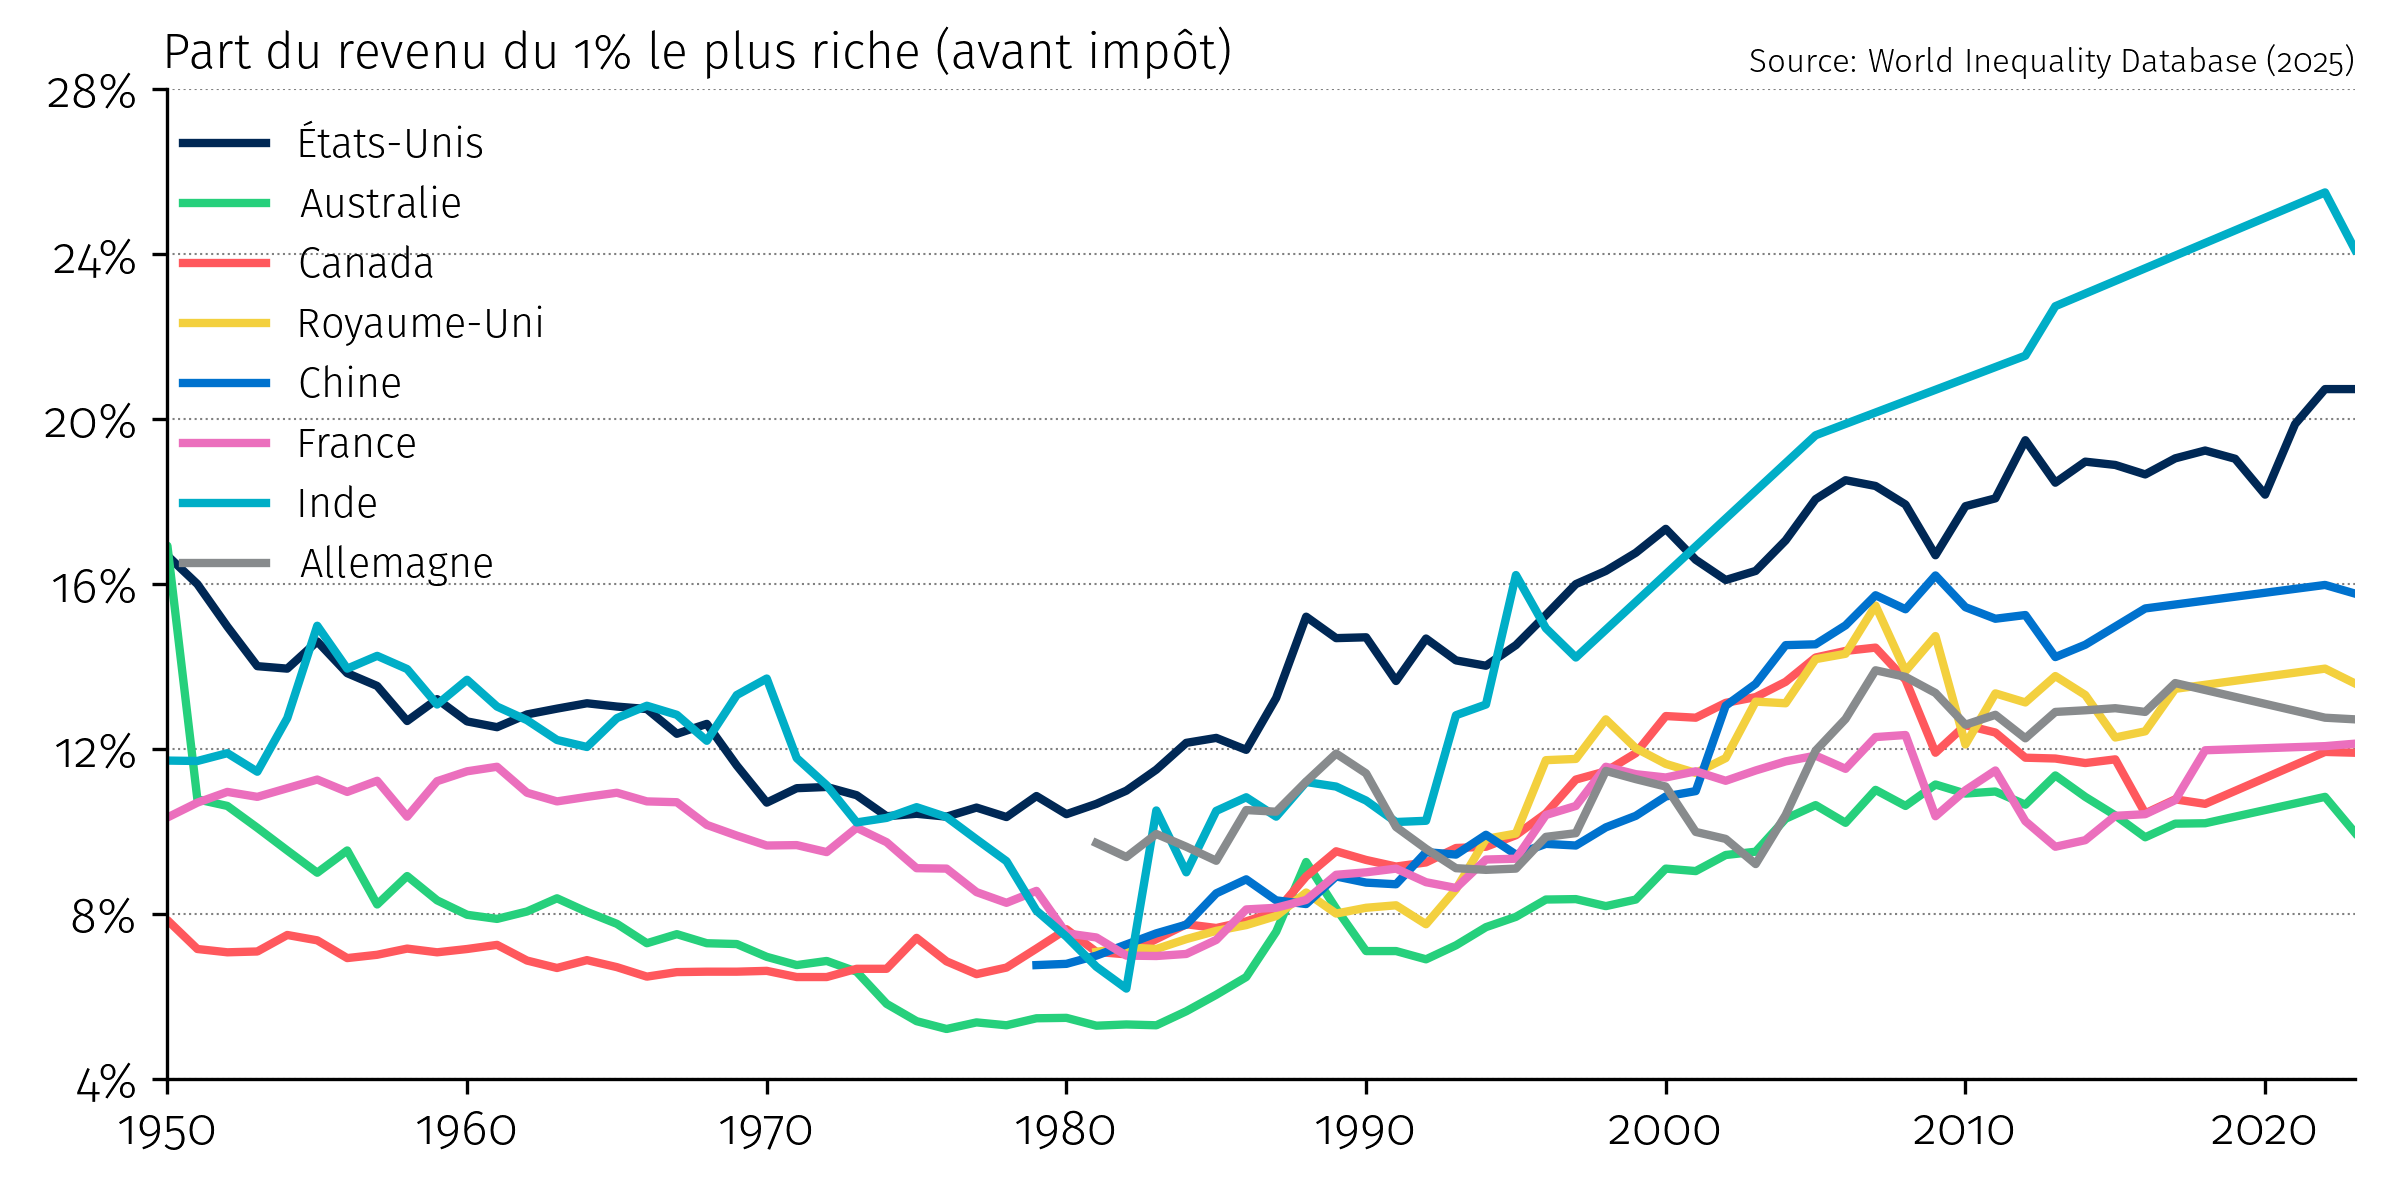
\includegraphics[width=0.9\textwidth, height=0.75\textheight, keepaspectratio]{inequality_within_countries.png}
   \end{figure}
\end{frame}

\begin{frame}{La courbe de l'éléphant}
   \vspace{-0.2cm}
   \begin{figure}
      \centering
      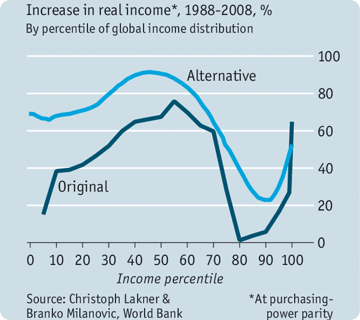
\includegraphics[width=0.85\textwidth, height=0.55\textheight, keepaspectratio]{elephant.png}
   \end{figure}
   \vspace{-0.2cm}
   \begin{keyinsight}
      \small Les grands gagnants de la mondialisation : les classes moyennes des pays émergents et les très riches. Les grands perdants : les classes moyennes et ouvrières des pays avancés.
   \end{keyinsight}
\end{frame}

\begin{frame}[t]{Explication 1 : le progrès technique biaisé}
   \small
   \begin{columns}[T]
      \begin{column}{0.53\textwidth}
         Le changement technologique depuis les années 1980 favorise les travailleurs \textbf{qualifiés} :
         \vspace{0.1cm}
         \begin{itemize}
            \setlength\itemsep{0.1cm}
            \item Les TIC augmentent la demande de compétences cognitives non routinières
            \item Les tâches \textbf{routinières} (manufacturières, administratives) sont automatisées
            \item $L^D_{\text{qualifiés}} \uparrow$ et $L^D_{\text{non-qualifiés}} \downarrow$
         \end{itemize}
         \vspace{0.1cm}
         $\to$ Écart salarial croissant entre qualifiés et non-qualifiés
      \end{column}
      \begin{column}{0.44\textwidth}
         \centering
         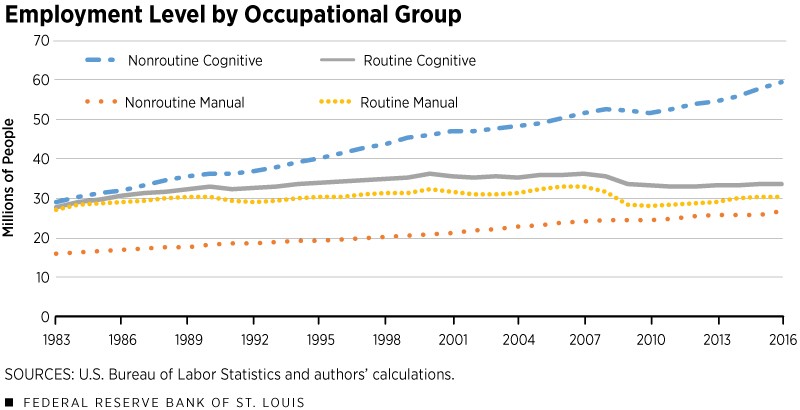
\includegraphics[width=\textwidth, keepaspectratio]{routine_vs_nonroutine_jobs.jpg}\\[4pt]
         {\footnotesize\textcolor{HECgray}{Emplois routiniers vs non routiniers}}
      \end{column}
   \end{columns}
\end{frame}

\begin{frame}{Le \textit{skill premium}}
   \begin{figure}
      \centering
      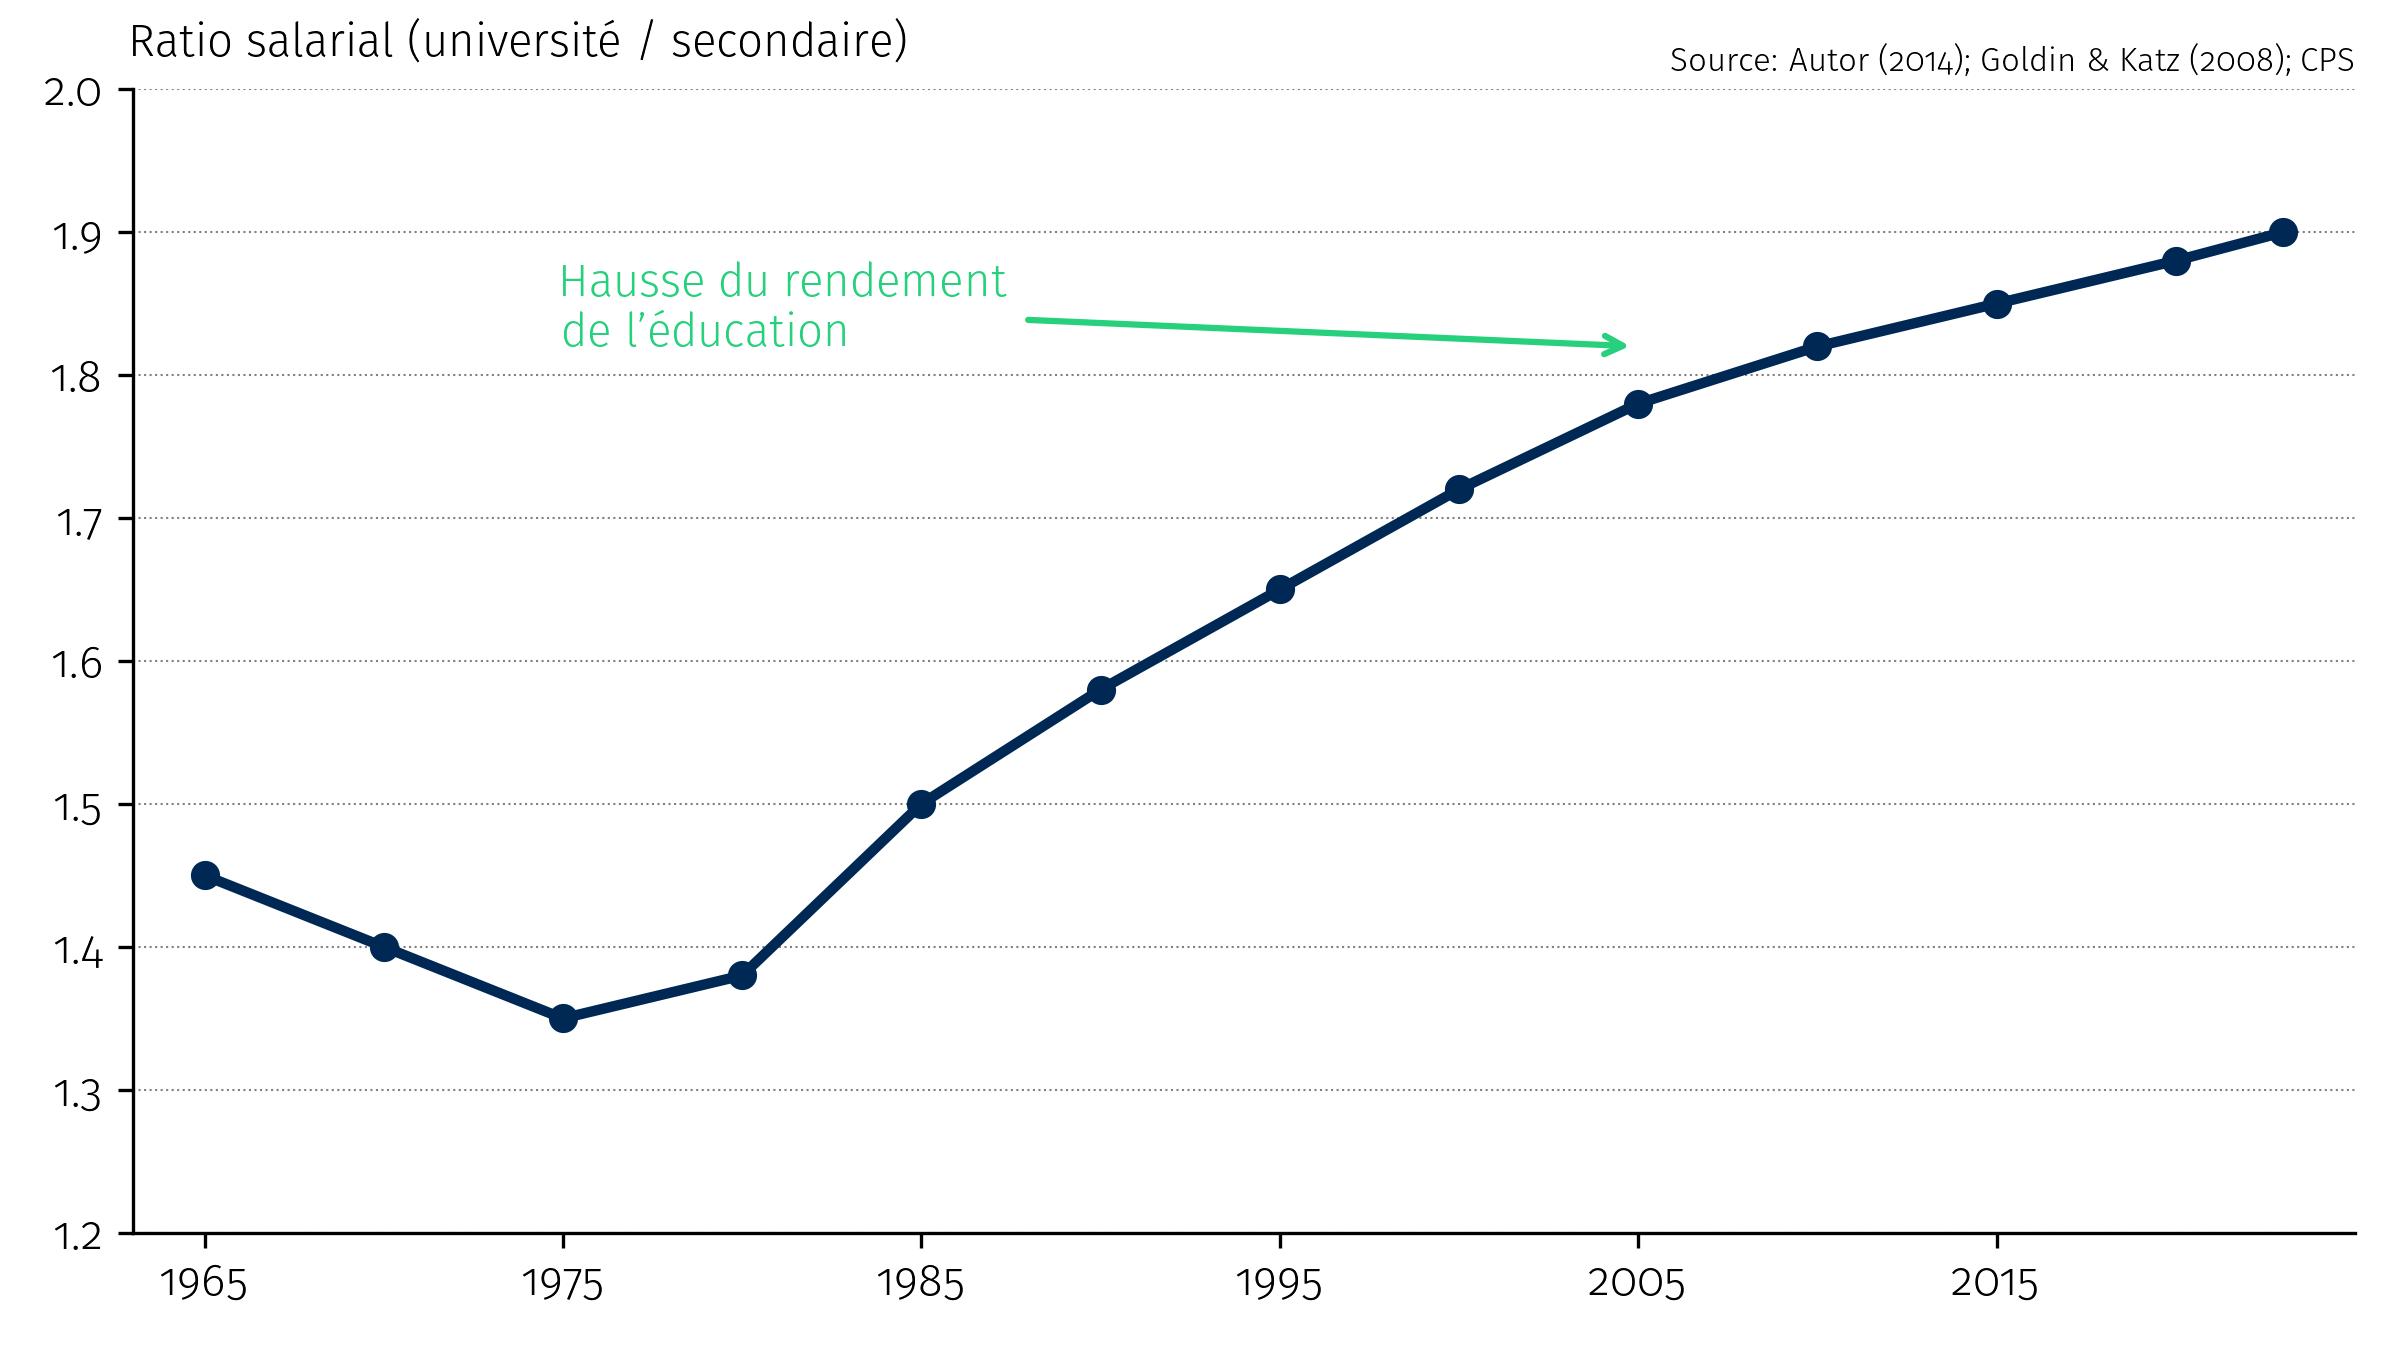
\includegraphics[width=0.9\textwidth, height=0.75\textheight, keepaspectratio]{inequality_skill_premium.png}
   \end{figure}
\end{frame}

\begin{frame}[t]{Explication 2 : la mondialisation et le choc chinois}
   \small
   \begin{columns}[T]
      \begin{column}{0.53\textwidth}
         \textbf{Autor, Dorn \& Hanson (2013)} : l'entrée de la Chine à l'OMC (2001) a provoqué un choc massif sur les marchés du travail américains.
         \vspace{0.1cm}
         \begin{itemize}
            \setlength\itemsep{0.1cm}
            \item Régions exposées aux importations chinoises : chômage $\uparrow$, salaires $\downarrow$, transferts sociaux $\uparrow$
            \item Effets \textbf{persistants} sur 15+ ans
            \item Les travailleurs déplacés ne se reconvertissent pas facilement
         \end{itemize}
      \end{column}
      \begin{column}{0.44\textwidth}
         \centering
         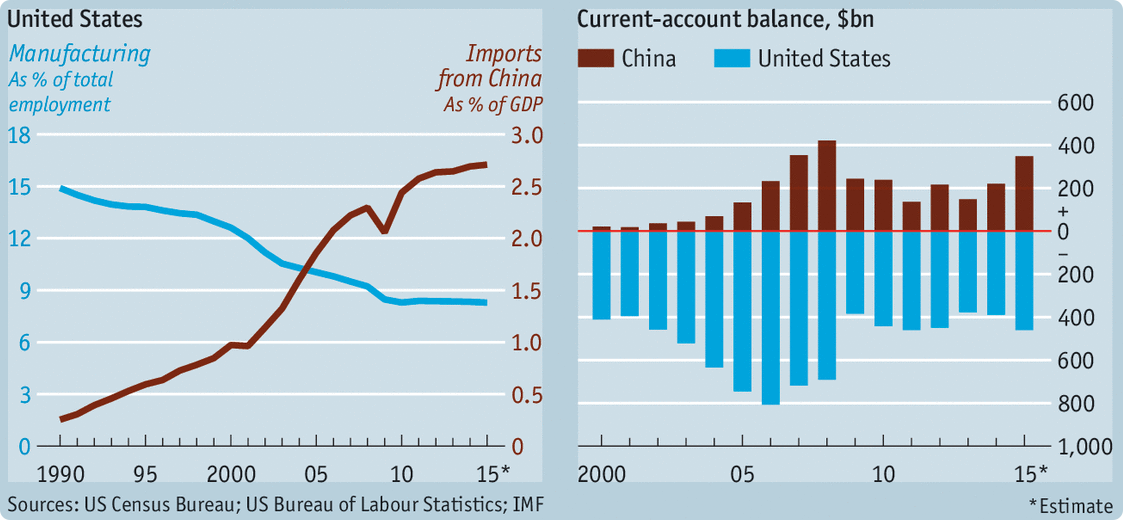
\includegraphics[width=\textwidth, keepaspectratio]{china_shock.png}\\[4pt]
         {\footnotesize\textcolor{HECgray}{Le \guillemotleft~choc chinois~\guillemotright\ sur l'emploi manufacturier}}
      \end{column}
   \end{columns}
\end{frame}

\begin{frame}[t]{Explication 3 : l'érosion des institutions}
   \begin{warning}[Facteurs institutionnels]
      \begin{itemize}
         \setlength\itemsep{0.15cm}
         \item \textbf{Déclin de la syndicalisation :} de $\sim$35\,\% dans les années 1950 à $\sim$10\,\% aujourd'hui (États-Unis). Moins de pouvoir de négociation pour les bas salaires.
         \item \textbf{Salaire minimum stagnant :} en termes réels, le salaire minimum fédéral américain est plus bas qu'en 1968.
         \item \textbf{Fiscalité régressive :} taux marginaux supérieurs en baisse depuis les années 1980 (de 70\,\% à 37\,\% aux États-Unis).
         \item \textbf{Concentration du marché :} moins de concurrence $\to$ rentes captées par les entreprises dominantes.
      \end{itemize}
   \end{warning}
\end{frame}

\begin{frame}[t]{La courbe de Gatsby}
   \vspace{-0.2cm}
   \begin{figure}
      \centering
      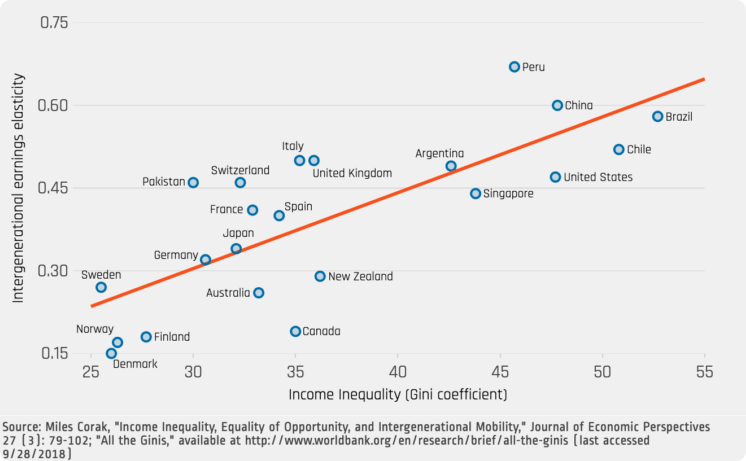
\includegraphics[width=0.8\textwidth, height=0.5\textheight, keepaspectratio]{gatsby.png}
   \end{figure}
   \vspace{-0.2cm}
   \begin{keyinsight}
      \small Plus les inégalités de \textbf{revenus} sont élevées dans un pays, plus la \textbf{mobilité intergénérationnelle} est faible. L'inégalité des résultats et l'inégalité des chances sont \textbf{liées}.
   \end{keyinsight}
\end{frame}

\begin{frame}[t]{La part du travail dans le PIB diminue}
   \vspace{-0.2cm}
   \begin{figure}
      \centering
      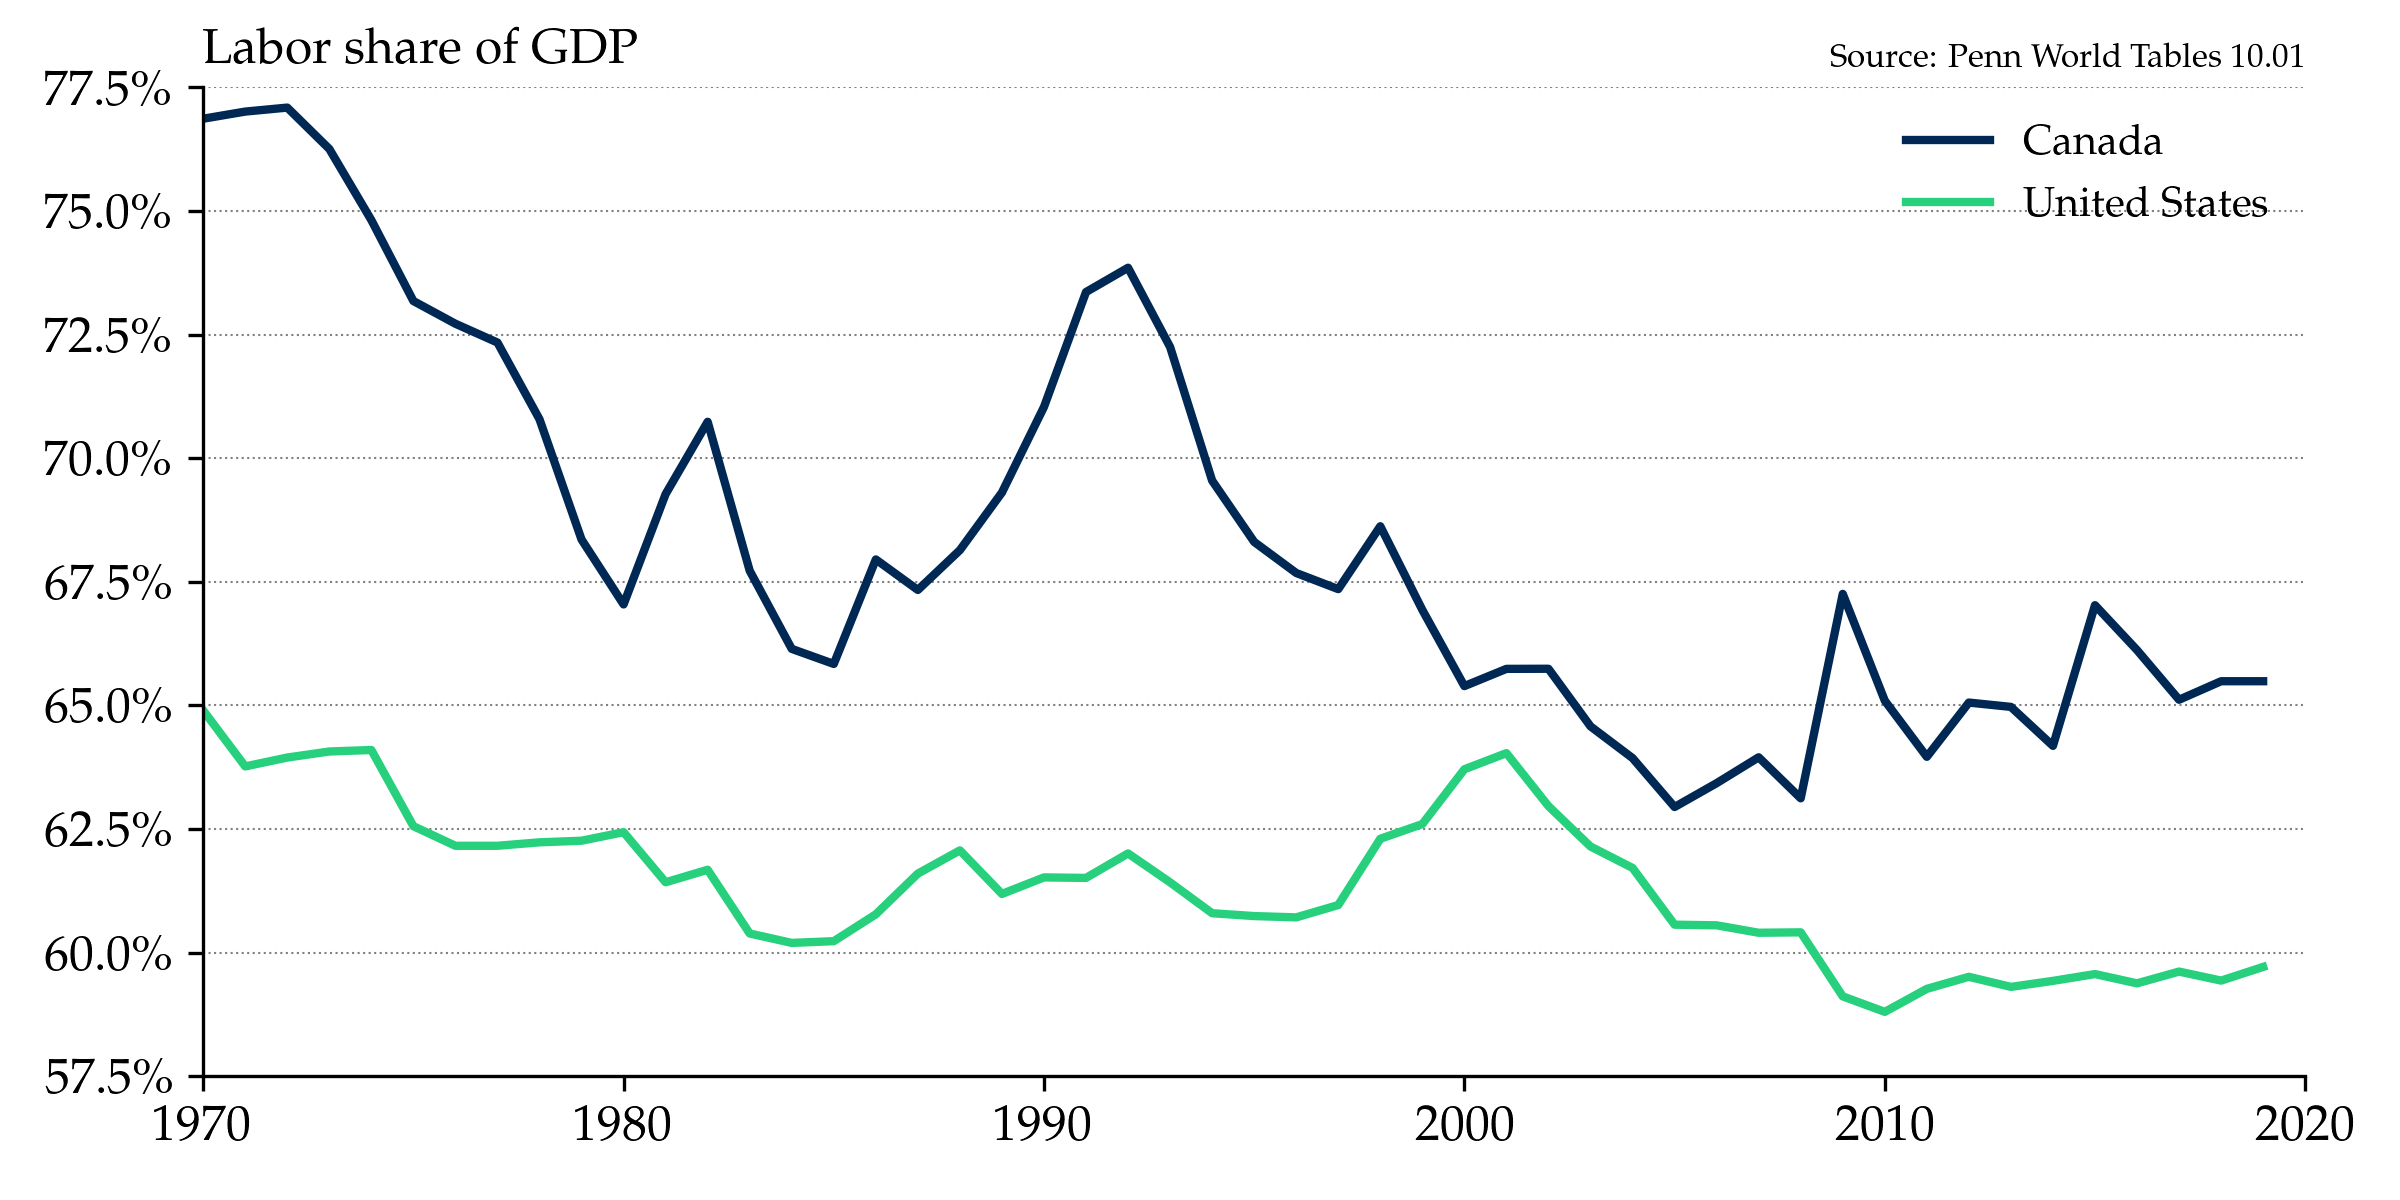
\includegraphics[width=0.85\textwidth, height=0.5\textheight, keepaspectratio]{labor_share_canada_usa.png}
   \end{figure}
   \vspace{-0.3cm}
   \small
   La part du revenu national versée au travail a diminué de $\sim$5 points de pourcentage depuis 1980. Cette baisse est concentrée dans le secteur manufacturier et reflète la réallocation vers des entreprises à faible part du travail (Kehrig \& Vincent, 2021).
\end{frame}

% ============================================================================
\begin{frame}{Plan}
   \begin{enumerate}
      \setlength\itemsep{0.25cm}
      \item {\color{gray!50}Théories de la productivité}
      \item {\color{gray!50}Indicateurs du marché du travail}
      \item {\color{gray!50}Un modèle simple d'offre et de demande}
      \item {\color{gray!50}Applications}
      \item {\color{gray!50}Inégalités et mondialisation}
      \item \textbf{IA et l'avenir du travail}
   \end{enumerate}
\end{frame}

% ============================================================================
\sectionframe{IA et l'avenir du travail}
% ============================================================================

\begin{frame}[t]{L'IA va-t-elle tout changer?}
   \small
   L'IA est la dernière vague d'une longue histoire d'automatisation :
   \vspace{0.2cm}
   \begin{itemize}
      \setlength\itemsep{0.15cm}
      \item \textbf{Métiers à tisser} (XIXe s.) : les Luddites craignaient la fin du travail
      \item \textbf{Guichets automatiques} (1970s) : n'ont \textit{pas} éliminé les caissiers de banque --- ils ont transformé leur rôle (vers le conseil et la vente)
      \item \textbf{Robots industriels} (1990s) : ont remplacé des emplois manufacturiers mais créé des emplois en maintenance et programmation
   \end{itemize}
   \vspace{0.15cm}
   \begin{keyinsight}
      Historiquement, la technologie \textbf{transforme} les emplois plus qu'elle ne les \textbf{détruit}. Mais la vitesse et l'ampleur de l'IA pourraient être différentes.
   \end{keyinsight}
\end{frame}

\begin{frame}[t]{Tâches routinières vs non routinières}
   \small
   \begin{columns}[T]
      \begin{column}{0.48\textwidth}
         \textbf{\textcolor{HECcoral}{Automatisable :}}
         \vspace{0.1cm}
         \begin{itemize}
            \setlength\itemsep{0.1cm}
            \item Routinier \textbf{manuel} : assemblage, tri, conduite
            \item Routinier \textbf{cognitif} : comptabilité, saisie de données, traduction simple
         \end{itemize}
         \vspace{0.2cm}
         $\to$ L'IA touche désormais les tâches \textbf{cognitives}, pas seulement manuelles
      \end{column}
      \begin{column}{0.48\textwidth}
         \textbf{\textcolor{HECnavy}{Difficilement automatisable :}}
         \vspace{0.1cm}
         \begin{itemize}
            \setlength\itemsep{0.1cm}
            \item Non routinier \textbf{cognitif} : créativité, jugement, stratégie
            \item Non routinier \textbf{manuel} : soins, construction, réparation
         \end{itemize}
         \vspace{0.2cm}
         $\to$ Compétences de \textbf{résolution de problèmes} et d'\textbf{interaction humaine}
      \end{column}
   \end{columns}
   \vspace{0.2cm}
   \begin{warning}
      Les emplois \guillemotleft~du milieu~\guillemotright\ disparaissent : c'est la \textbf{polarisation} du marché du travail.
   \end{warning}
\end{frame}

\begin{frame}[t]{Les gagnants et les perdants}
   \footnotesize
   \textbf{Qui bénéficie de l'IA?}
   \vspace{0.05cm}
   \begin{itemize}
      \setlength\itemsep{0.05cm}
      \item Travailleurs hautement qualifiés qui \textbf{complémentent} l'IA (analystes, ingénieurs, chercheurs)
      \item Entreprises qui adoptent l'IA rapidement (avantage concurrentiel)
      \item Consommateurs (baisse de prix, nouveaux produits)
   \end{itemize}
   \vspace{0.1cm}

   \textbf{Qui est à risque?}
   \vspace{0.05cm}
   \begin{itemize}
      \setlength\itemsep{0.05cm}
      \item Travailleurs de compétences moyennes dans des tâches \textbf{routinières cognitives}
      \item Secteurs entiers : centres d'appels, comptabilité de base, traduction
      \item Régions dépendantes d'un seul secteur exposé
   \end{itemize}
   \vspace{0.1cm}
   \begin{keyinsight}
      L'IA ne remplace pas des \textbf{métiers} entiers --- elle remplace des \textbf{tâches}. Les travailleurs qui s'adaptent en seront les gagnants.
   \end{keyinsight}
\end{frame}

\begin{frame}[t]{Capital et travail à l'ère de l'IA}
   \small
   \textbf{Moll, Rachel \& Restrepo (2022)} posent la question centrale :
   \vspace{0.15cm}

   Si l'IA peut \textbf{substituer} le travail à grande échelle, les gains de productivité iront principalement au \textbf{capital} (les propriétaires des systèmes d'IA).
   \vspace{0.2cm}

   \begin{columns}[T]
      \begin{column}{0.48\textwidth}
         \textbf{Scénario optimiste :}
         \vspace{0.1cm}
         \begin{itemize}
            \setlength\itemsep{0.1cm}
            \item IA = outil qui \textbf{augmente} la productivité des travailleurs
            \item Nouveaux emplois créés
            \item Gains partagés
         \end{itemize}
      \end{column}
      \begin{column}{0.48\textwidth}
         \textbf{Scénario pessimiste :}
         \vspace{0.1cm}
         \begin{itemize}
            \setlength\itemsep{0.1cm}
            \item IA = \textbf{substitut} au travail humain
            \item Part du travail $\downarrow\downarrow$
            \item Inégalités capital/travail explosent
         \end{itemize}
      \end{column}
   \end{columns}
   \vspace{0.15cm}
   \begin{warning}
      Si l'IA se substitue au travail, la majorité des gains pourraient revenir aux \textbf{propriétaires du capital}. La question distributive est au cœur du débat.
   \end{warning}
\end{frame}

\begin{frame}[t]{Le rôle des politiques publiques}
   \small
   \begin{bizimplication}[Préparer la transition]
      \begin{itemize}
         \setlength\itemsep{0.1cm}
         \item \textbf{Éducation et formation :} compétences complémentaires à l'IA (créativité, jugement, résolution de problèmes)
         \item \textbf{Filets de sécurité :} assurance-emploi adaptée, formation continue financée
         \item \textbf{Politique de concurrence :} éviter les monopoles de l'IA
         \item \textbf{Fiscalité :} repenser la taxation du capital vs le travail
      \end{itemize}
   \end{bizimplication}
   \vspace{0.1cm}
   \begin{keyinsight}
      Les entreprises qui investissent dans la \textbf{requalification} de leurs employés auront un avantage concurrentiel dans la transition vers l'IA.
   \end{keyinsight}
\end{frame}

% ============================================================================

\begin{frame}[t]{Résumé}
   \footnotesize
   \begin{keyinsight}[Productivité, travail et inégalités]
      \begin{enumerate}
         \setlength\itemsep{0.1cm}
         \item La \textbf{productivité} est le seul moteur de la croissance de long terme --- le Canada souffre d'un déficit chronique
         \item Les \textbf{idées} (non rivales) et les \textbf{institutions} sont les déterminants profonds de la PTF
         \item Le marché du travail s'analyse par \textbf{offre et demande} --- le capital s'ajuste à long terme
         \item Les inégalités croissantes reflètent le progrès technique biaisé, la mondialisation et l'érosion des institutions
         \item L'IA va transformer le marché du travail --- les gagnants seront ceux qui \textbf{complémentent} la technologie
      \end{enumerate}
   \end{keyinsight}
\end{frame}

% ============================================================================
\sectionframe{Avant la prochaine séance}
% ============================================================================

\begin{frame}[t]{Avant la prochaine séance}
   \textbf{Lectures suggérées :}
   \vspace{0.15cm}
   \begin{itemize}
      \setlength\itemsep{0.15cm}
      \item Autor, \guillemotleft~Work of the Past, Work of the Future~\guillemotright\ (2019)
      \item \textit{The Economist}, \guillemotleft~AI and the future of work~\guillemotright
      \item OECD, \guillemotleft~Objectif croissance~\guillemotright, fiche Canada (2024)
   \end{itemize}
   \vspace{0.3cm}
   \textbf{Question de réflexion :}
   \vspace{0.15cm}

   \begin{tcolorbox}[
      colback=HECnavy!5, colframe=HECnavy, arc=8pt,
      leftrule=3pt, boxrule=0pt,
      left=10pt, right=10pt, top=6pt, bottom=6pt
   ]
      Le Canada peut-il utiliser l'IA pour combler son déficit de productivité? Quels secteurs canadiens seraient les plus transformés? Utilisez le cadre de la mauvaise allocation des ressources pour structurer votre réponse.
   \end{tcolorbox}
   \vspace{0.3cm}
   \textbf{Prochaine séance :} Monnaie, inflation et cycles économiques
\end{frame}

\end{document}
